% -*- mode: fundamental -*-

% Slides for 2-hour tutorial
%   at RISC-V Summit, Oct 22, 2025, Santa Clara
% Title: "Learn to Design and Verify a 6-stage pipelined RISC-V CPU"

% Copyright (c) 2025 Rishiyur S. Nikhil, All Rights Reserved

% -*- mode: fundamental -*-

% Copyright (c) 2025 Rishiyur S. Nikhil, All Rights Reserved

% Preamble that is shareable across slide decks

\documentclass[10pt, aspectratio=169]{beamer}

% \documentclass[17pt]{beamer}

% Avail. font sizes: 8pt, 9pt, 10pt, 11pt, 12pt, 14pt, 17pt, 20pt.
% Default font size is 11pt (= 22pt in full screen mode).

\usepackage{verbatim}
\usepackage{fancyvrb}

% ================================================================
% Themes

\usetheme{Madrid}          % Line at bottom: Author (affiliation), OptTitle, Conf, page 

% \usetheme{Copenhagen}    % Same as Madrid except bottom line: Author, OptTitle

% \usetheme{Berkeley}    % Takes up 1-inch border on left and top

% ----------------
% colorthemes
% (default), beaver, beetle, seahorse, wolverine

\usecolortheme{seahorse}

% ================================================================
% Customization: show table of contents before each section
% Use \AtBeginSubsection    to show before each subsection

% \AtBeginSection[]
% {
%   \begin{frame}
%     \frametitle{Table of Contents}
%     \tableofcontents[currentsection]
%   \end{frame}
% }

% ================================================================

% ----------------
% ITALICISE WORDS
\newcommand{\ie}{\emph{i.e.,}}
\newcommand{\eg}{\emph{e.g.,}}
\newcommand{\Eg}{\emph{E.g.,}}
\newcommand{\etc}{\emph{etc.}}
\newcommand{\via}{\emph{via}}
\newcommand{\vs}{\emph{vs.}}

% ----------------
% EMPTY BOXES OF VARIOUS WIDTHS, FOR INDENTATION
\newcommand{\hm}{\hspace*{1em}}
\newcommand{\hmm}{\hspace*{2em}}
\newcommand{\hmmm}{\hspace*{3em}}
\newcommand{\hmmmm}{\hspace*{4em}}

% ----------------
% Convenient widths

\newlength{\hlessmmm}
\setlength{\hlessmmm}{\textwidth}
\addtolength{\hlessmmm}{-3em}

\newlength{\hlessmmmm}
\setlength{\hlessmmmm}{\textwidth}
\addtolength{\hlessmmmm}{-4em}

% ----------------
% STRUTS
% HORIZONTAL STRUT.  One argument (width).
\newcommand{\hstrut}[1]{\hspace*{#1}}
% VERTICAL STRUT. Two arguments (offset from baseline, height).
\newcommand{\vstrut}[2]{\rule[#1]{0in}{#2}}
% ----------------
% ``TIGHTLIST'' ENVIRONMENT (no para space betwee items, small indent)
\newenvironment{tightlist}%
{\begin{list}{$\bullet$}{%
    \setlength{\topsep}{0in}
    \setlength{\partopsep}{0in}
    \setlength{\itemsep}{0in}
    \setlength{\parsep}{0in}
    \setlength{\leftmargin}{1.5em}
    \setlength{\rightmargin}{0in}
    \setlength{\itemindent}{0in}
}
}%
{\end{list}
}
% ----------------

% End of preamble
% ****************************************************************


\newcommand{\bsc}{\emph{bsc}}
\newcommand{\BSV}{\bf BSV}
\newcommand{\DRUM}{\bf Drum}
\newcommand{\FIFE}{\bf Fife}
\newcommand{\SAIL}{\bf Sail}
\newcommand{\RVFI}{\bf RVFI}
\newcommand{\TESTRIG}{\bf TestRIG}
\newcommand{\BLUESIM}{\bf BlueSim}
\newcommand{\VCD}{\bf VCD}
\newcommand{\BookRepo}{\url{https://github.com/rsnikhil/Learn_Bluespec_and_RISCV_Design}}

% Note: font sizes: \small > \footnotesize > \scriptsize > \tiny

% ****************************************************************
% Title page

\title[Design \& Verify 6-stage RISC-V CPU]
      {Learn to Design and Verify a 6-stage pipelined RISC-V CPU}

% \subtitle{foo\rule[0in]{0in}{4ex}}

\author[{\copyright} R.S.Nikhil]{Rishiyur S.~Nikhil, Cofounder and CTO, Bluespec, Inc.}

% \institute{Bluespec, Inc.}

\date{October 22, 2025}

% ****************************************************************

\begin{document}

% ================================================================

\begin{frame}[fragile]
 \titlepage

 \begin{center}
  {\small Tutorial at Developer's Day, RISC-V Summit, Santa Clara CA}

  
\includegraphics[height=1cm]{Figures/Bluespec_Logo_2022-10}

  \vspace*{2ex}

  {\scriptsize Slides version: 1.00}
 \end{center}
\end{frame}

% ****************************************************************
% ****************************************************************
% ****************************************************************

\section{Introduction}

% ================================================================

\begin{frame}[fragile]
\frametitle{The Plan for Today}

\begin{center}
 \begin{minipage}{0.55\textwidth}\scriptsize
  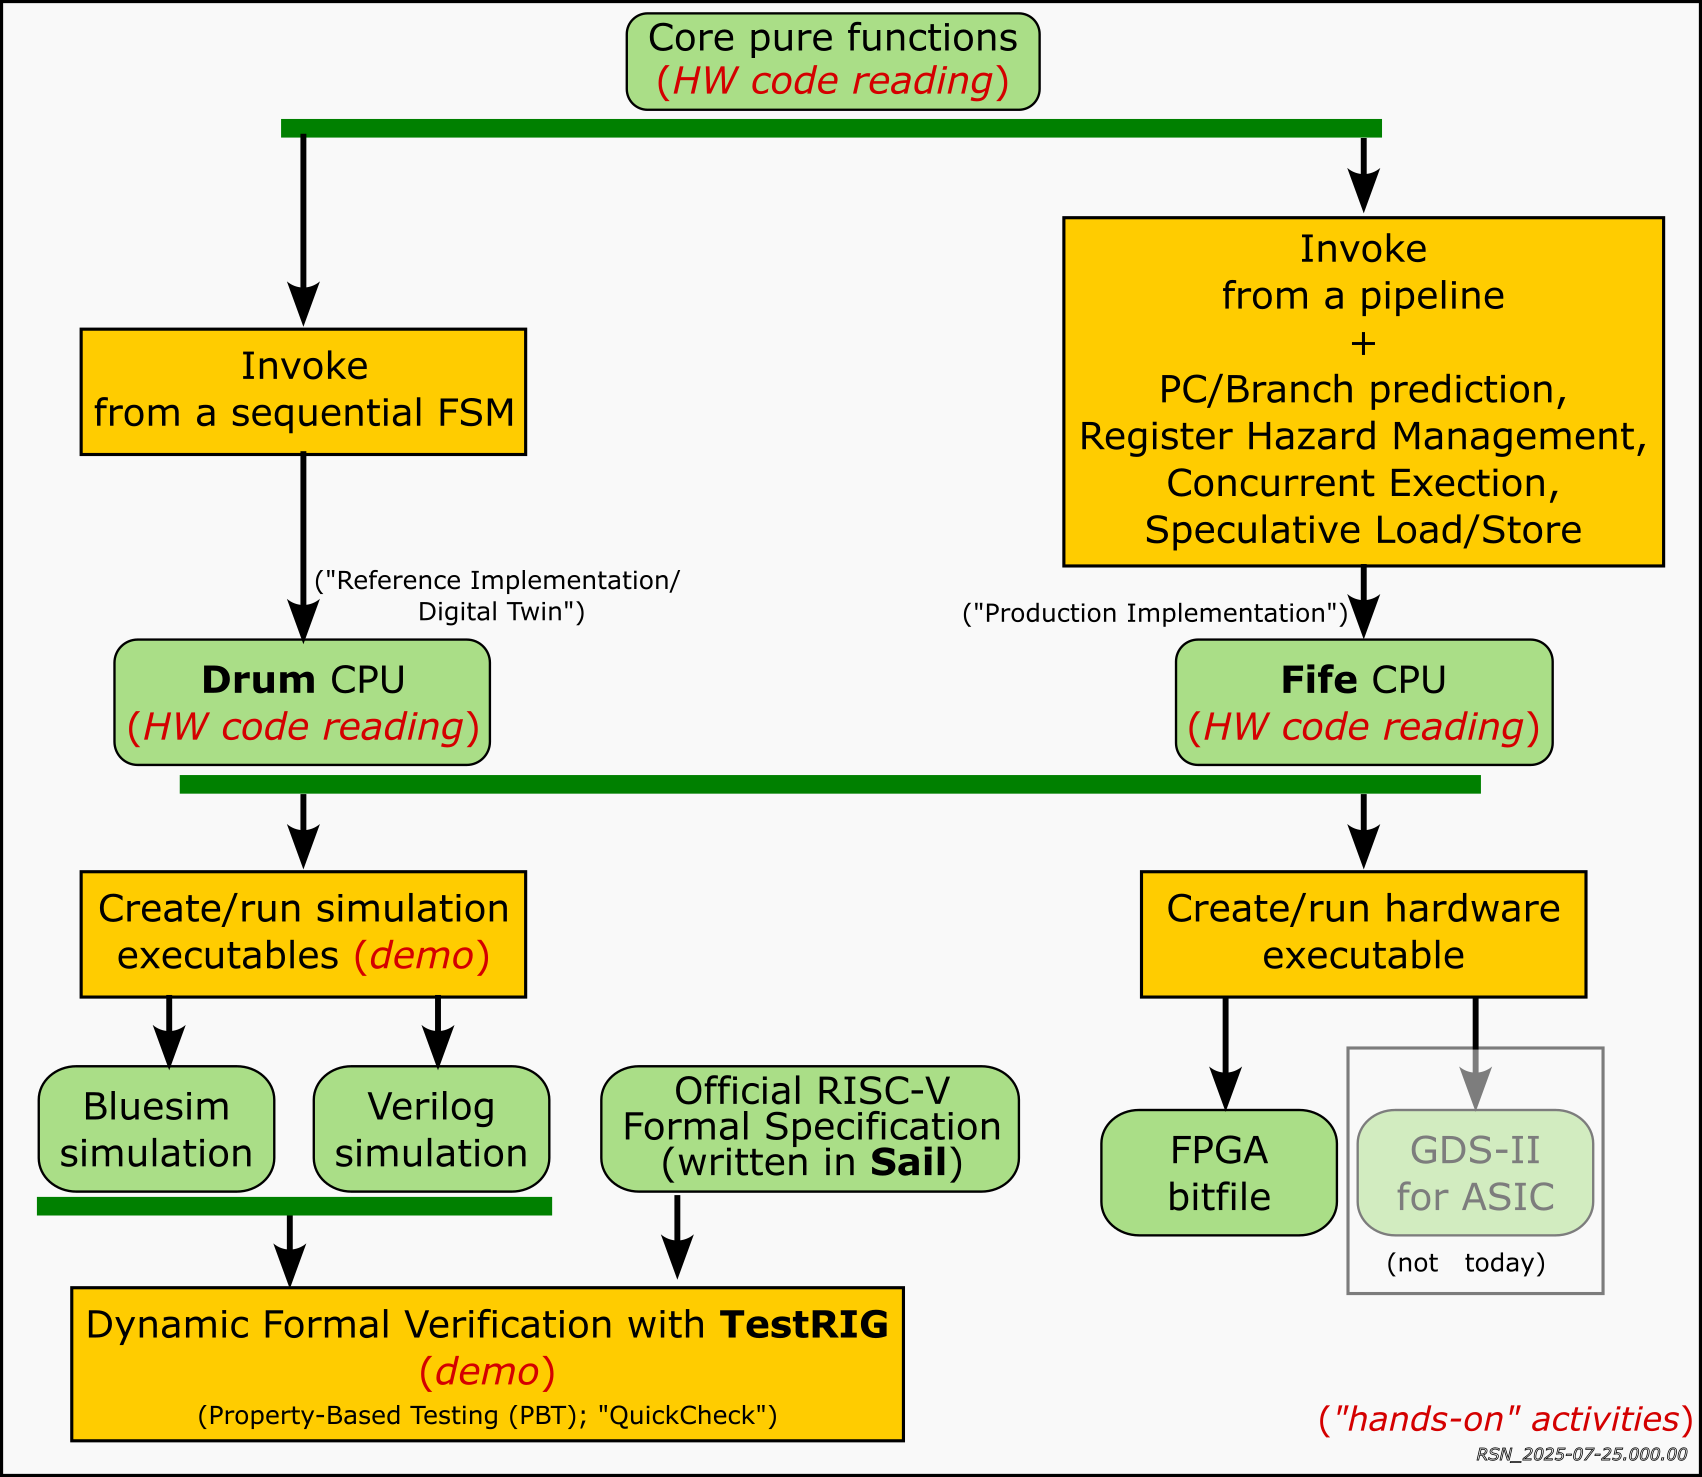
\includegraphics[width=\textwidth]{Figures/RSN_2025-07-25.000.00_Tutorial_Plan.png}
 \end{minipage}
 \begin{minipage}{0.44\textwidth}\scriptsize

  ``Hands on'':
  \begin{itemize}
   \item We will read the code together
   \item We create and run simulation executables together
   \item We will verify the design together
  \end{itemize}
  {\tiny (If you haven't installed the tools yet, please just listen
  and follow; hopefully you will try everything on your own, later)}

  \vspace{5ex}

  Not ``Hands on'' (lecture only):
  \begin{itemize}
   \item How to build and run on FPGA
  \end{itemize}

  \vspace{5ex}

  ``But I'm not familiar with hardware design'' or \\ ``I'm not familiar
  with the language used'' ...

  \hm ... don't worry:
  \begin{itemize}
   \item For "Core pure functions" and {\DRUM}, the code looks just like
         a conventional programming language

   \item {\FIFE} will introduce pipelining and pipeline techniques; we
         will explain the code in more detail.
  \end{itemize}
 \end{minipage}
\end{center}

\end{frame}

% ================================================================

\begin{frame}[fragile]

\frametitle{Prerequisites}

\begin{center}\scriptsize
 \begin{minipage}{0.9\textwidth}
  We \emph{do} assume that you are familiar with:
  \begin{itemize}

   \item Some ISA (Instruction Set Architecture): Machine Instructions
     and/or assembly-language (RISC-V or other).

     \vspace*{1ex}

     We're not going to explain what is a general-purpose register,
     what is a Program Counter, what is an arithmetic instruction,
     what is a BRANCH or JAL/JALR instruction, what is a LOAD/STORE
     instruction, etc.; we're assuming you already know these things.

   \vspace*{1ex}

   \item General coding (in C, Python, Go, Rust, Haskell, Verilog,
     SystemVerilog, ... whatever), so you can quickly grasp new,
     unfamiliar code.

     Familiarity with enum and struct types, functions, if-then-else.

     General knowledge of object-oriented programming is useful.
  \end{itemize}

  \vspace*{5ex}

  We \emph{do not} assume that you are familiar with:
  \begin{itemize}

   \item Hardware design, or any hardware design language (Verilog,
     SystemVerilog, Bluespec BSV or BH, Chisel, ...)

   \item Pipelined micro-architecture of CPUs

  \end{itemize}

  \vspace*{5ex}

  On the Tutorial Web Page
    (\url{https://github.com/rsnikhil/Tutorial_RISCV_Summit_2025}),
    we've asked you to install certain tools so that you can examine
    code and build and run things along with me during this tutorial.

  \vspace*{2ex}

  If you haven't done this already, then please just sit back and
  follow the lecture and demos, for now.  We hope that you will be
  motivated to later install the tools and try everything out for
  real.

 \end{minipage}
\end{center}

\end{frame}

% ================================================================

\begin{frame}[fragile]
\frametitle{Resources for this tutorial (all free and open-source)}

\begin{center}
 \begin{minipage}{\textwidth}\scriptsize
  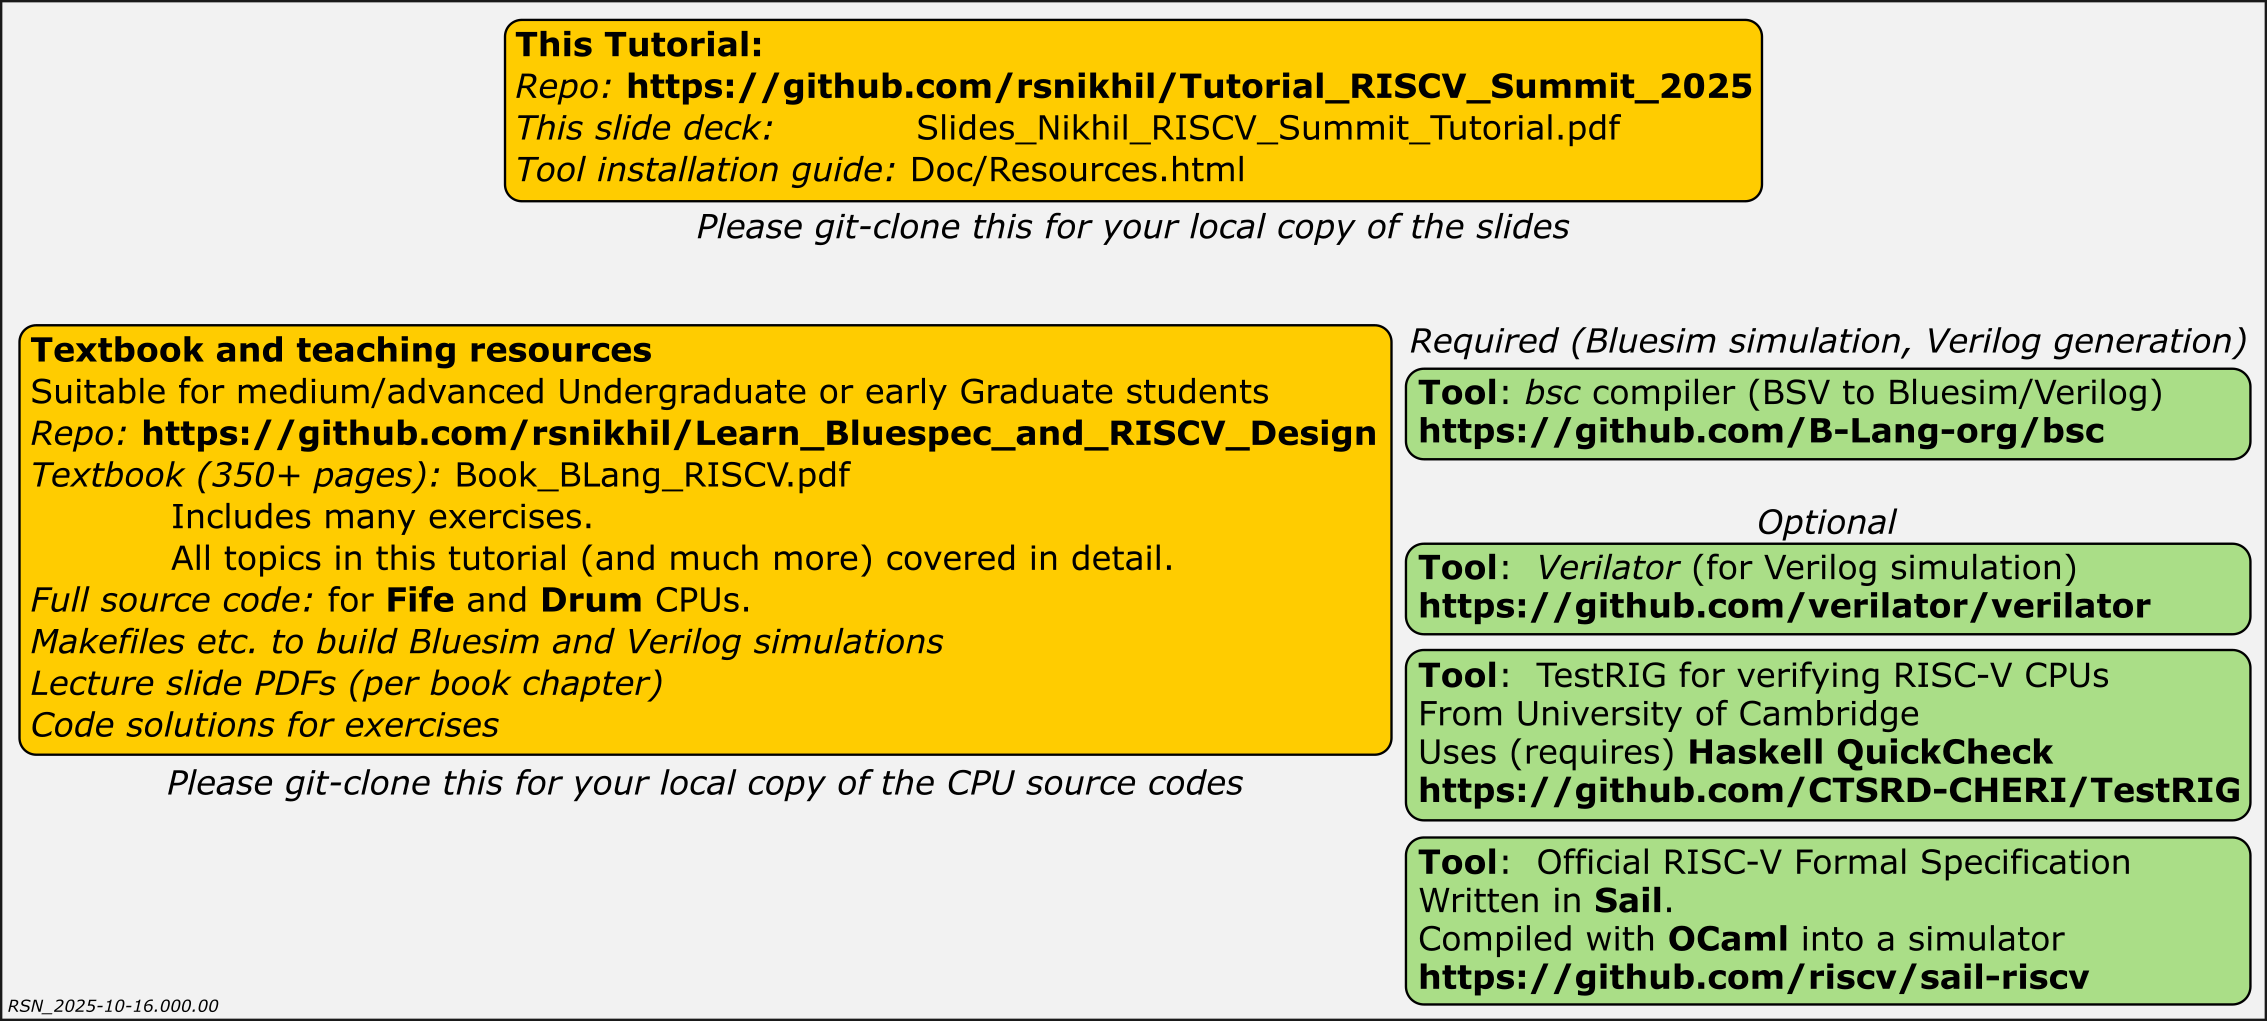
\includegraphics[width=\textwidth]
                  {Figures/RSN_2025-10-16.000.00_RISCV_Tutorial_Resources.png}
 \end{minipage}
\end{center}
\end{frame}

% ================================================================
% Verse interlude

\begin{frame}[fragile]

\begin{center}

 \fbox{
 \begin{minipage}{0.6\textwidth}\it
  \begin{tabbing}
    We have a {\bf lot} to get through, \\
    \hmm And just two hours to blow \\
    It'll be a bit of a fire hose \\
    \hmm Only a launchpad for more. \\
    \\
    So that's the plan; \\
    \hmm Don't panic, stay steady! \\
    It's really not so hard, \\
    \hmm Let's go! Are you ready!
  \end{tabbing}
 \end{minipage}}

 \vspace*{5ex}

 \begin{minipage}{0.6\textwidth}
  I'm sure you'll have more questions or follow-ups; \\
  please catch me at this Summit through tomorrow,  \\
  or email me later: \\
  \hm {\tt rsnikhil@pm.me} \\
  \hm {\tt nikhil@bluespec.com}
 \end{minipage}

\end{center}

\end{frame}

% ****************************************************************
% ****************************************************************
% ****************************************************************

\section{Core pure functions (shared by {\DRUM} and {\FIFE})}

\begin{frame}[fragile]

\frametitle{Contents}

\begin{center}
 \hmm
 \begin{minipage}{0.5\textwidth}
  \tableofcontents
 \end{minipage}
 \hmm
 \begin{minipage}{0.3\textwidth}
  \vstrut{0em}{20ex}
  \fbox{
   \begin{minipage}{\textwidth}\scriptsize\it
    {\bf Core pure functions}
    \begin{tabbing}
     Across many an implementation \\
     \hmm Certain functions are the same \\
     So, "Write once, Use many"; \\
     \hmm  This'll be our game.
    \end{tabbing}
   \end{minipage}}
 \end{minipage}
\end{center}

\end{frame}

% ================================================================

\begin{frame}[fragile]
\frametitle{Basic steps in executing an instruction (any CPU, incl. {\DRUM} and {\FIFE})}

\label{slide_instr_exec_steps}

\begin{center}
 \begin{minipage}{0.8\textwidth}\scriptsize
  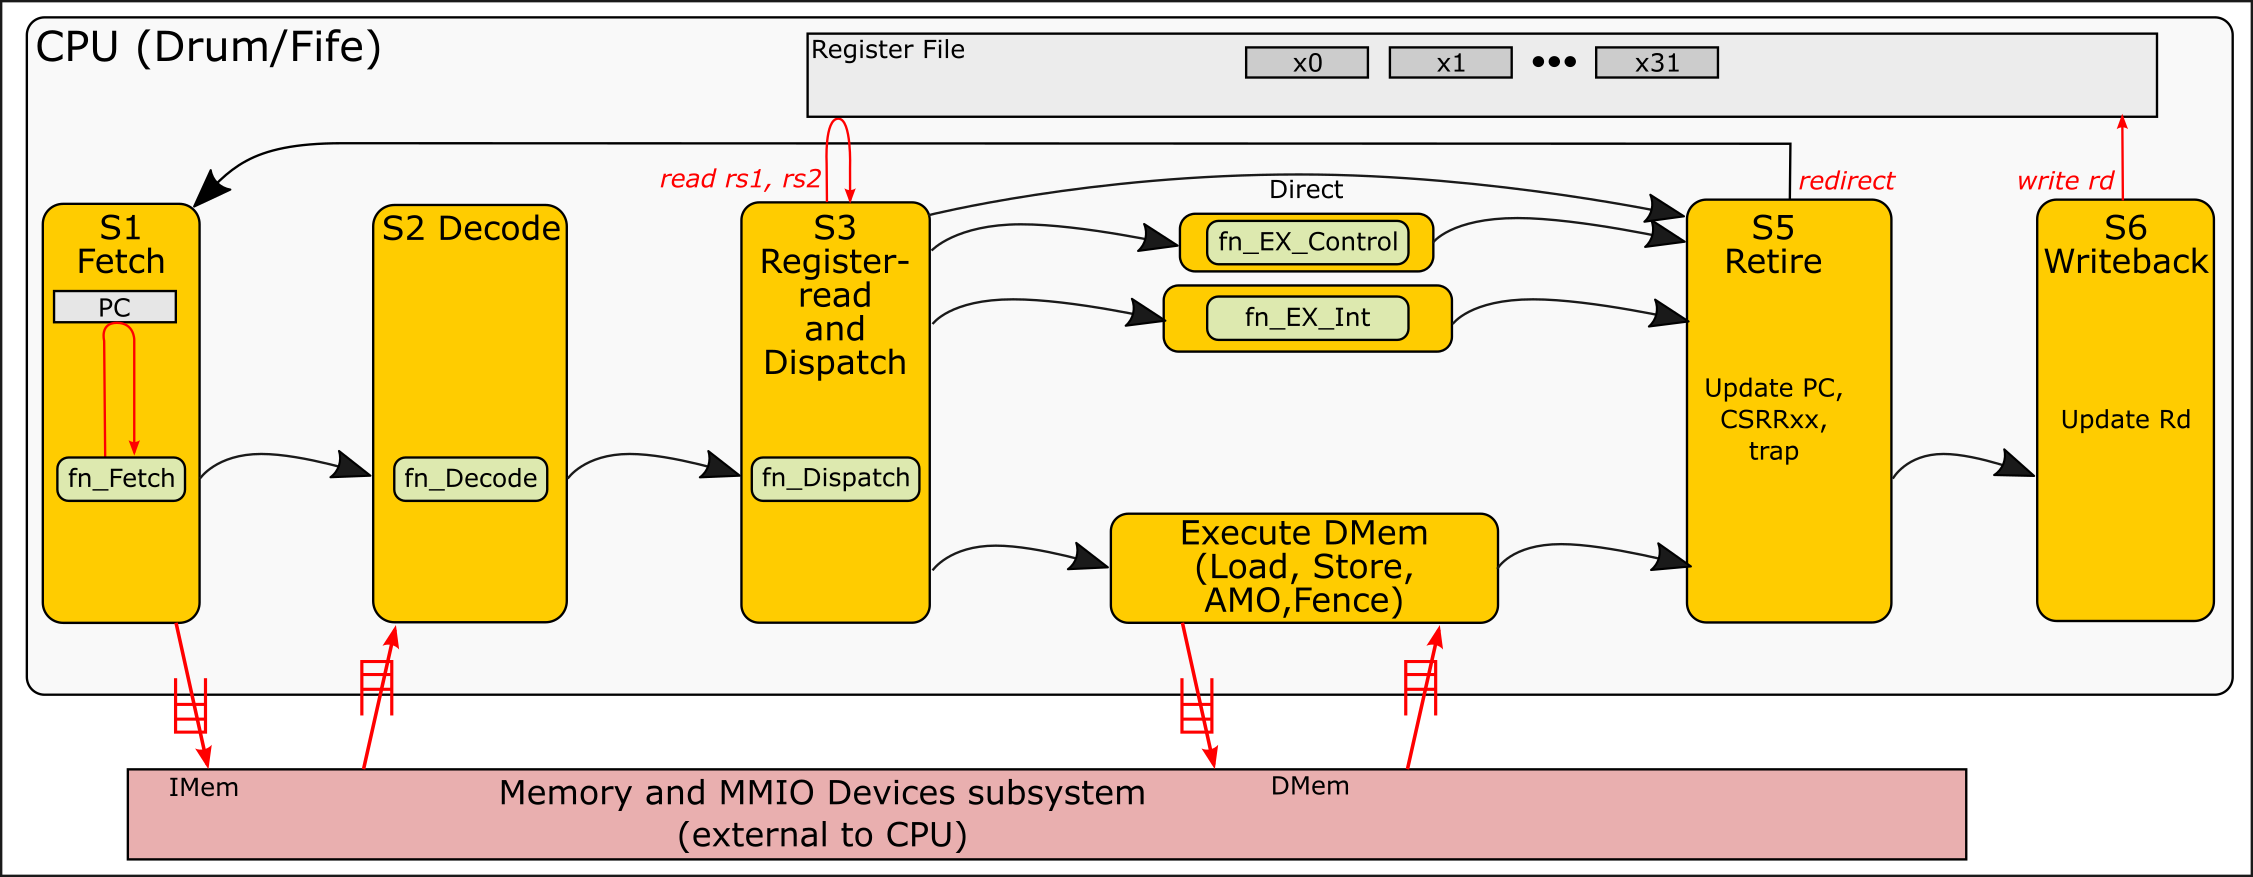
\includegraphics[width=\textwidth]
                  {Figures/RSN_2025-09-01.000.00_FifeDrum_Stages_Multilayer_L1}
 \end{minipage}

 \vspace{1ex}

 \begin{minipage}{0.8\textwidth}\scriptsize
  This diagram illustrates the core steps in executing any instruction.
  The ``{\tt fn\_XXX}'' boxes indicate core functions within each step.

  \vspace*{1ex}

  The ``Memory and MMIO Devices subsystem'' is \emph{external} to the
  CPU and is not our focus today (we will in fact use C code to
  ``model'' this in simulation).  The CPU sends requests to memory;
  for each request and the memory sends a response back to the CPU,
  \emph{after an unknown latency}.  This is an ``asynchronous
  split-phase transaction.''

  \vspace*{1ex}

  Memory-access latency can vary dynamically due to possible caching,
  congestion, varying-length paths to different memory units/devices
  {\etc}.

  \vspace*{1ex}

  The CPU correctness should be robust to this varying latency.

 \end{minipage}
\end{center}

\end{frame}

% ================================================================

\begin{frame}[fragile]
\frametitle{Core pure functions (shared by {\DRUM} and {\FIFE})}

\label{slide_core_functions}

\begin{center}
 \begin{minipage}{0.8\textwidth}\scriptsize
  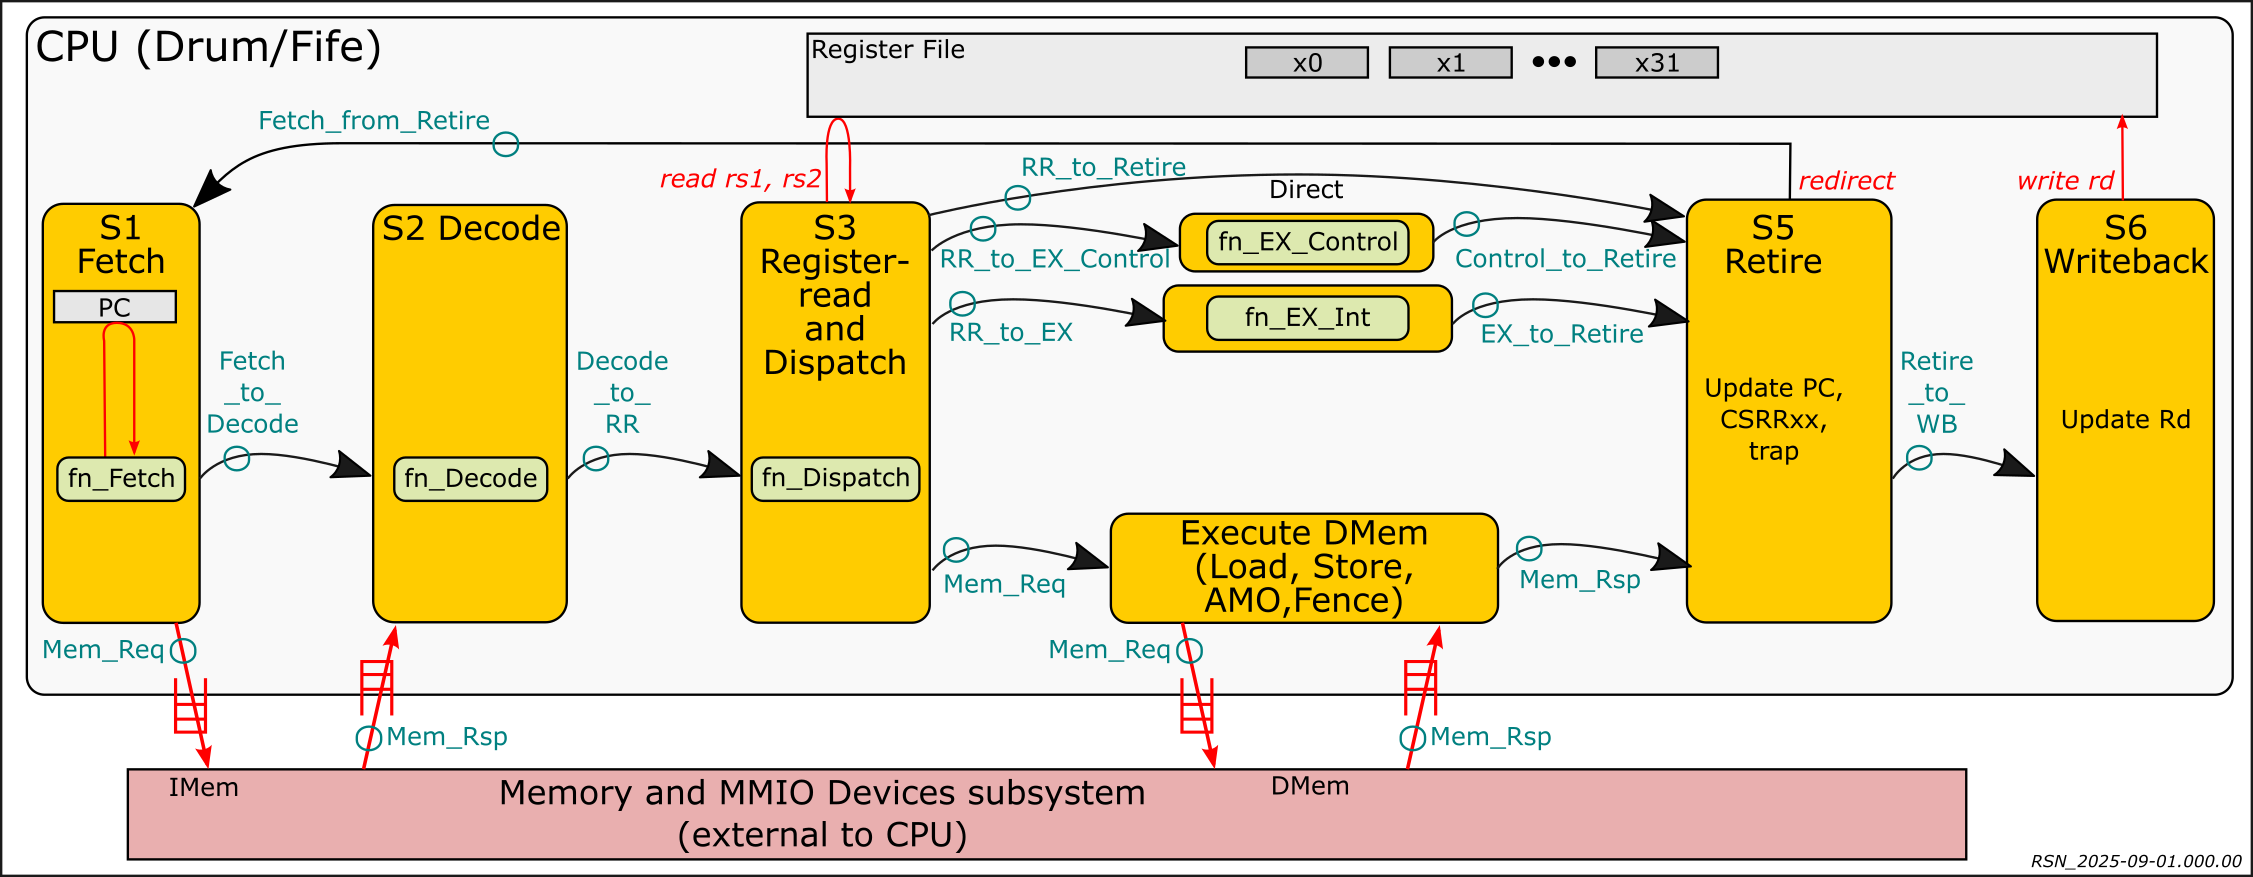
\includegraphics[width=\textwidth]
                  {Figures/RSN_2025-09-01.000.00_FifeDrum_Stages_Multilayer_L1_L3}
 \end{minipage}

 \vspace{1ex}

 \begin{minipage}{0.8\textwidth}\scriptsize

  This diagram annotates each inter-step/stage arrow with the
  ``struct'' type it communicates (in green text).

  \vspace*{1ex}

  The core functions are pure functions, and are shared by {\DRUM} and {\FIFE}:

  \vspace*{1ex}

  {\Eg}
  \fbox{\begin{minipage}{0.8\textwidth}\tiny
   {\tt fn\_Fetch}: (pure) function from the PC to a pair of structs
     of type {\tt Mem\_Req} and {\tt Fetch\_to\_Decode}

   {\tt fn\_Decode}: (pure) function from a pair of structs of type
     {\tt Fetch\_to\_Decode} and {\tt Mem\_Rsp} to a struct of type
     {\tt Decode\_to\_RR}
  \end{minipage}}

  \vspace*{1ex}

  ... and so on.
 \end{minipage}
\end{center}

\end{frame}

% ================================================================

\begin{frame}[fragile]
\frametitle{RISC-V Instruction Encodings}

\begin{center}
 \fbox{
 \begin{minipage}{0.9\textwidth}\scriptsize
  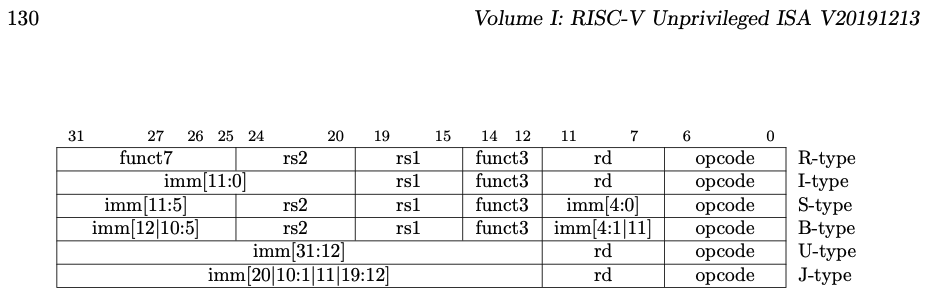
\includegraphics[width=\textwidth]
                  {Figures/Fig_Instr_Encodings.png}
 \end{minipage}}
\end{center}

\end{frame}

% ================================================================

\begin{frame}[fragile]
\frametitle{Let's read some code together: Memory request/response types}

\begin{center}\scriptsize

 \fbox{
  \begin{minipage}{0.9\textwidth}
   \begin{tabbing}
    Repository: \hmm \= {\BookRepo} \hmmmm \\
    File:            \> {\tt Code/src\_Common/Instr\_Bits.bsv} \\
    Focus on:        \> {\tt funct5\_\{LOAD/STORE\}, instr\_funct5()} \\
                     \> {\tt funct3\_\{LB,LH,LW,SB,SH,SW\}, instr\_funct3()}
   \end{tabbing}
  \end{minipage}}

 \vspace*{5ex}

 \begin{minipage}{0.8\textwidth}
  \begin{itemize}

   \item These are the bit-encodings of fields in RISC-V LOAD and
     STORE instructions that indicate whether the instruction is a
     LOAD or a STORE, and whether it is for a Byte (B), Halfword (H),
     Word (W) or doubleword (D).

    \vspace*{2ex}

    These are defined in \emph{The RISC-V Instruction Set Manual
    Volume I, Unprivileged Architecture}, at
    \url{https://drive.google.com/file/d/1uviu1nH-tScFfgrovvFCrj7Omv8tFtkp/view}
    \emph{Chapter 35: RV32/64G Instruction Set Listings}

    \vspace*{5ex}

    {\tiny Other {\tt funct5\_*} definitions are for AMO instructions,
    distinguishing between FETCH and LOAD, {\etc}}

  \end{itemize}

 \end{minipage}
\end{center}

\end{frame}

% ================================================================

\begin{frame}[fragile]
\frametitle{Let's read some code together: struct {\tt Mem\_Req} (memory requests)}

\begin{center}\scriptsize

 \fbox{
  \begin{minipage}{0.9\textwidth}
   \begin{tabbing}
    Repository: \hmm \= {\BookRepo} \hmmmm \\
    File:            \> {\tt Code/src\_Common/Mem\_Req\_Rsp.bsv} \\
    Focus on:        \> struct {\tt Mem\_Req}
   \end{tabbing}
  \end{minipage}}

 \vspace*{5ex}

 \begin{minipage}{0.8\textwidth}
  \begin{itemize}

   \item In struct {\tt Mem\_Req}, the {\tt req\_type} field has type
     {\tt Mem\_Req\_Type}, which is defined earlier in the file to be
     a synonym for {\tt Bit~\#(5)}, {\ie} a 5-bit value, corresponding
     to the {\tt funct5\_*} definitions from the previous slide (LOAD?
     STORE?).

   \item The {\tt req\_size} field has type {\tt Mem\_Req\_Size} which
     is defined earlier in the file as an ``{\tt enum}' type
     indicating whether a memory request is for 1, 2, 4 or 8 bytes.

   \item The {\tt addr} and {\tt data} fields are of type {\tt
     Bit~\#{(64)}}, {\ie} 64-bit wide values.

     The {\tt data} field is only relevant when the request is for a
     STORE instruction; it can be ignored for Fetches, LOADs, and LRs.

     Note: \fbox{\tiny\begin{minipage}{0.8\textwidth}

            We could have used {\tt Bit~\#(XLEN)} for these types,
            where {\tt XLEN} is defined in file {\tt
            Code/src\_Common/Arch.bsv} to be either 32 (for RISC-V
            RV32 implementation) or 64 (for RISC-V RV64
            implementation).  Decoupling the CPU's {\tt XLEN} from the
            memory port width is useful for many reasons:
	    \begin{tightlist}\tiny

              \item A wider memory fetch port allows pre-fetching, and
                    facilitates compressed-instruction parsing.

              \item A wider memory load/store port may be needed for
                    double-precision floating point in an RV32 CPU.

            \end{tightlist}
	   \end{minipage}}

   \item The remaining fields of struct {\tt Mem\_Req} are not
     relevant for the moment.  The {\tt epoch} field is only relevant
     for {\FIFE}, and the remaining fields are only for debugging.

  \end{itemize}

 \end{minipage}
\end{center}

\end{frame}

% ================================================================

\begin{frame}[fragile]
\frametitle{Let's read some code together: struct {\tt Mem\_Rsp} (memory responses)}

\begin{center}\scriptsize

 \fbox{
  \begin{minipage}{0.9\textwidth}
   \begin{tabbing}
    Repository: \hmm \= {\BookRepo} \hmmmm \\
    File:            \> {\tt Code/src\_Common/Mem\_Req\_Rsp.bsv} \\
    Focus on:        \> struct {\tt Mem\_Rsp}
   \end{tabbing}
  \end{minipage}}

 \vspace*{5ex}

 \begin{minipage}{0.8\textwidth}
  \begin{itemize}

   \item The field {\tt rsp\_type} has type {\tt Mem\_Rsp\_Type} which
     is defined earlier in the file to be and {\tt enum} with values
     {\tt MEM\_RSP\_OK}, {\tt MEM\_RSP\_MISALIGNED}, {\tt
     MEM\_RSP\_ERR}, or {\tt MEM\_REQ\_DEFERRED}.

     \vspace{1ex}

     A memory request may succeed, or it may fail because it was
     directed at an unsupported address (``wild'' access), or because
     it was misaligned and the external memory system does not support
     misaligned addresses in requests, or some other reason.  The
     first three response types handle these situations.

     \vspace{1ex}

     {\tt MEM\_REQ\_DEFERRED} can be ignored for now; it is only
     relevant in Fife.

   \item The field \fbox{\tt data} is a 64-bit field containing data in the
   case of a memory access that returns data from memory (FETCH, LOAD,
   AMO).

   \item The remaining fields are only for debugging.

  \end{itemize}

 \end{minipage}
\end{center}

\end{frame}

% ================================================================

\begin{frame}[fragile]
\frametitle{(Repeating earlier diagram, for convenience)}

\begin{center}
 \begin{minipage}{0.8\textwidth}\scriptsize
  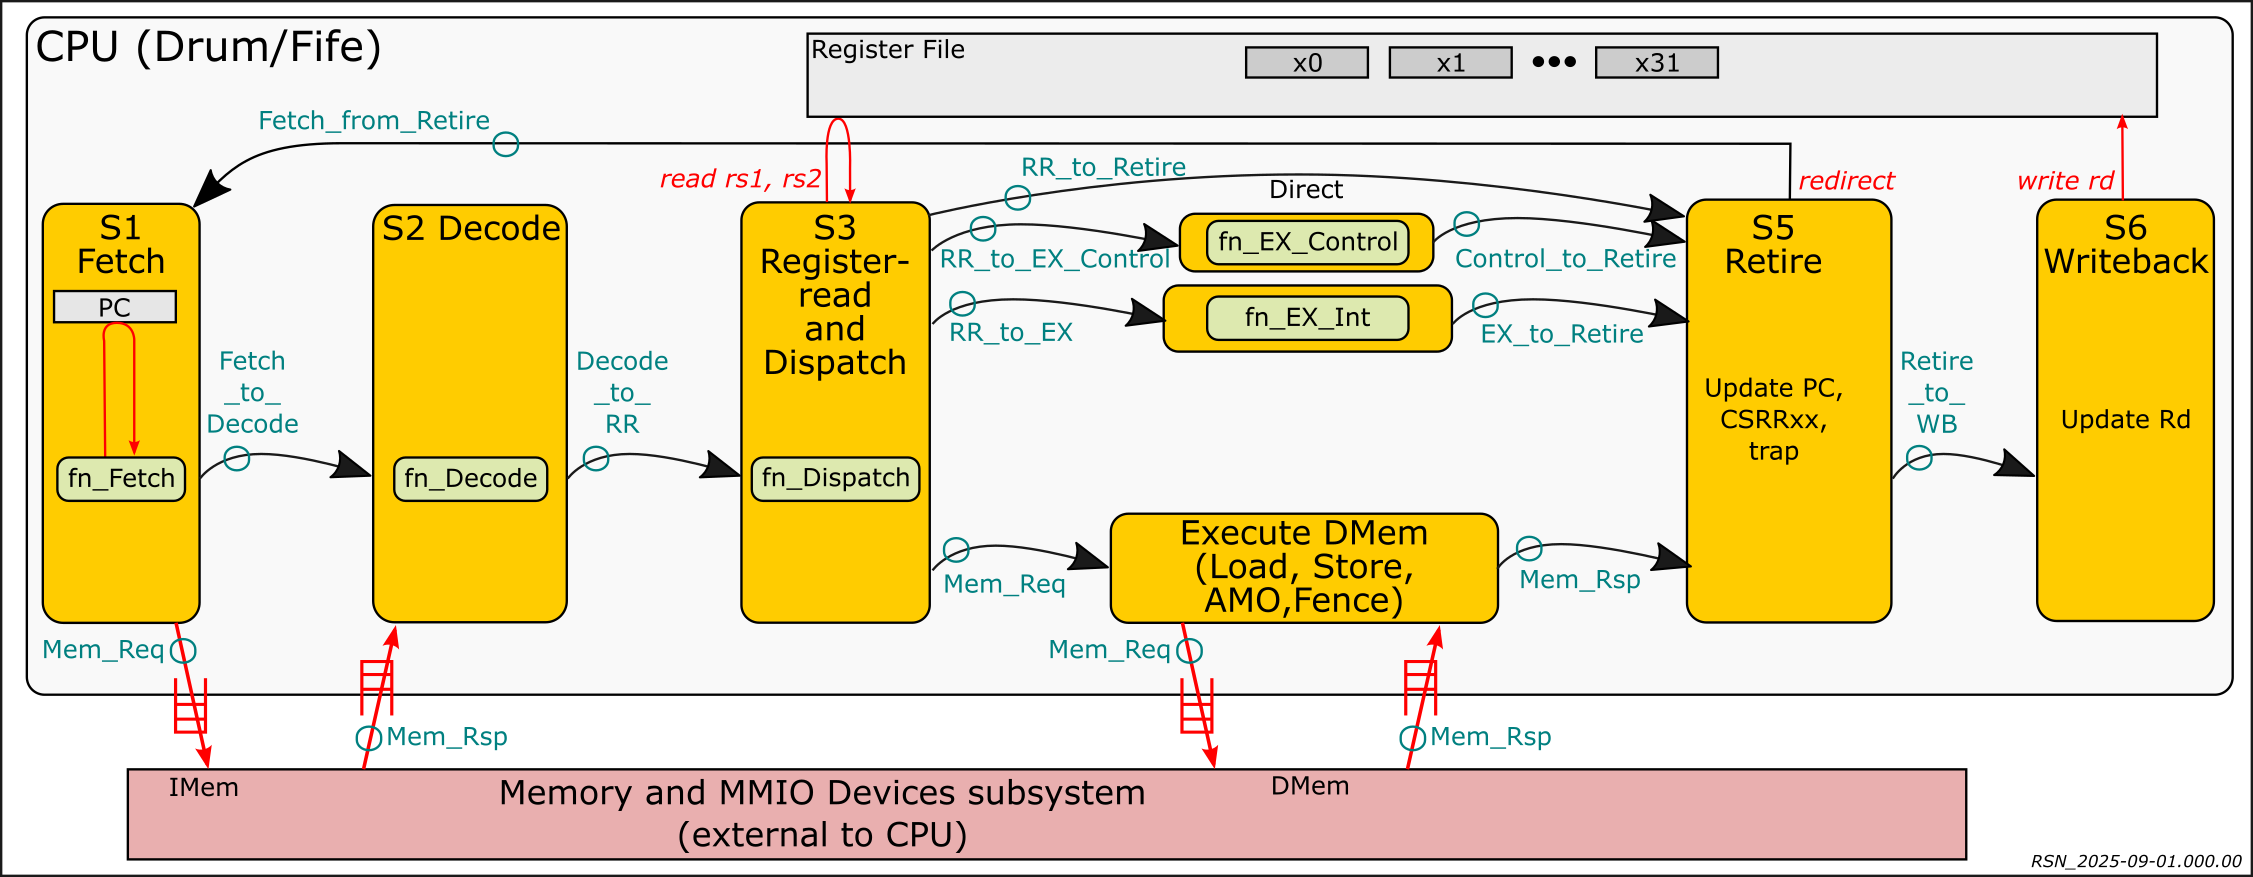
\includegraphics[width=\textwidth]
                  {Figures/RSN_2025-09-01.000.00_FifeDrum_Stages_Multilayer_L1_L3}
 \end{minipage}
\end{center}

\end{frame}

% ================================================================

\begin{frame}[fragile]
\frametitle{Let's read some code together: struct {\tt Fetch\_to\_Decode}}

\begin{center}\scriptsize

 \fbox{
  \begin{minipage}{0.9\textwidth}
   \begin{tabbing}
    Repository: \hmm \= {\BookRepo} \hmmmm \\
    File:            \> {\tt Code/src\_Common/Inter\_Stage.bsv} \\
    Focus on:        \> struct {\tt Fetch\_to\_Decode}
   \end{tabbing}
  \end{minipage}}

 \vspace{1ex}

 \begin{minipage}{0.8\textwidth}
  \begin{itemize}

   \item The notation \fbox{\tt Bit~\#(XLEN)} represents an {\tt XLEN}-wide
     bit-vector.  Parameterization by {\tt XLEN} allows using the same
     code for both RV32 and RV64 implementations.

   \item In the {\tt Fetch\_to\_Decode} struct, the only field of
     interest for the moment is \fbox{\tt pc}, the value of the
     Program Counter. It is forwarded to later steps/stages because:
     \begin{itemize}\scriptsize
      \item It is needed by AUIPC and Branch instructions to compute PC-relative values
      \item It may be needed by JUMP instructions (JAL/JALR) to save a ``return address''
      \item In case of a trap or an interrupt, the PC needs to be saved in the MEPC CSR
     \end{itemize}

   \item The remaining fields ({\tt predicted\_pc}, {\tt epoch}, {\tt
     inum}, {\tt halt\_sentinel}, ...) can be ignored for the
     moment---some are only needed in {\FIFE}, and some are only
     needed for debugger-control.

  \end{itemize}

 \end{minipage}
\end{center}

\end{frame}

% ================================================================

\begin{frame}[fragile]
\frametitle{Let's read some code together: {\tt fn\_Fetch}}

\begin{center}\scriptsize

 \fbox{
  \begin{minipage}{0.9\textwidth}
   \begin{tabbing}
    Repository: \hmm \= {\BookRepo} \hmmmm \\
    File:            \> {\tt Code/src\_Common/Fn\_Fetch.bsv} \\
    Focus on:        \> function {\tt fn\_Fetch}
   \end{tabbing}
  \end{minipage}}

 \vspace{1ex}

 \begin{minipage}{0.8\textwidth}
  \begin{itemize}

   \item Conceptually: {\tt fn\_Fetch: PC} $\rightarrow$ (Memory-request, Info-to-Decode)

   \item Before the function definition is a definition of a struct
     {\tt Result\_F} representing the return-type of the function.  It
     contains a pair of structs of type {\tt Fetch\_to\_Decode} (to be
     sent to the Decode step/stage) and {\tt Mem\_Req} (to be sent to
     memory), respectively.

     Note: \fbox{\begin{minipage}{0.8\textwidth}\tiny
       Unlike C functions, which can only return values of size
       $\leq$ 64 bits, {\BSV} functions can return arbitrarily-wide
       values, including complete structs, vectors, nested structs
       and vectors, {\etc}.
     \end{minipage}}

   \item The return-type of the function {\tt fn\_Fetch} is {\tt
      ActionValue~\#(Result\_F)}. This specifies not only the type of
      the returned value ({\tt Result\_F}), but also that this
      function may have side-effects ({\tt ActionValue~\#()}).  This
      is useful both for user-documentation, but also for the compiler
      (side-effecting functions cannot be optimized as much as
      non-side-effecting (``pure'') functions).

   \item Of the arguments, only {\tt pc} is important, for now. {\tt
     predicted\_pc} and {\tt epoch} are needed in {\FIFE}, and the
     remaining arguments are only for debugging.

   \item The function body is straightforward: it simply creates the
     {\tt Fetch\_to\_Decode} and {\tt Mem\_Req} structs for the
     result.  Note: the memory-request is a LOAD for a 4-byte value (a
     RISC-V instruction) at address {\tt pc}.

     \vspace*{1ex}
     The {\tt zeroExtend} on the address extends 32 bits to 64 bits.
     
  \end{itemize}

 \end{minipage}
\end{center}

\end{frame}

% ================================================================

\begin{frame}[fragile]
\frametitle{(Repeating earlier diagram, for convenience)}

\begin{center}
 \begin{minipage}{0.8\textwidth}\scriptsize
  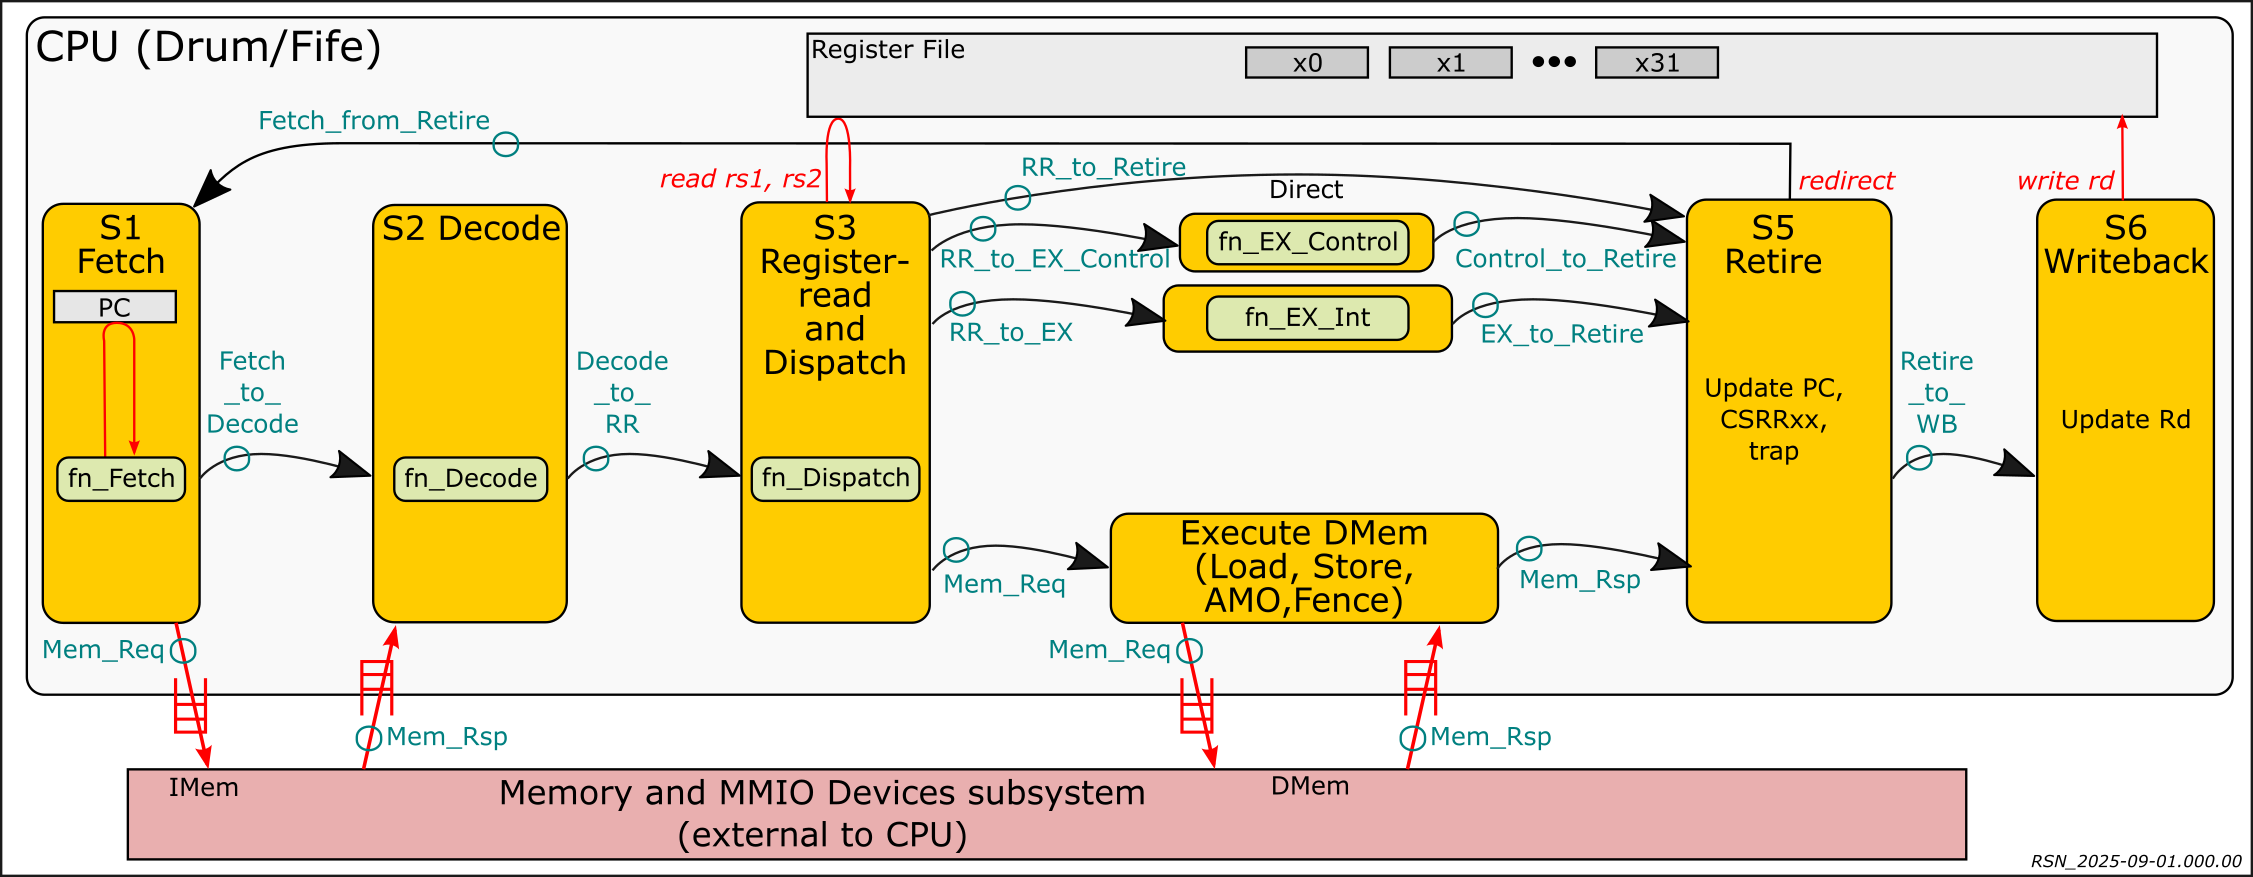
\includegraphics[width=\textwidth]
                  {Figures/RSN_2025-09-01.000.00_FifeDrum_Stages_Multilayer_L1_L3}
 \end{minipage}
\end{center}

\end{frame}

% ================================================================

\begin{frame}[fragile]
\frametitle{Let's read some code together: {\tt fn\_Decode}}

\begin{center}\scriptsize

 \fbox{
  \begin{minipage}{0.9\textwidth}
   \begin{tabbing}
    Repository: \hmm \= {\BookRepo} \hmmmm \\
    Files:           \> {\tt Code/src\_Common/Inter\_Stage.bsv} \\
                     \> {\tt Code/src\_Common/Fn\_Decode.bsv} \\
    Focus on:        \> struct {\tt Decode\_to\_RR}, function {\tt fn\_Decode}
   \end{tabbing}
  \end{minipage}}

 \vspace{1ex}

 \begin{minipage}{0.8\textwidth}
  \begin{itemize}

   \item Conceptually: {\tt fn\_Decode:} (Info-from-Fetch, Memory-response) $\rightarrow$ Info-to-Reg-Read \\
     (refer figure on Slide~\ref{slide_core_functions}).

   \item This step/stage takes the incoming instruction and passes it
     along with some ``classification'' information.  The classes are
     defined as values of the {\tt enum OpClass} type (file {\tt
     Inter\_Stage.bsv}).

     Instructions of the SYSTEM and FENCE classes are sent directly to
     the Retire step/stage.  CONTROL, INT and MEM-class instructions
     are sent into the corresponding fourth-stage execution paths
     shown in the figure on Slide~\ref{slide_core_functions}.

   \item Struct {\tt Decode\_to\_RR} (file {\tt Inter\_Stage.bsv})
     represents the return-type of function {\tt fn\_Decode}.  Some of
     the fields just pass through values that came in on the incoming
     {\tt Fetch\_to\_Decode} struct.

   \item The {\tt has\_rs1}, {\tt has\_rs2} and {\tt has\_rd} are
     booleans indicating whether the instructing reads one or two
     register values, and whether it writes a register value.  The
     {\tt writes\_mem} field is true if the instruction writes to
     memory (STORE, SC, AMO instructions).  The {\tt imm} field is the
     ``immediate'' value from the instruction (different kinds of
     instructions encode immediate values differently).

   \item The {\tt exception} field is true if the Fetch
     memory-response returned a memory error, or if the instruction
     itself is not legal.  In this case, the {\tt cause} and {\tt
     tval} fields provide additional information needed for the trap
     that will be taken in the Retire step/stage.

   \item The {\tt fn\_Decode} function is just a big nested
     conditional that examines the instruction and fills in these
     fields appropriately.  It uses help-functions like {\tt
     is\_legal\_LUI}, {\tt is\_legal\_BRANCH}, and so on, defined in
     {\tt Code/src\_Common/Instr\_Bits.bsv}.

  \end{itemize}

 \end{minipage}
\end{center}

\end{frame}

% ================================================================

\begin{frame}[fragile]

\begin{center}
  {\LARGE Interlude}

 \vspace*{10ex}

 \begin{minipage}{0.9\textwidth}

  {\bf Badger:} \begin{minipage}[t]{0.8\textwidth}
                 Ok, ok, enough of this pseudo-code, I think I get it,
                 but when are we going to start writing the actual hardware code?
		\end{minipage}

  \vspace*{5ex}

  {\bf Owl:} This isn't pseudo-code; this \emph{is} the actual hardware code!

 \end{minipage}

\end{center}

\end{frame}

% ================================================================

\begin{frame}[fragile]
\frametitle{Let's read some code together: \\
            The Register File (General-Purpose Registers, or GPRs) (1/3)}

\begin{center}\scriptsize

 \fbox{
  \begin{minipage}{0.9\textwidth}
   \begin{tabbing}
    Repository: \hmm \= {\BookRepo} \hmmmm \\
    File:            \> {\tt Code/src\_Common/GPRs.bsv} \\
    Focus on:        \> interface {\tt GPRS\_IFC}, module {\tt mkGPRs}
   \end{tabbing}
  \end{minipage}}

 \vspace{1ex}

 \begin{minipage}{0.8\textwidth}
  \begin{itemize}

   \item The RISC-V ISA requires 32 GPRs, where GPR 0 always reads as 0.

   \item {\BSV} designs are composed of \emph{modules}, each of which
     has an \emph{interface}.  These are similar to \emph{objects} and
     \emph{methods} in object-oriented programming languages.

   \item {\tt GPRs\_IFC} defines an interface with several methods.

     \vspace*{1ex}

     {\tt read\_rs1}: this method takes a 5-bit argument {\tt rs1}
     which identifies a GPR, and returns an {\tt xlen}-bit value which
     is the contents of that GPR.  (And, similarly, {\tt read\_rs2}.)

     \vspace*{1ex}

     {\tt write\_rd}: this method takes a 5-bit argument {\tt rs1}
     which identifies a GPR, and an {\tt xlen}-bit argument that is a
     value, and writes that value into that GPR.  The ``return type''
     {\tt Action} indicates that it has a side-effect, and that it
     does not return any value.

   \vspace*{2ex}

   \item {\tt read\_dm}, {\tt write\_dm}: these methods can be ignored
     for now; they are intended for an optional RISC-V Debug Module to
     access registers.

  \end{itemize}

 \end{minipage}
\end{center}

\end{frame}

% ================================================================

\begin{frame}[fragile]
\frametitle{Let's read some code together: \\
            The Register File (General-Purpose Registers, or GPRs) (2/3)}

\begin{center}\scriptsize

 \fbox{
  \begin{minipage}{0.9\textwidth}
   \begin{tabbing}
    Repository: \hmm \= {\BookRepo} \hmmmm \\
    File:            \> {\tt Code/src\_Common/GPRs.bsv} \\
    Focus on:        \> interface {\tt GPRS\_IFC}, module {\tt mkGPRs}
   \end{tabbing}
  \end{minipage}}

 \vspace{1ex}

 \begin{minipage}{0.8\textwidth}
  \begin{itemize}

   \item {\tt mkGPRs} defines a module that presents the {\tt GPRs\_IFC} interfaces.

   \item The first line instantiates the {\BSV} library module {\tt
     mkRegFileFull}; {\tt rf} names the interface to this instance.
     This module has methods {\.sub} to read a register and {\tt .upd}
     to update a register with new value.

   \item The next section initializes all the registers to 0 when
     coming out of reset.  This is not strictly required by the RISC-V
     ISA, but for debugging it is useful to emerge from reset in a
     known state.

     \vspace*{1ex}

     We instantiate a standard {\BSV} library register module {\tt
     mkReg} that is initialized to zero, calling its interface {\tt
     rg\_init\_index}.

     \vspace*{1ex}

     The rule {\tt rl\_init} is effectively a loop, counting up on
     {\tt rg\_init\_index}; at iteration $j$ it writes 0 to GPR[$j$]
     using the {\tt .upd} method for register files.  The rule
     condition (``{\tt (! initialized)}'') specifies when to terminate
     the loop.

     \vspace*{1ex}

     {\tt truncate()} converts the 6-bit {\tt rg\_init\_index} value
     to 5 bits needed for indexes into the register file.  {\BSV} has
     very strict type-checking; there are no silent truncations and
     extensions; without this {\tt truncate()} we'd get a type error.
     
   \item The rest of the module specifies implementations of each method.

     \vspace*{1ex}

     ``{\tt if (initialized)}'' is an \emph{implicit condition} on
     each method, effectively blocking these methods from being
     invoked before complete initialization.

  \end{itemize}

 \end{minipage}
\end{center}

\end{frame}

% ================================================================

\begin{frame}[fragile]
\frametitle{Let's read some code together: \\
            The Register File (General-Purpose Registers, or GPRs) (3/3)}

\begin{center}\scriptsize

 \fbox{
  \begin{minipage}{0.9\textwidth}
   \begin{tabbing}
    Repository: \hmm \= {\BookRepo} \hmmmm \\
    File:            \> {\tt Code/src\_Common/GPRs.bsv} \\
    Focus on:        \> interface {\tt GPRS\_IFC}, module {\tt mkGPRs}
   \end{tabbing}
  \end{minipage}}

 \vspace{1ex}

 \begin{minipage}{0.8\textwidth}
  \begin{itemize}

   \item The rest of the module specifies implementations of each method.

   \vspace*{1ex}

   \item ``{\tt if (initialized)}'' is an \emph{implicit condition} on
       each method, effectively blocking these methods from being
       invoked before complete initialization.

   \item Note that {\tt write\_rd} writes into the register file, but
       in {\tt read\_rs1/rs2}, if the index is zero, they ignore
       what's in the register file and return 0.

       \vspace*{1ex}

       Alternatively, {\tt write\_rd} write 0 if the index is zero,
       and {\tt read\_rs1/rs2} could blindly return the register
       value.

   \vspace*{2ex}

   \item The {\bsc} compiler cannot generate Verilog RTL for module
     {\tt mkGPRs} because it is \emph{polymorphic}---it has interface
     buses of variable width ({\tt xlen}).

     \vspace*{1ex}

     The module {\tt mkGPRs\_synth} fixes the variable {\tt xlen} to
     be the constant {\tt XLEN}.  This module \emph{can} be synthesized
     by {\bsc}.

  \end{itemize}

 \end{minipage}
\end{center}

\end{frame}

% ================================================================

\begin{frame}[fragile]
\frametitle{(Repeating earlier diagram, for convenience)}

\begin{center}
 \begin{minipage}{0.8\textwidth}\scriptsize
  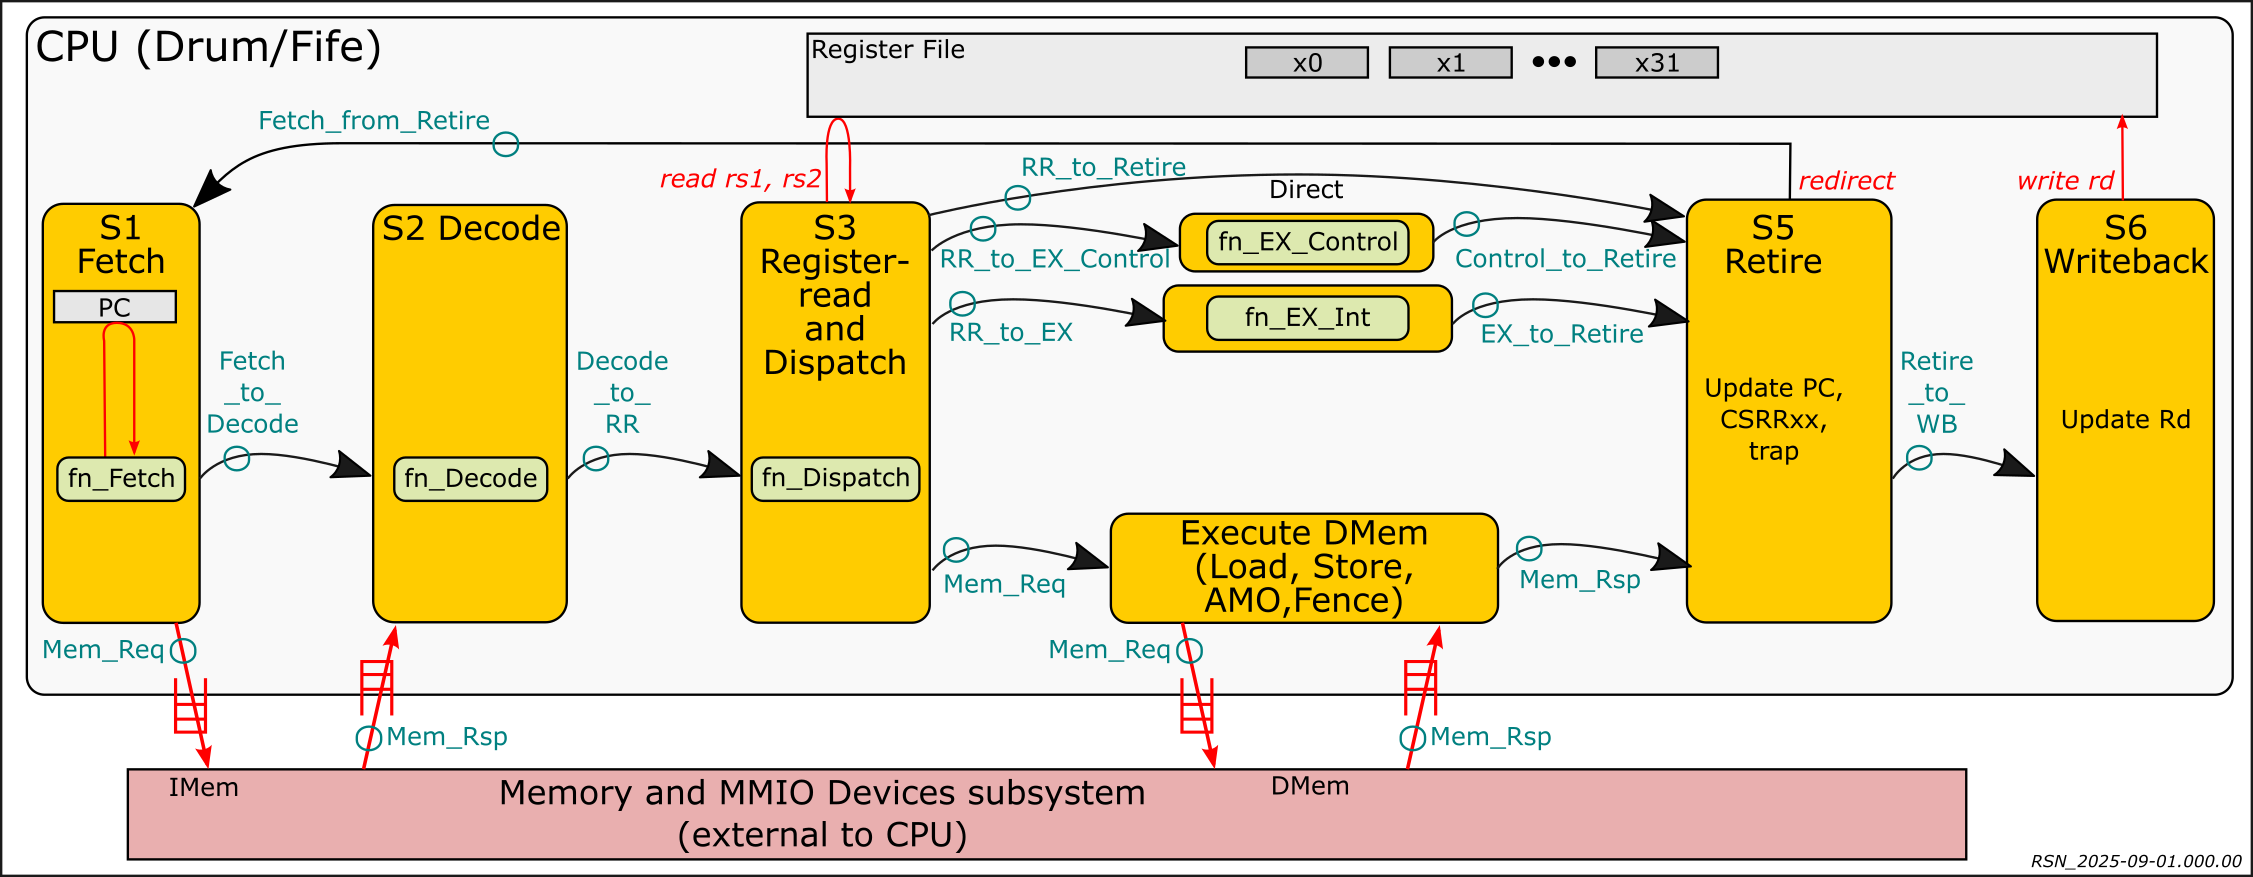
\includegraphics[width=\textwidth]
                  {Figures/RSN_2025-09-01.000.00_FifeDrum_Stages_Multilayer_L1_L3}
 \end{minipage}
\end{center}

\end{frame}

% ================================================================

\begin{frame}[fragile]
\frametitle{Let's read some code together: {\tt fn\_Dispatch}}

\begin{center}\scriptsize

 \fbox{
  \begin{minipage}{0.9\textwidth}
   \begin{tabbing}
    Repository: \hmm \= {\BookRepo} \hmmmm \\
    Files:           \> {\tt Code/src\_Common/Inter\_Stage.bsv} \\
                     \> {\tt Code/src\_Common/Fn\_Dispatch.bsv} \\
    Focus on:        \> structs {\tt RR\_to\_Retire}, {\tt RR\_to\_EX\_Control},  {\tt RR\_to\_EX} \\
                     \> function {\tt fn\_Dispatch}
   \end{tabbing}
  \end{minipage}}

 \vspace{1ex}

 \begin{minipage}{0.8\textwidth}
  \begin{itemize}

   \item Conceptually: {\tt fn\_Dispatch:} Info-from-Decode $\rightarrow$ Info to (Retire, EX\_Control, EX\_Int, EX\_DMem) \\
     (refer figure on Slide~\ref{slide_core_functions}). \\
     The struct type {\tt Result\_Dispatch} contains four sub-structs for this purpose.

   \item Function {\tt fn\_Dispatch()} is straightforward, just
     constucting those four sub-structs and assembling them into the
     result struct.  Each sub-struct is destined for one of the paths
     of execution shown in the figure.

   \item The {\tt RR\_to\_Retire} struct is relevant for every instruction.

   \item The remaining three structs---{\tt RR\_to\_EX\_Control}, {\tt
     RR\_to\_EX}, {\tt RR\_to\_EX\_DMem}---are each relevant only for
     a subset of instructions (Control, Integer and Memory,
     respectively), but this function fills them in blindly; those
     structs/fields will only be examined if relevant, so no harm is
     done if some of the values are bogus.

  \end{itemize}

 \end{minipage}
\end{center}

\end{frame}

% ================================================================

\begin{frame}[fragile]
\frametitle{(Repeating earlier diagram, for convenience)}

\begin{center}
 \begin{minipage}{0.8\textwidth}\scriptsize
  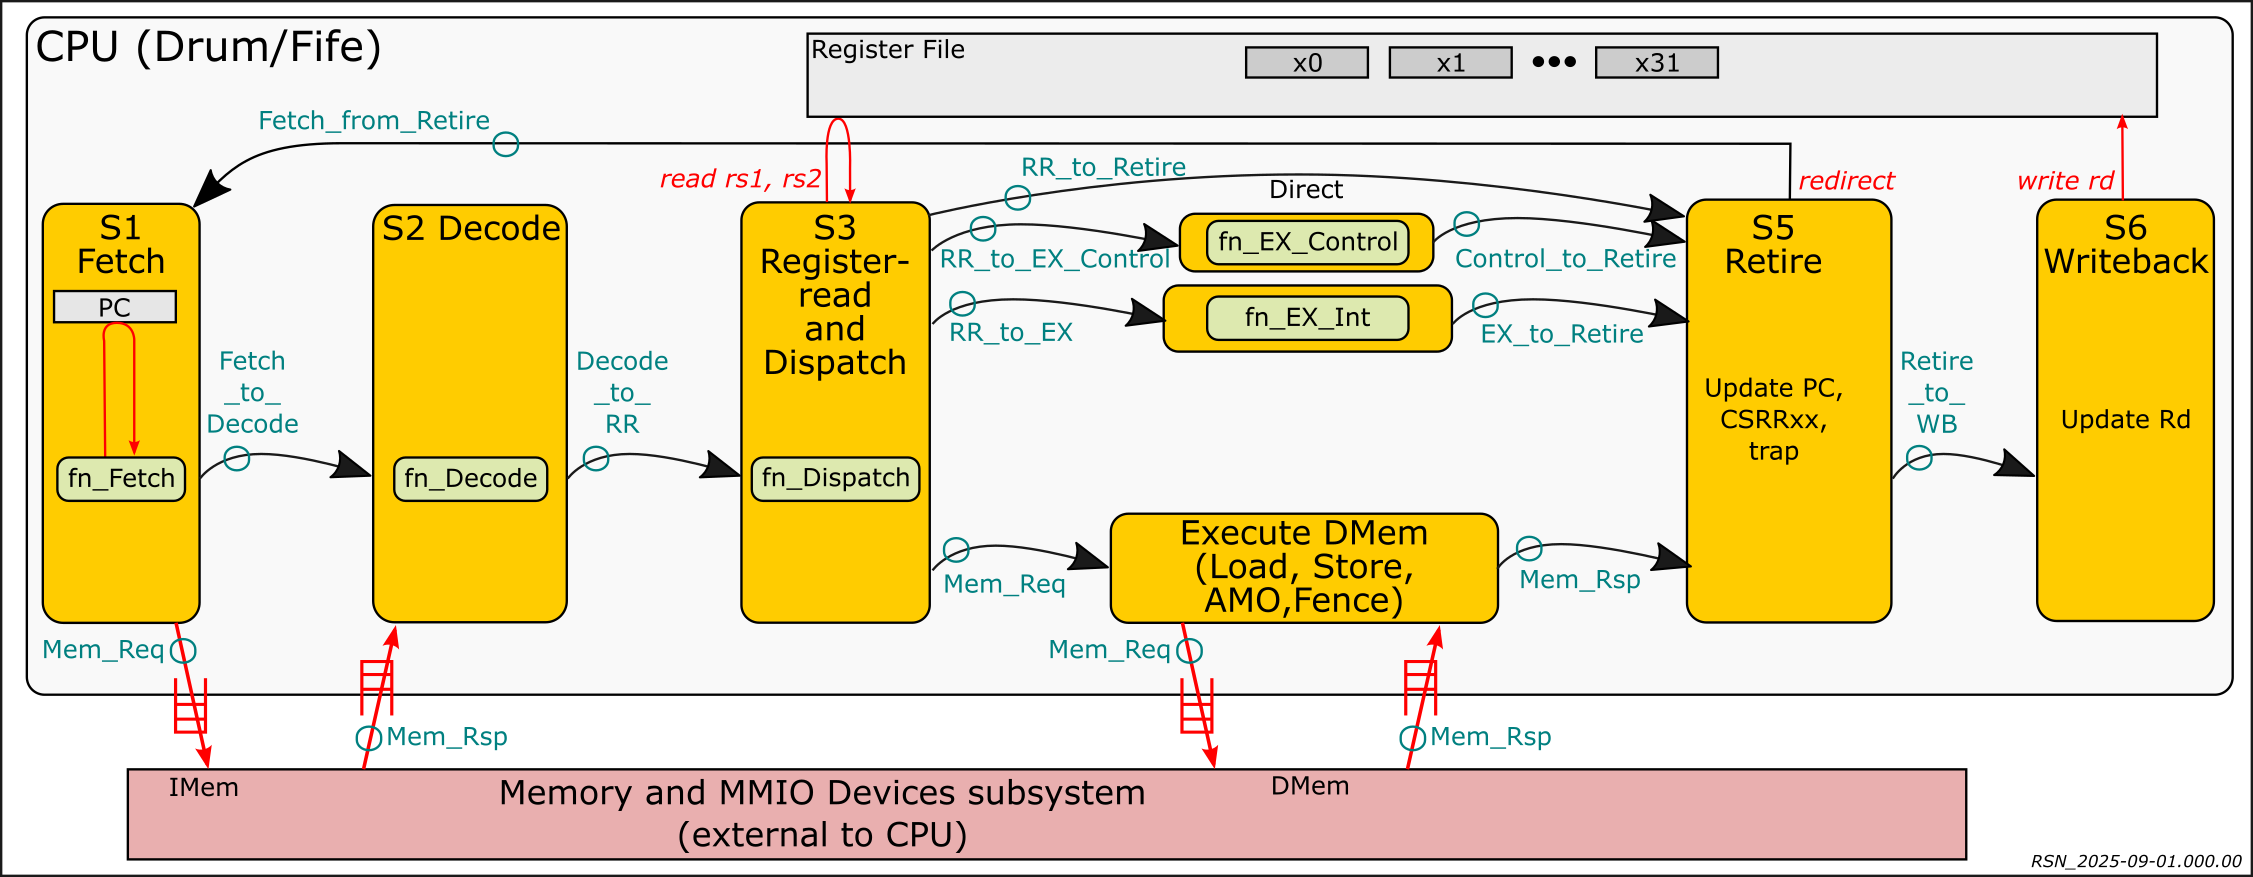
\includegraphics[width=\textwidth]
                  {Figures/RSN_2025-09-01.000.00_FifeDrum_Stages_Multilayer_L1_L3}
 \end{minipage}
\end{center}

\end{frame}

% ================================================================

\begin{frame}[fragile]
\frametitle{Let's read some code together: {\tt fn\_EX\_Control}}

\begin{center}\scriptsize

 \fbox{
  \begin{minipage}{0.9\textwidth}
   \begin{tabbing}
    Repository: \hmm \= {\BookRepo} \hmmmm \\
    Files:           \> {\tt Code/src\_Common/Inter\_Stage.bsv} \\
                     \> {\tt Code/src\_Common/Fn\_EX\_Control.bsv} \\
    Focus on:        \> struct {\tt EX\_Control\_to\_Retire}\\
                     \> function {\tt fn\_EX\_Control}
   \end{tabbing}
  \end{minipage}}

 \vspace{1ex}

 \begin{minipage}{0.8\textwidth}
  \begin{itemize}

   \item Conceptually: {\tt fn\_EX\_Control:} Info-from-Dispatch $\rightarrow$ Info to Retire\\
     (refer figure on Slide~\ref{slide_core_functions}).

   \item Function {\tt fn\_Dispatch()} is straightforward,
     implementing the semantics of RISC-V BRANCH (conditional branch),
     JAL and JALR instructions.

   \item It also checks for misaligned targets.
  \end{itemize}

 \end{minipage}
\end{center}

\end{frame}

% ================================================================

\begin{frame}[fragile]
\frametitle{(Repeating earlier diagram, for convenience)}

\begin{center}
 \begin{minipage}{0.8\textwidth}\scriptsize
  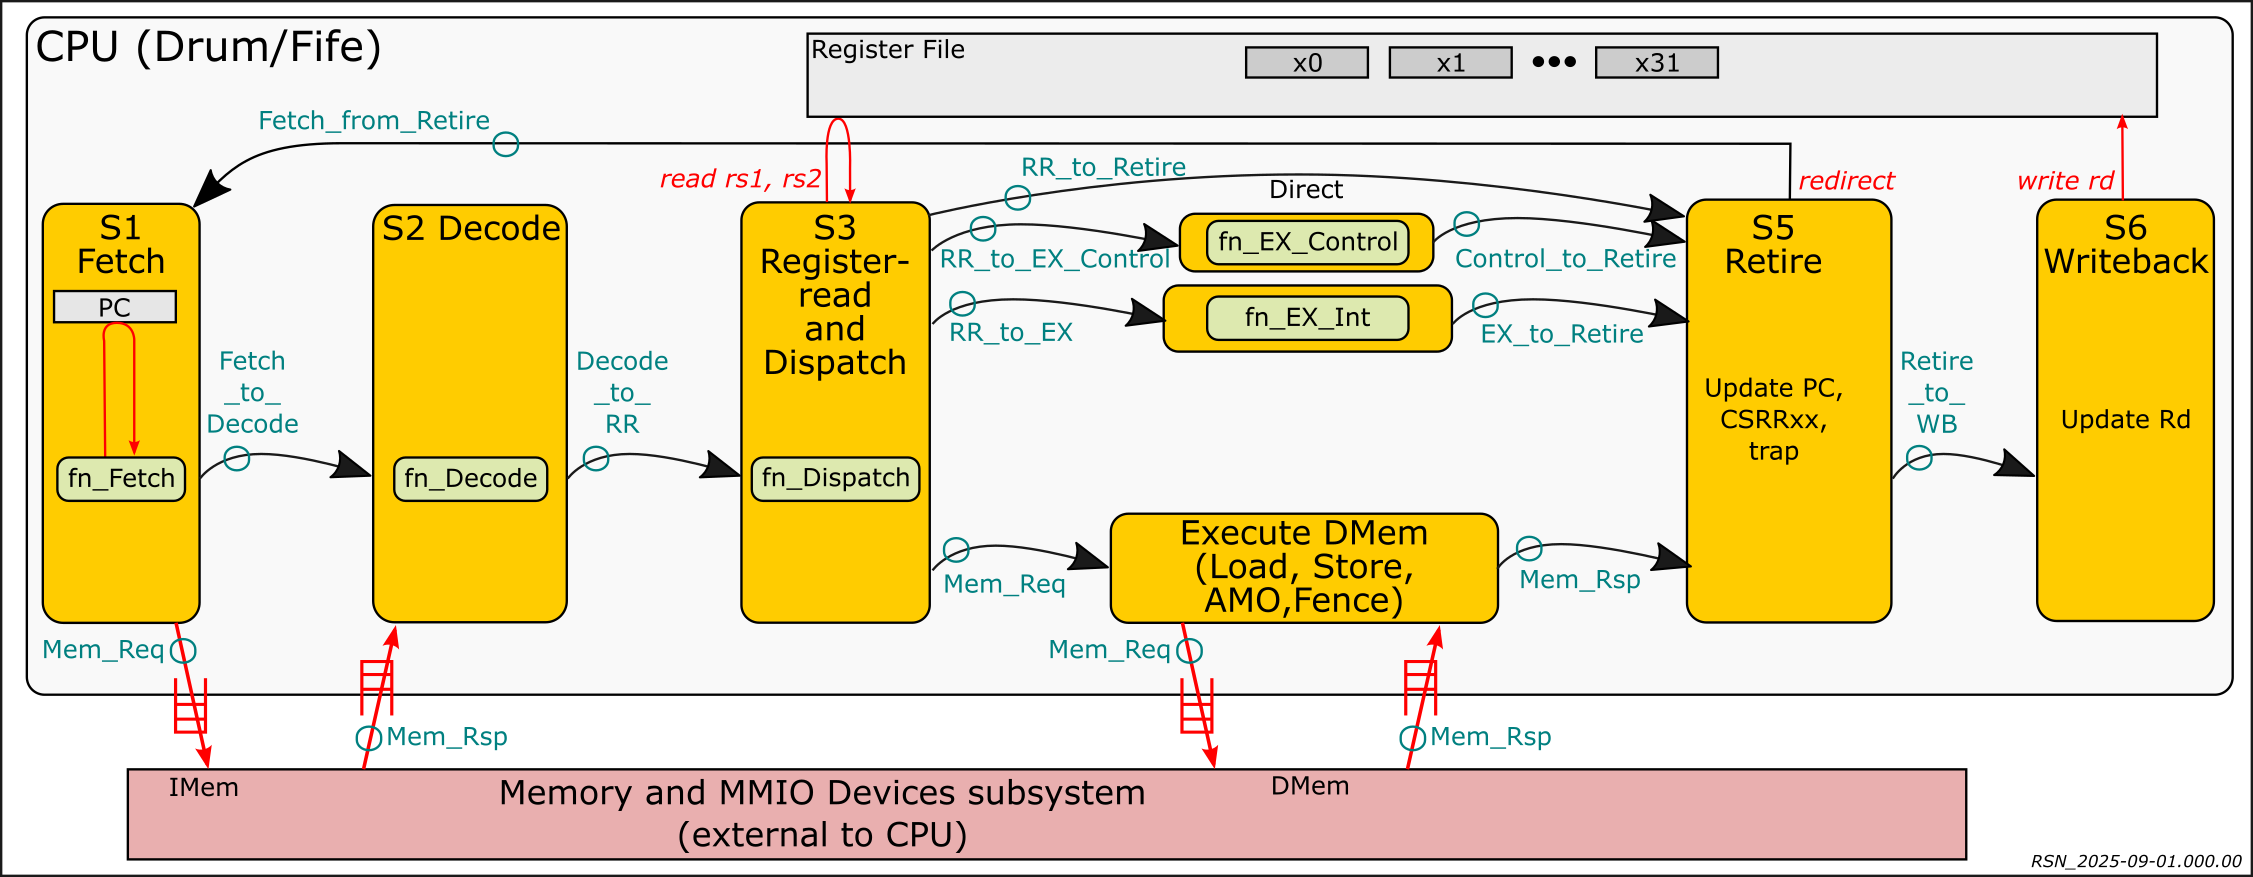
\includegraphics[width=\textwidth]
                  {Figures/RSN_2025-09-01.000.00_FifeDrum_Stages_Multilayer_L1_L3}
 \end{minipage}
\end{center}

\end{frame}

% ================================================================

\begin{frame}[fragile]
\frametitle{Let's read some code together: {\tt fn\_EX\_Int}}

\begin{center}\scriptsize

 \fbox{
  \begin{minipage}{0.9\textwidth}
   \begin{tabbing}
    Repository: \hmm \= {\BookRepo} \hmmmm \\
    Files:           \> {\tt Code/src\_Common/Inter\_Stage.bsv} \\
                     \> {\tt Code/src\_Common/Fn\_EX\_Int.bsv} \\
                     \> {\tt Code/src\_Common/IALU.bsv} \\
    Focus on:        \> struct {\tt EX\_to\_Retire}\\
                     \> function {\tt fn\_EX\_Int} \\
                     \> function {\tt fn\_IALU}
   \end{tabbing}
  \end{minipage}}

 \vspace{1ex}

 \begin{minipage}{0.8\textwidth}
  \begin{itemize}

   \item Conceptually: {\tt fn\_EX\_Int:} Info-from-Dispatch $\rightarrow$ Info to Retire\\
     (refer figure on Slide~\ref{slide_core_functions}).

   \item Function {\tt fn\_Int()} is straightforward,

     implementing the semantics of RISC-V LUI, AUIPC and integer
     operations.  The latter are packaged in function {\tt fn\_IALU},
     which implements the semantics of RISC-V instructions:
     \begin{tabbing}
      \hmm \= (rs1, immed) \hm \= \kill
      \hmm \> (rs1, rs2) \hm   \> ADD, SUB, SLL, SLT, SLTU, SRL, SRA, AND, OR, XOR \\
      \hmm \> (rs1, immed)     \> ADDI, SLTI, SLTIU, ANDI, ORI, XORI, SLLI, SRLI, SRAI
     \end{tabbing}
  \end{itemize}

 \end{minipage}
\end{center}

\end{frame}

% ================================================================

\begin{frame}[fragile]

\begin{center}
  {\LARGE Pause ...}

 \vspace*{10ex}

 \begin{minipage}{0.9\textwidth}

   Modulo minor syntactic differences, these types/functions look like
   types/functions written in many a popular software programming
   language.

   \vspace*{2ex}

   The {\BSV} code gets compiled by the {\bsc} compiler into Verilog.

   \vspace*{10ex}

   And they will be used, as-is, in both {\DRUM} and {\FIFE}.
 \end{minipage}

\end{center}

\end{frame}

% ****************************************************************
% ****************************************************************
% ****************************************************************

\section{\DRUM}

\begin{frame}[fragile]

\frametitle{Contents}

\begin{center}
 \hmm
 \begin{minipage}{0.5\textwidth}
  \tableofcontents
 \end{minipage}
 \hmm
 \begin{minipage}{0.3\textwidth}\scriptsize\it
  \vstrut{0em}{20ex} \\
  \fbox{
   \begin{minipage}{\textwidth}\scriptsize\it
    {\DRUM}
    \begin{tabbing} % Verse
     To temporally sequence the functions \\
     \hmm  Is so easy, almost picayune; \\
     Like writing an ordinary program, \\
     \hmm  A simple FSM; no danger of swoon. \\
     \\
     Before girding up (later) \\
     \hmm  For the pipeline scrum, \\
     Let's FSM our functions and, \\
     \hmm  et voila! We'll have Drum!
    \end{tabbing}
   \end{minipage}}
 \end{minipage}

\end{center}
\end{frame}

% ================================================================

\begin{frame}[fragile]

\begin{center}

  \vstrut{0em}{10ex}

  {\LARGE {\DRUM}: invoking the core pure functions from a sequential Finite State Machine (FSM)}

  \vspace*{5ex}

  This will give us a \emph{hardware implementable} RISC-V CPU:
  \hm {\BSV} $\longrightarrow$ Verilog $\longrightarrow$ FPGA

   \vspace*{5ex}

  \begin{minipage}{0.8\textwidth}
   \begin{itemize}\scriptsize

    \item Not a very fast implementation, but still $\geq 1$
      \emph{order of magnitude} faster than {\BLUESIM} or Verilog
      simulation (boot Linux in minutes instead of days).

    \vspace*{1ex}

    \item Can share the same system-surround (memory, devices) as
      Fife, and run the same software as Fife (because same {\tt
      CPU\_IFC} interface).
    
    \vspace*{1ex}

    \item More ``obviously correct'' than Fife: can be used as a
      verification reference (digital twin) for a more serious
      implementation such as Fife.

    \vspace*{1ex}

    \item More hospitable harness for debugging/verifying functional
      RISC-V parts ({\ie} the non-pipeline parts; the functions we've
      seen so far) than a pipelined CPU

   \end{itemize}
  \end{minipage}

\end{center}

\end{frame}

% ================================================================

\begin{frame}[fragile]
\frametitle{Let's read some code together: {\tt exec\_one\_instr}}

\begin{center}\scriptsize

 \fbox{
  \begin{minipage}{0.9\textwidth}
   \begin{tabbing}
    Repository: \hmm \= {\BookRepo} \hmmmm \\
    Files:           \> {\tt Code/src\_Drum/Drum\_FSM.bsv} \\
    Focus on:        \> {\tt Stmt exec\_one\_instr}
   \end{tabbing}
  \end{minipage}}

 \vspace*{5ex}

 \begin{minipage}{0.8\textwidth}
  \begin{itemize}

   \item ``{\tt exec\_one\_instr}'' is a compound ``statement'' (of type {\tt Stmt}) and is
   a straightforward reading of the steps needed to execute one
   instruction: \\
   \hm Fetch $\rightarrow$ Decode $\rightarrow$ Register-read-and-dispatch
       $\rightarrow$ Execute-and-retire $\rightarrow$ Handle-exception-if-necessary

   \vspace*{1ex}

   \item Each step has been abstracted into an ``action function''
     (such as {\tt a\_Fetch}) which we will study momentarily.

   \vspace*{1ex}

   \item The {\tt seq}-{\tt endseq} bracket indicate that its
     component actions should be performed sequentially (remember,
     {\DRUM} is not pipelined).

   \vspace*{1ex}

   \item The fourth action is itself an if-then-else corresponding to
     the four execution paths on Slide~\ref{slide_core_functions}.
     \\ Some of them use nested {\tt seq}-{\tt endseq} to sequence an
     execute action and a retire action.

  \end{itemize}

 \end{minipage}
\end{center}

\end{frame}

% ================================================================

\begin{frame}[fragile]
\frametitle{Let's read some code together: Execute instructions sequentially, forever}

\begin{center}\scriptsize

 \fbox{
  \begin{minipage}{0.9\textwidth}
   \begin{tabbing}
    Repository: \hmm \= {\BookRepo} \hmmmm \\
    Files:           \> {\tt Code/src\_Drum/Drum\_FSM.bsv} \\
    Focus on:        \> {\tt mk\_AutoFSM}
   \end{tabbing}
  \end{minipage}}

 \vspace*{5ex}

 \begin{minipage}{0.8\textwidth}
  \begin{itemize}

   \item ``{\tt mk\_AutoFSM}'' is a {\BSV} library function that here
     embeds ``{\tt exec\_one\_instr}'' into an infinite loop, thus
     fetching and executing instructions forever (the third arm of the
     if-then-else).

   \vspace*{1ex}

   \item Please ignore the first arm of the if-then-else: that is
     meant for debugger control.

   \vspace*{1ex}

   \item The second arm prioritizes taking an interrupt (if one is
     pending) over executing the next instruction.  Thus, we always
     take interrupts \emph{between} instructions.

  \end{itemize}

 \end{minipage}
\end{center}

\end{frame}

% ================================================================

\begin{frame}[fragile]
\frametitle{(Repeating earlier diagram, for convenience)}

\begin{center}
 \begin{minipage}{0.8\textwidth}\scriptsize
  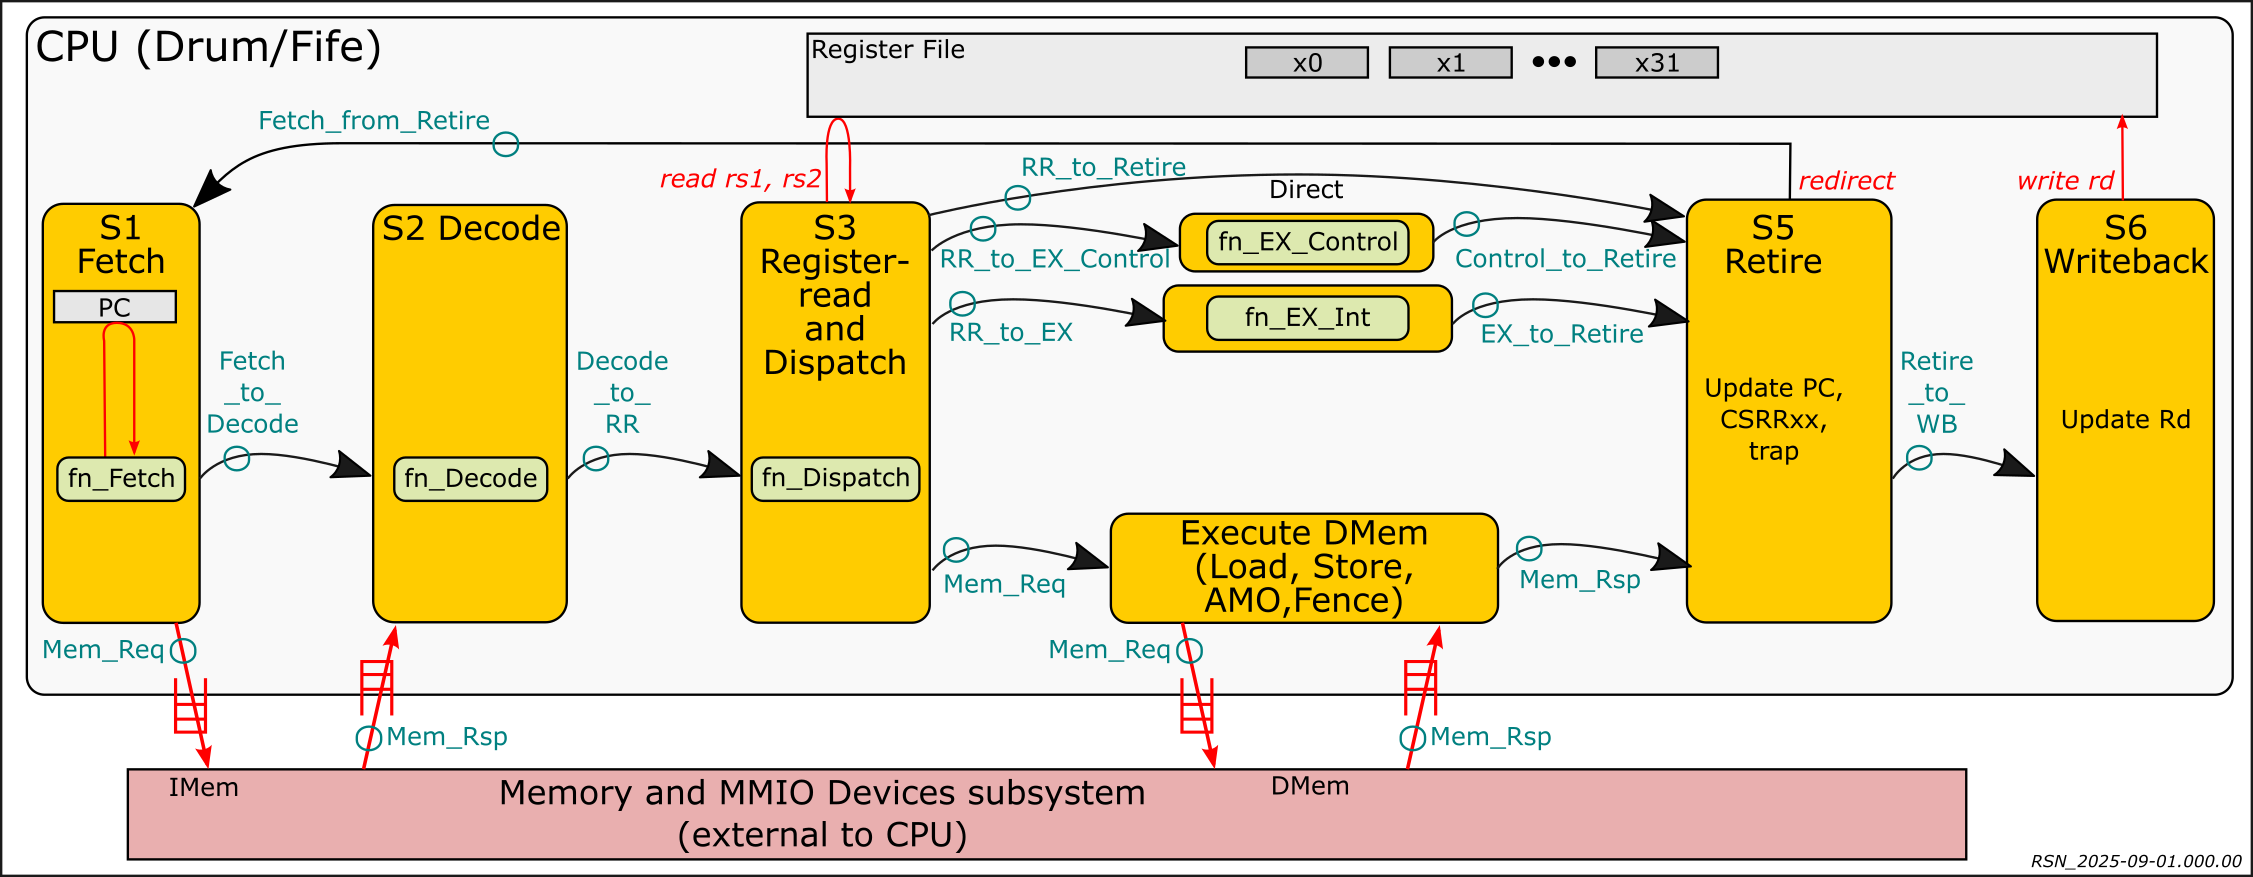
\includegraphics[width=\textwidth]
                  {Figures/RSN_2025-09-01.000.00_FifeDrum_Stages_Multilayer_L1_L3}
 \end{minipage}
\end{center}

\end{frame}

% ================================================================

\begin{frame}[fragile]
\frametitle{Let's read some code together: the interface {\tt CPU\_IFC} for {\FIFE} and {\DRUM}}

\begin{center}\scriptsize
 \fbox{
  \begin{minipage}{0.9\textwidth}
   \begin{tabbing}
    Repository: \hmm \= {\BookRepo} \hmmmm \\
    Files:           \> {\tt Code/src\_Common/CPU\_IFC.bsv} \\
    Focus on:        \> {\tt interface CPU\_IFC}
   \end{tabbing}
  \end{minipage}}

 \vspace*{10ex}

 \begin{minipage}{0.8\textwidth}
  \begin{itemize}

    \item The sub-interface {\tt fo\_IMem\_req}, of type {\tt FIFOF\_O
        \#(Mem\_Req)}, is the output-side of a FIFO to communicate
        instruction-fetch requests to Instruction Memory (IMem).

        \vspace*{1ex}

        The sub-interface {\tt fo\_IMem\_req} is the corresponding
        return path for responses.

    \item The sub-interfaces {\tt fo\_DMem\_req} and {\tt
       fi\_DMem\_rsp} are the corresponding paths to/from Data memory
       (for LOAD/STORE instructions).

    \vspace*{5ex}

    \item ... ignore the remaining sub-interfaces for now; {\eg} the
       sub-interfaces {\tt fo\_DMem\_S\_req} and {\tt
       fi\_DMem\_S\_rsp} are paths to/from Data memory for
       ``speculative'' LOADs and STOREs, and are only relevant for
       {\FIFE}.

  \end{itemize}
 \end{minipage}

\end{center}

\end{frame}

% ================================================================

\begin{frame}[fragile]
\frametitle{Let's read some code together: {\DRUM} CPU state}

\begin{center}\scriptsize

 \fbox{
  \begin{minipage}{0.9\textwidth}
   \begin{tabbing}
    Repository: \hmm \= {\BookRepo} \hmmmm \\
    Files:           \> {\tt Code/src\_Drum/CPU.bsv} \\
    Focus on:        \> {\tt module mkCPU}
   \end{tabbing}
  \end{minipage}}

 \vspace*{5ex}

 \begin{minipage}{0.8\textwidth}
  \begin{itemize}

   \item The CPU state consists primarily of the Program Counter ({\tt
     rg\_pc}), the register file ({\tt gprs}) and the
     Control-and-Status registers ({\tt csrs}).  (Please ignore the
     other registers for now.)

   \vspace*{1ex}

   \item Next, we see the registers holding inter-step values ({\tt
    rg\_Fetch\_to\_Decode} and so on).

    \vspace*{1ex}

    \hm
    \begin{minipage}{0.8\textwidth}
      {\tiny This is a bit extravagant: in our sequential CPU, only
      one of these will be active at time, so we could optimize by
      merging them into a single register capable of holding the
      largest of the inter-stage values, at the expense of clarity.}
    \end{minipage}

   \vspace*{1ex}

   \item Next we see some instantiations of {\BSV} library FIFO
     modules which hold memory requests and responses for Fetch
     (``IMem'') and for LOAD/STORE memory ops (``DMem'').

    \vspace*{1ex}

    \hm
    \begin{minipage}{0.8\textwidth}

      {\tiny This may also seem a bit extravagant: in our sequential
      CPU, we are going to Fetch before LOAD/STORE and vice versa, so
      couldn't we share memory request/response FIFOs?  Yes, but we
      want to keep our interface identical to Fife, where the pipeline
      may simultanously Fetch and LOAD/STORE.}

    \end{minipage}

   \vspace*{1ex}

   \item Next we see some registers to hold information for exceptions
     and traps ({\tt rg\_exception}, {\tt rg\_epc}, {\tt rg\_cause},
     {\tt rg\_tval}).

   \vspace*{1ex}

   \item The next section has registers for debugger control; please
     ignore this for now.

  \end{itemize}

 \end{minipage}
\end{center}

\end{frame}

% ================================================================

\begin{frame}[fragile]
\frametitle{Let's read some code together: {\DRUM} CPU Actions}

\begin{center}\scriptsize

 \fbox{
  \begin{minipage}{0.9\textwidth}
   \begin{tabbing}
    Repository: \hmm \= {\BookRepo} \hmmmm \\
    Files:           \> {\tt Code/src\_Drum/CPU.bsv} \\
    Focus on:        \> {\tt module mkCPU}, section ``Major CPU actions''
   \end{tabbing}
  \end{minipage}}

 \vspace*{5ex}

 The bulk of the module body defines the major CPU action functions
 that we had invoked in the CPU FSM.

 \vspace*{2ex}

 \begin{minipage}{0.8\textwidth}
  \begin{itemize}

   \item Action {\tt a\_Fetch} invokes {\tt fn\_Fetch} (in file {\tt
     src\_Common/Fn\_Fetch.bsv}), passing it the current PC ({\tt
     rg\_pc}).

     \vspace*{1ex}

     The result {\tt y} (of type {\tt Result\_F}, file {\tt
     src\_Common/Fn\_Fetch.bsv}) contains two structs, a
     memory-request, and information for the Decode step.  The former
     is placed in register {\tt rg\_Fetch\_to\_Decode}; the latter is
     enqueued on the FIFO {\tt f\_IMem\_req}.

   \vspace*{1ex}

   \item The remaining functions are similar in flavor, each invoking
     some {\tt fn\_XXXX} function that we have already studied.

   \vspace*{1ex}

   \item Action {\tt a\_Retire\_direct} handles CSRxx, MRET, ECALL,
     EBREAK instructions.

   \vspace*{1ex}

   \item Action {\tt a\_Retire\_DMem} shows how we deal with memory
     exception responses, and responses with data of different sizes
     (Byte, Halfword, Word), with or without sign-extension.

   \vspace*{1ex}

   \item In the final ``interface'' section of the module, a line like: \\
     \hmm {\tt interface fo\_IMem\_req = to\_FIFOF\_O (f\_IMem\_req);} \\
     simply exports the ``output side'' of FIFO {\tt f\_IMem\_req} to the
     CPU interface (sub-interface of {\tt CPU\_IFC}).
  \end{itemize}

 \end{minipage}
\end{center}

\end{frame}

% ================================================================

\begin{frame}[fragile]
\frametitle{Retire actions in {\DRUM}}

 \begin{center}\scriptsize
  \begin{minipage}{0.6\textwidth}\scriptsize
   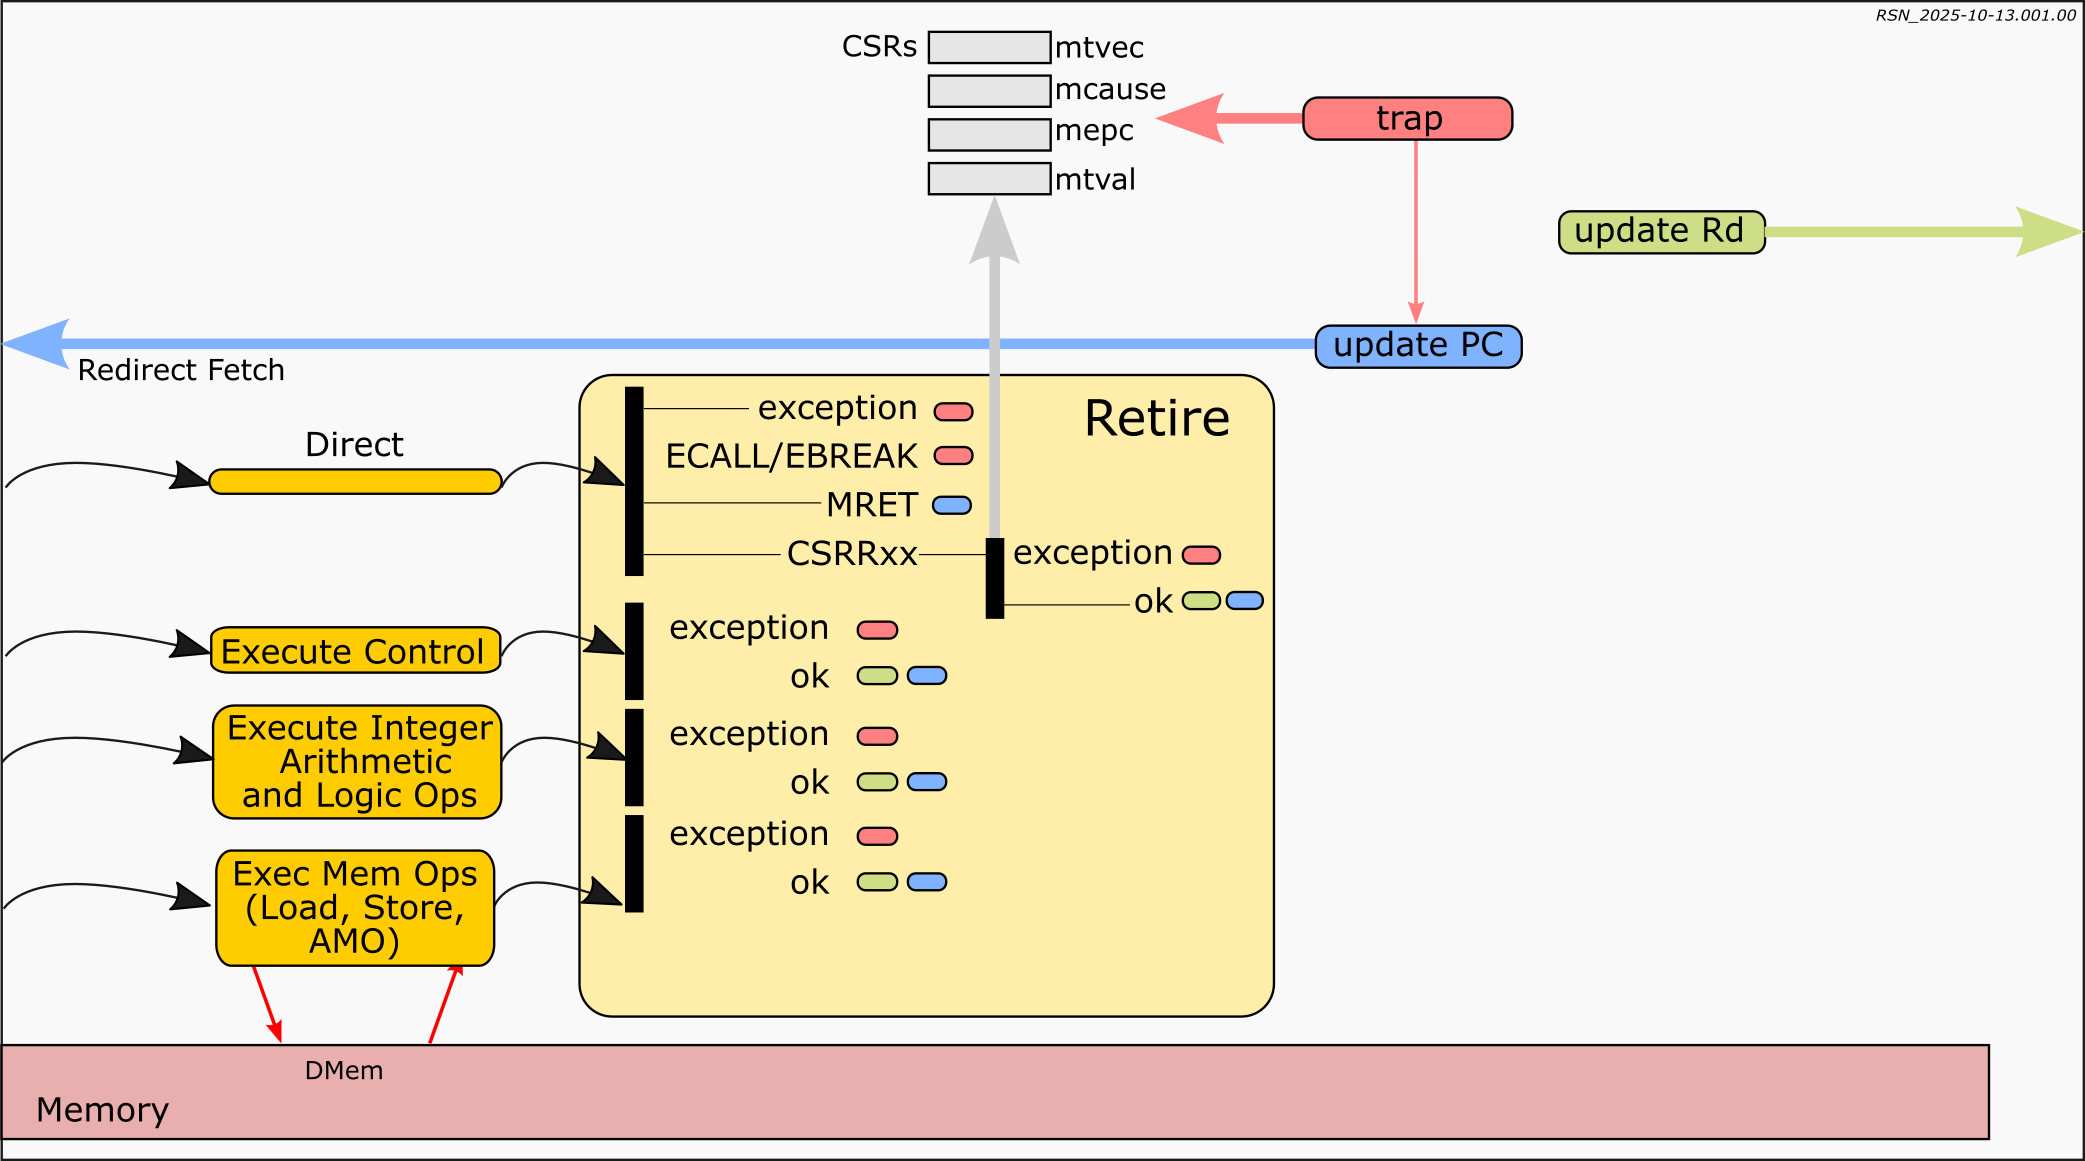
\includegraphics[width=\textwidth]
                   {Figures/RSN_2025-10-13.001.00_Fife_Retire_L1.png}
  \end{minipage}
  \begin{minipage}{0.38\textwidth}
   \begin{itemize}

    \item There are many alternate actions in {\DRUM}'s
          instruction-final retire actions, each taking care of some
          particular situation that preceded retirement.

    \item The rule actions share many common actions, indicated by the
          colored lozenges in the diagram.

   \end{itemize}
   \begin{itemize}\tiny

    \item {\Eg} If the Direct struct indicates a CSRRxx instruction, we
          execute the CSR function. If that raises an exception, we do
          the trap action, else we update Rd and update PC.

    \item {\Eg} If the Direct struct indicates a LOAD/STORE instruction,
          and the DMem response is an exception we do the trap action,
          else we update Rd and update PC.

   \end{itemize}
  \end{minipage}

 \end{center}
\end{frame}

% ================================================================

\begin{frame}[fragile]

\begin{center}
  {\LARGE Pause ...}

 \vspace*{8ex}

 \begin{minipage}{0.8\textwidth}

   ... and we're done reading {\DRUM} code!

   \vspace*{2ex}

   {\scriptsize Modulo minor syntactic differences, it looks like a RISC-V
   simulator program you'd write in many a popular software
   programming language.}

   \vspace*{10ex}

   This code can be compiled to Verilog which, in turn, can be built
   into a Verilog simulation executable, or taken through FPGA or ASIC
   flows into real hardware.

 \end{minipage}

 \vspace*{5ex}

 And that's next on the agenda ...

\end{center}

\end{frame}

% ****************************************************************
% ****************************************************************
% ****************************************************************

\section{{\DRUM}: Generating Verilog, Simulation}

\label{sec_Drum_simulation}

\begin{frame}[fragile]

\frametitle{Contents}

\begin{center}
 \hmm
 \begin{minipage}{0.5\textwidth}
  \tableofcontents
 \end{minipage}
 \hmm
 \begin{minipage}{0.3\textwidth}\scriptsize\it
  \vstrut{0em}{20ex} \\
  \fbox{
   \begin{minipage}{\textwidth}\scriptsize\it
    {\bf {\DRUM}: Generating Verilog, Simulation}
    \begin{tabbing} % Verse
      It's important to take pause \\
      \hmm for instant gratification (some fun), \\
      So let's simulate often, \\
      \hmm it's just a compile-and-run; \\
      \\
      In BSV, like in  OCaml \\
      \hmm and in Haskell before, \\
      If it type-checks and compiles, \\
      \hmm it'll run, for almost sure.
    \end{tabbing}
   \end{minipage}}
 \end{minipage}
\end{center}

\end{frame}

% ================================================================

\begin{frame}[fragile]
\frametitle{The ``CPU-surround'' (shared by {\DRUM} and {\FIFE})}

\begin{center}\scriptsize
 \fbox{
  \begin{minipage}{0.9\textwidth}
   \begin{tabbing}
    Repository: \hmm \= {\BookRepo} \hmmmm \\
    Directory:       \> {\tt Code/src\_Top/} \\
    Files:           \> {\tt Top.bsv}, {\tt Mems\_Devices.bsv}, supporting C files
   \end{tabbing}
  \end{minipage}}

 \vspace*{5ex}

 \begin{minipage}{0.6\textwidth}\scriptsize
  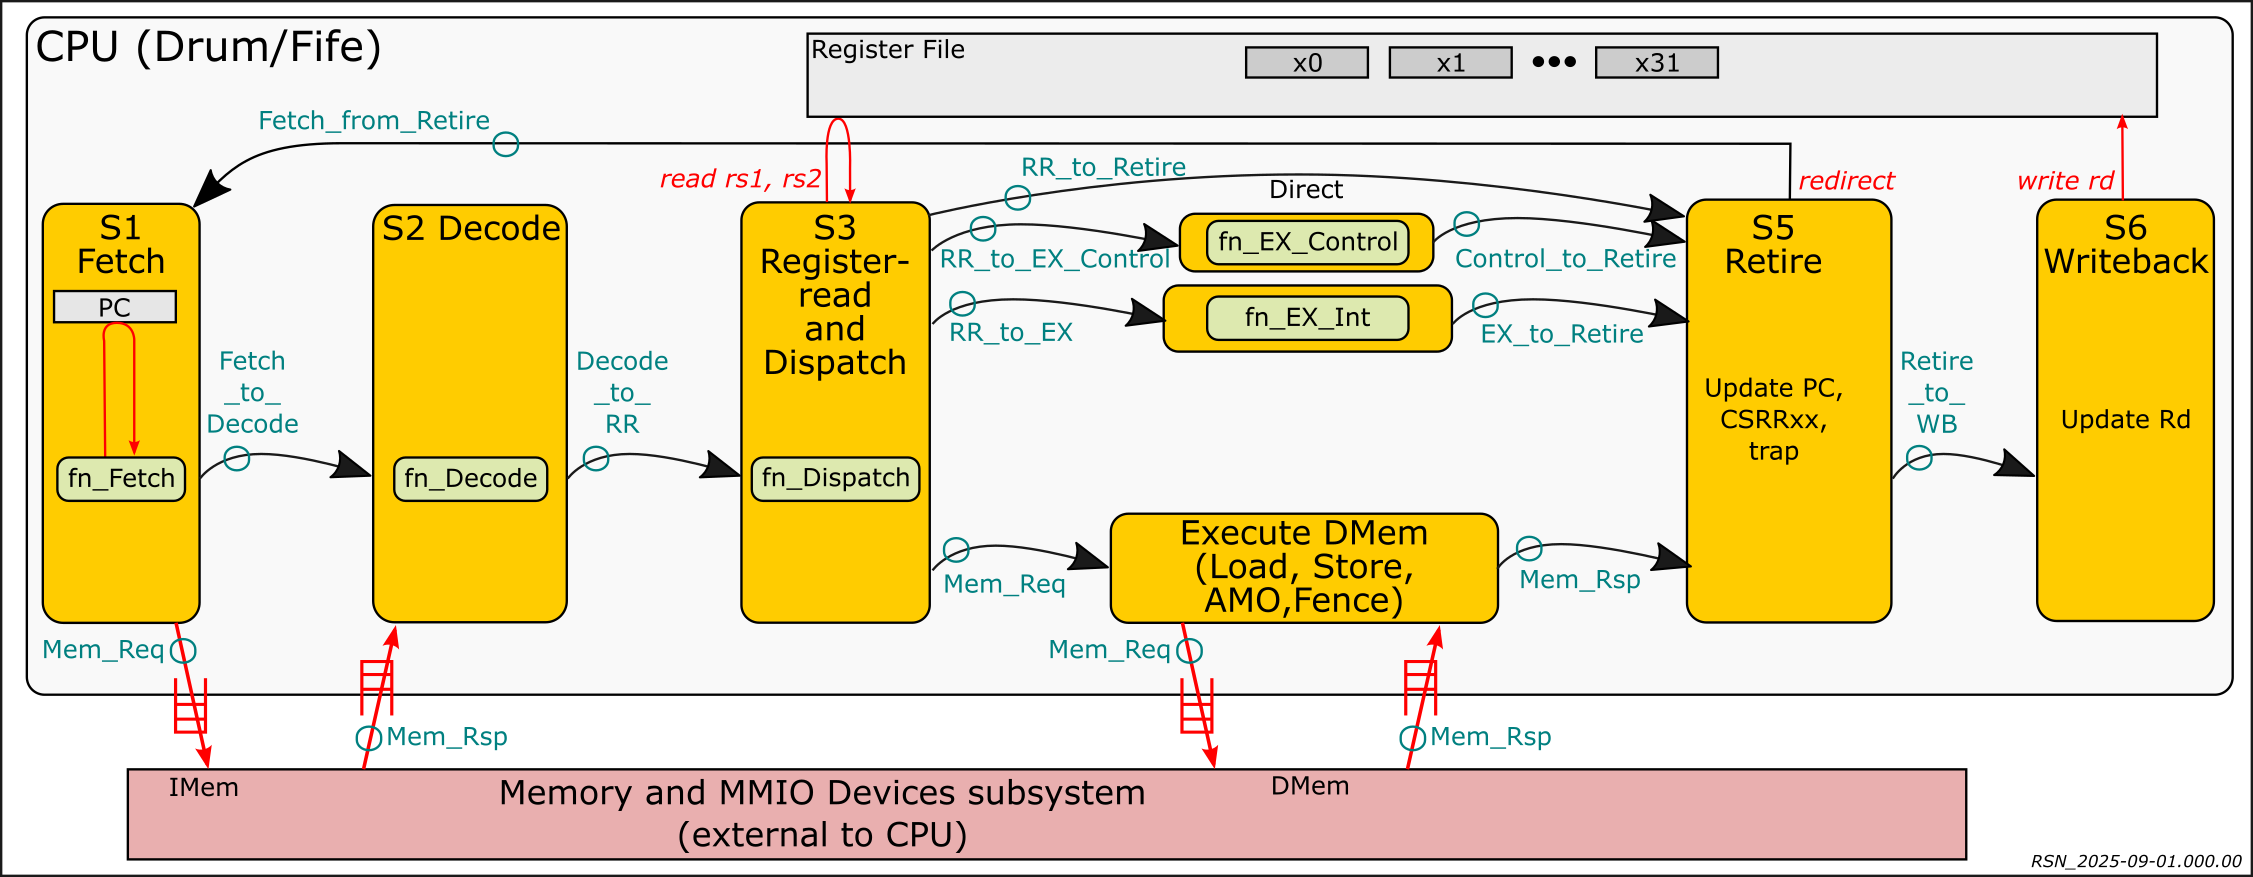
\includegraphics[width=\textwidth]
                  {Figures/RSN_2025-09-01.000.00_FifeDrum_Stages_Multilayer_L1_L3}
% 
\includegraphics[width=\textwidth]{Figures/Fig_Instr_Exec_w_structs.png}
 \end{minipage}
 \hfill
 \begin{minipage}{0.39\textwidth}\scriptsize
  \begin{itemize}

   \item To make a simulation executable we need to connect the CPU
     interfaces to a CPU-surround (the purple box in the diagram).

   \item At a minimum, this should include a memory model

   \item Optional extras include a UART device (for console terminal
     I/O), a timer device (for measuring time and for timer
     interrupts), {\etc}

   \item This code is written in a mixture of {\BSV} and C.

  \end{itemize}
 \end{minipage}
\end{center}

\end{frame}

% ================================================================

\begin{frame}[fragile]
\frametitle{Build Flows for Simulation}

\begin{center}\scriptsize

 \begin{minipage}{0.6\textwidth}\scriptsize
  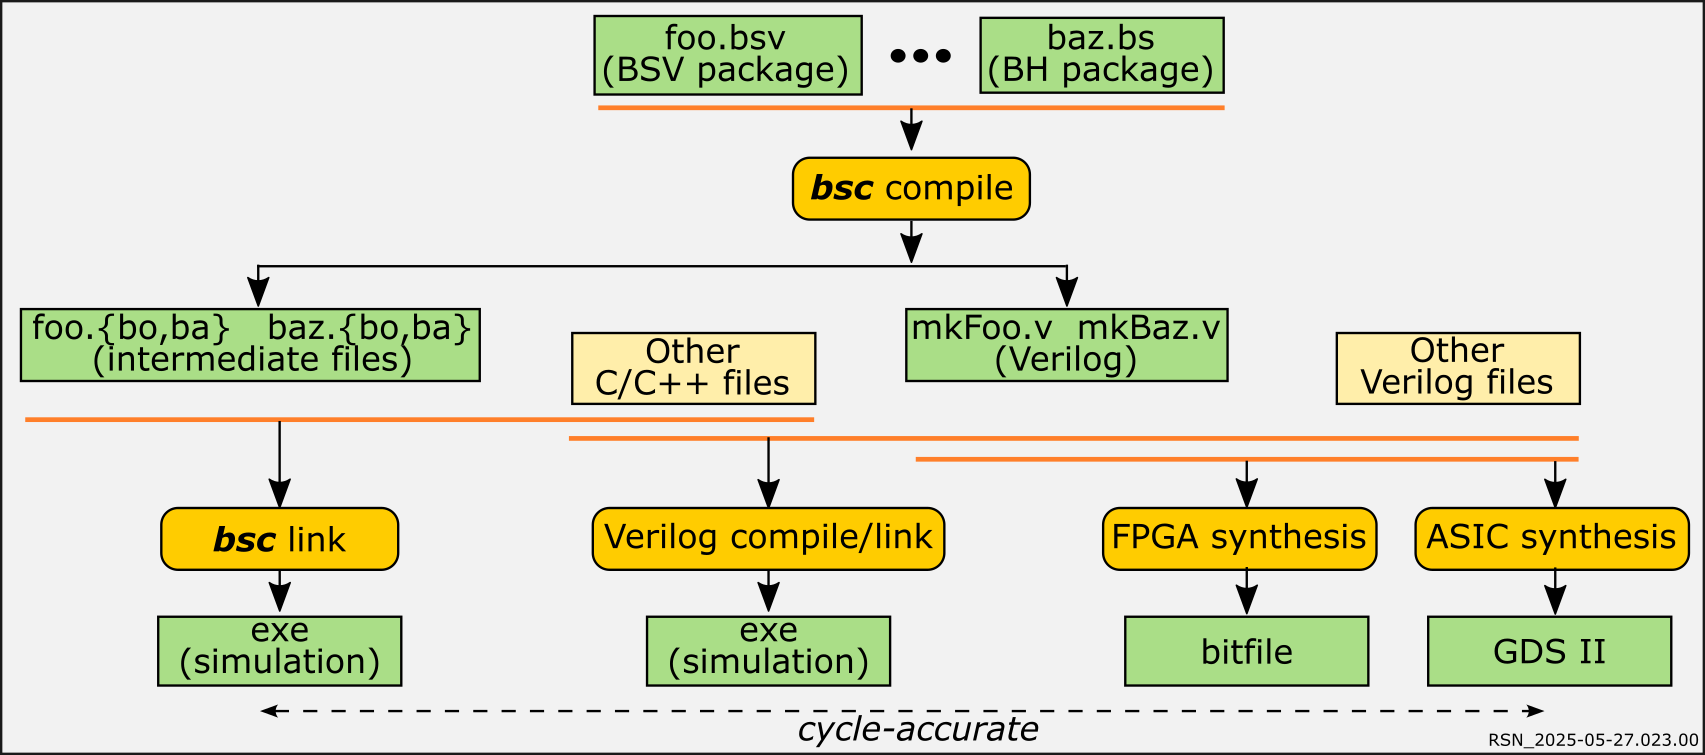
\includegraphics[width=\textwidth]
                  {Figures/RSN_2025-05-27.023.00_BLang_Build_Flows.png}
 \end{minipage}
 \hm
 \begin{minipage}{0.37\textwidth}\scriptsize

  The {\bsc} compiler is typically used in one of two ways, based on command-line flags:
  \begin{itemize}

   \item \emph{either} compile and link {\BSV} into a native-code simulator
         ({\BLUESIM} simulation)

   \item \emph{or} compile {\BSV} into Verilog which can then be run in any
         Verilog simulator.

         \vspace*{1ex}

         {\bsc} can also be used in a second step to link a Verilog
         simulation executable, for many well-known Verilog simulation
         tools (Verilator, Icarus iVerilog, CVC, Verilog simulators
         from Cadence, Synopsys, Siemens, {\etc}).

         \vspace*{1ex}

	 {\tiny The generated Verilog is standard, and can also be processed
	 for FPGA or ASIC (``synthesis'').}

  \end{itemize}

 \end{minipage}
\end{center}

\end{frame}

% ================================================================

\begin{frame}[fragile]
\frametitle{Let's build and run a {\DRUM} simulation, using Bluesim}

\begin{center}\scriptsize

 \fbox{
  \begin{minipage}{0.9\textwidth}
   \begin{tabbing}
    Repository: \hmm \= {\BookRepo} \hmmmm \\
    Directory:       \> {\tt Code/Build/Drum} \\
    Using:           \> {\tt Makefile} (which mostly just ``include''s {\tt ../Include.mk})
   \end{tabbing}
  \end{minipage}}

 \vspace*{2ex}

 \begin{minipage}{0.8\textwidth}
  \begin{itemize}

   \item Let's use the {\bsc} compiler on the {\BSV} sources:

   \hmm\begin{minipage}{0.8\textwidth}\tiny
     \begin{tabbing}\tt
       \$ make b\_compile \\
       bsc -u -sim \hm {\it ... misc {\bsc} flags ...} \\
       \hmm -p   \hm {\it ... directory path where {\bsc} can find source files ...} \\
       \hmm ../../src\_Top/Top.bsv
     \end{tabbing}
   \end{minipage}

   \vspace*{1ex}

   ... creates various intermediate files in the {\tt build\_b/} directory.

   \item Let's use the {\bsc} compiler to link the intermediate files:

   \hmm\begin{minipage}{0.8\textwidth}\tiny
     \begin{tabbing}\tt
       \$ make b\_link \\
       bsc  -sim \hm {\it ... misc {\bsc} flags ...} \\
       \hmm -e mkTop -o ./exe\_Drum\_RV32\_bsim \\
       \hmm  \hm {\it ... misc C files for the CPU-surround} \\
     \end{tabbing}
   \end{minipage}

   \vspace*{1ex}

   ... creates the executable {\tt ./exe\_Drum\_RV32\_bsim}

   \item Let's run the simulation on the famous ``Hello World!''
     program (C, compiled to RISC-V binary):

   \hmm\begin{minipage}{0.8\textwidth}\tiny
     \begin{tabbing}\tt
       \$ make b\_run\_hello \\
       ln -s -f ../../Tools/Hello\_World\_Example\_Code/hello.RV32.bare.memhex32 test.memhex32 \\
       ./exe\_Drum\_RV32\_bsim \\
       {\it ... misc banner material ...} \\
       ================================================================ \\
       Drum v0.81 2024-08-09 (FSM): starting execution at PC 80000000 \\
       ================================================================ \\
       Hello World! \\
       $\uparrow$C
     \end{tabbing}
   \end{minipage}

  \end{itemize}

 \end{minipage}
\end{center}

\end{frame}

% ================================================================

\begin{frame}[fragile]
\frametitle{Let's build and run a {\DRUM} simulation, using Verilog (Verilator)}

\begin{center}\scriptsize

 \fbox{
  \begin{minipage}{0.9\textwidth}
   \begin{tabbing}
    Repository: \hmm \= {\BookRepo} \hmmmm \\
    Directory:       \> {\tt Code/Build/Drum} \\
    Using:           \> {\tt Makefile} (which mostly just ``include''s {\tt ../Include.mk})
   \end{tabbing}
  \end{minipage}}

 \vspace*{2ex}

 \begin{minipage}{0.8\textwidth}
  \begin{itemize}

   \item Let's use the {\bsc} compiler on the {\BSV} sources to generate Verilog:

   \hmm\begin{minipage}{0.8\textwidth}\tiny
     \begin{tabbing}\tt
       \$ make v\_compile \\
       bsc -u -elab -verilog  \hm {\it ... misc {\bsc} flags ...} \\
       \hmm -p   \hm {\it ... directory path where {\bsc} can find source files ...} \\
       \hmm ../../src\_Top/Top.bsv
     \end{tabbing}
   \end{minipage}

   \vspace*{1ex}

   ... generates Verilog files in the {\tt verilog/} directory. \\
   You may wish to peruse this (later, at your convenience).

   \item Let's ask {\bsc} to build a simulation executable (using Verilator):

   \hmm\begin{minipage}{0.8\textwidth}\tiny
     \begin{tabbing}\tt
       \$ make v\_link \\
       bsc -verilog  -vsim verilator  -use-dpi  -vdir verilog \hm {\it ... misc {\bsc} flags ...} \\
       \hmm -e mkTop -o ./exe\_Drum\_RV32\_verilator \\
       \hmm  \hm {\it ... misc C files for the CPU-surround} \\
     \end{tabbing}
   \end{minipage}

   \vspace*{1ex}

   ... creates the executable {\tt ./exe\_Drum\_RV32\_verilator}

   \item Let's run the simulation on the famous ``Hello World!''
     program (C, compiled to RISC-V binary):

   \hmm\begin{minipage}{0.8\textwidth}\tiny
     \begin{tabbing}\tt
       \$ make v\_run\_hello \\
       ln -s -f ../../Tools/Hello\_World\_Example\_Code/hello.RV32.bare.memhex32 test.memhex32 \\
       ./exe\_Drum\_RV32\_verilator \\
       {\it ... misc banner material ...} \\
       ================================================================ \\
       Drum v0.81 2024-08-09 (FSM): starting execution at PC 80000000 \\
       ================================================================ \\
       Hello World! \\
       $\uparrow$C
     \end{tabbing}
   \end{minipage}

  \end{itemize}

 \end{minipage}
\end{center}

\end{frame}

% ****************************************************************
% ****************************************************************
% ****************************************************************

\section{{\FIFE} 6+ stage pipeline}

\begin{frame}[fragile]

\frametitle{Contents}

\begin{center}
 \hmm
 \begin{minipage}{0.5\textwidth}
  \tableofcontents
 \end{minipage}
 \hmm
 \begin{minipage}{0.3\textwidth}\scriptsize\it
  \vstrut{0em}{20ex} \\
  \fbox{
   \begin{minipage}{\textwidth}\scriptsize\it
    {\FIFE} 6+ stage pipeline
    \begin{tabbing} % Verse
      And now let's pipeline it! \\
      \hmm Naive composition would go down flaming; \\
      Order, Prediction, Hazards, Speculation, \\
      \hmm Each issue needs careful taming. \\
      \\
      It's a bit complex; but like many things \\
      \hmm That may initially intimidate, \\
      Once you know how you'll say, "Is that it?", \\
      \hmm Some of all fears will abate.
    \end{tabbing}
   \end{minipage}}
 \end{minipage}
\end{center}

\end{frame}

% ================================================================

\begin{frame}[fragile]
\frametitle{The {\FIFE} pipeline}

\begin{center}\scriptsize
 \begin{minipage}{0.5\textwidth}\scriptsize
  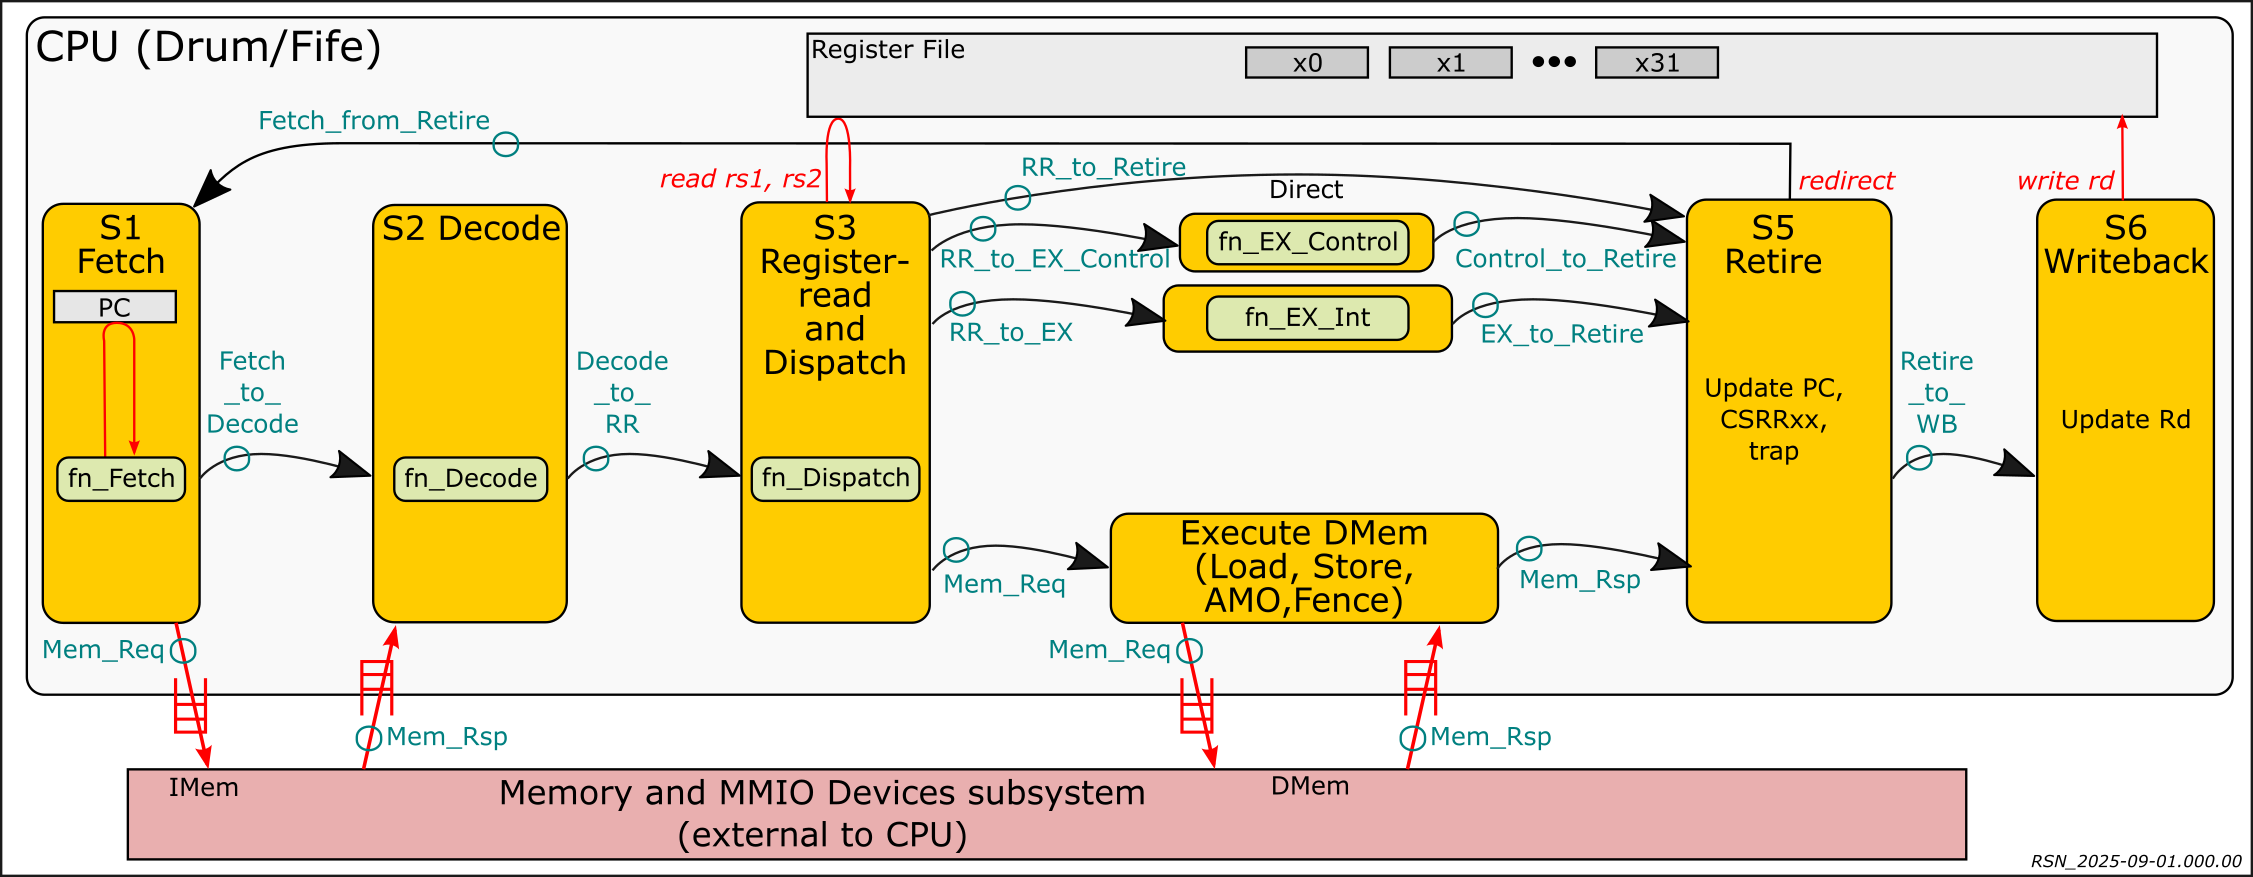
\includegraphics[width=\textwidth]
                  {Figures/RSN_2025-09-01.000.00_FifeDrum_Stages_Multilayer_L1_L3}
 \end{minipage}
 \hfill
 \begin{minipage}{0.49\textwidth}\scriptsize
  In {\DRUM}, this figure represents the sequential states of
     an FSM, {\ie} the steps taken by an FSM, one after the other.
  \begin{itemize}

    \item One instruction is executed completely, going left to right
          through the figure, before we start again on the left,
          for the next instruction.

  \end{itemize}

 \end{minipage}

 \vspace*{2ex}

 \begin{minipage}{0.5\textwidth}\scriptsize
  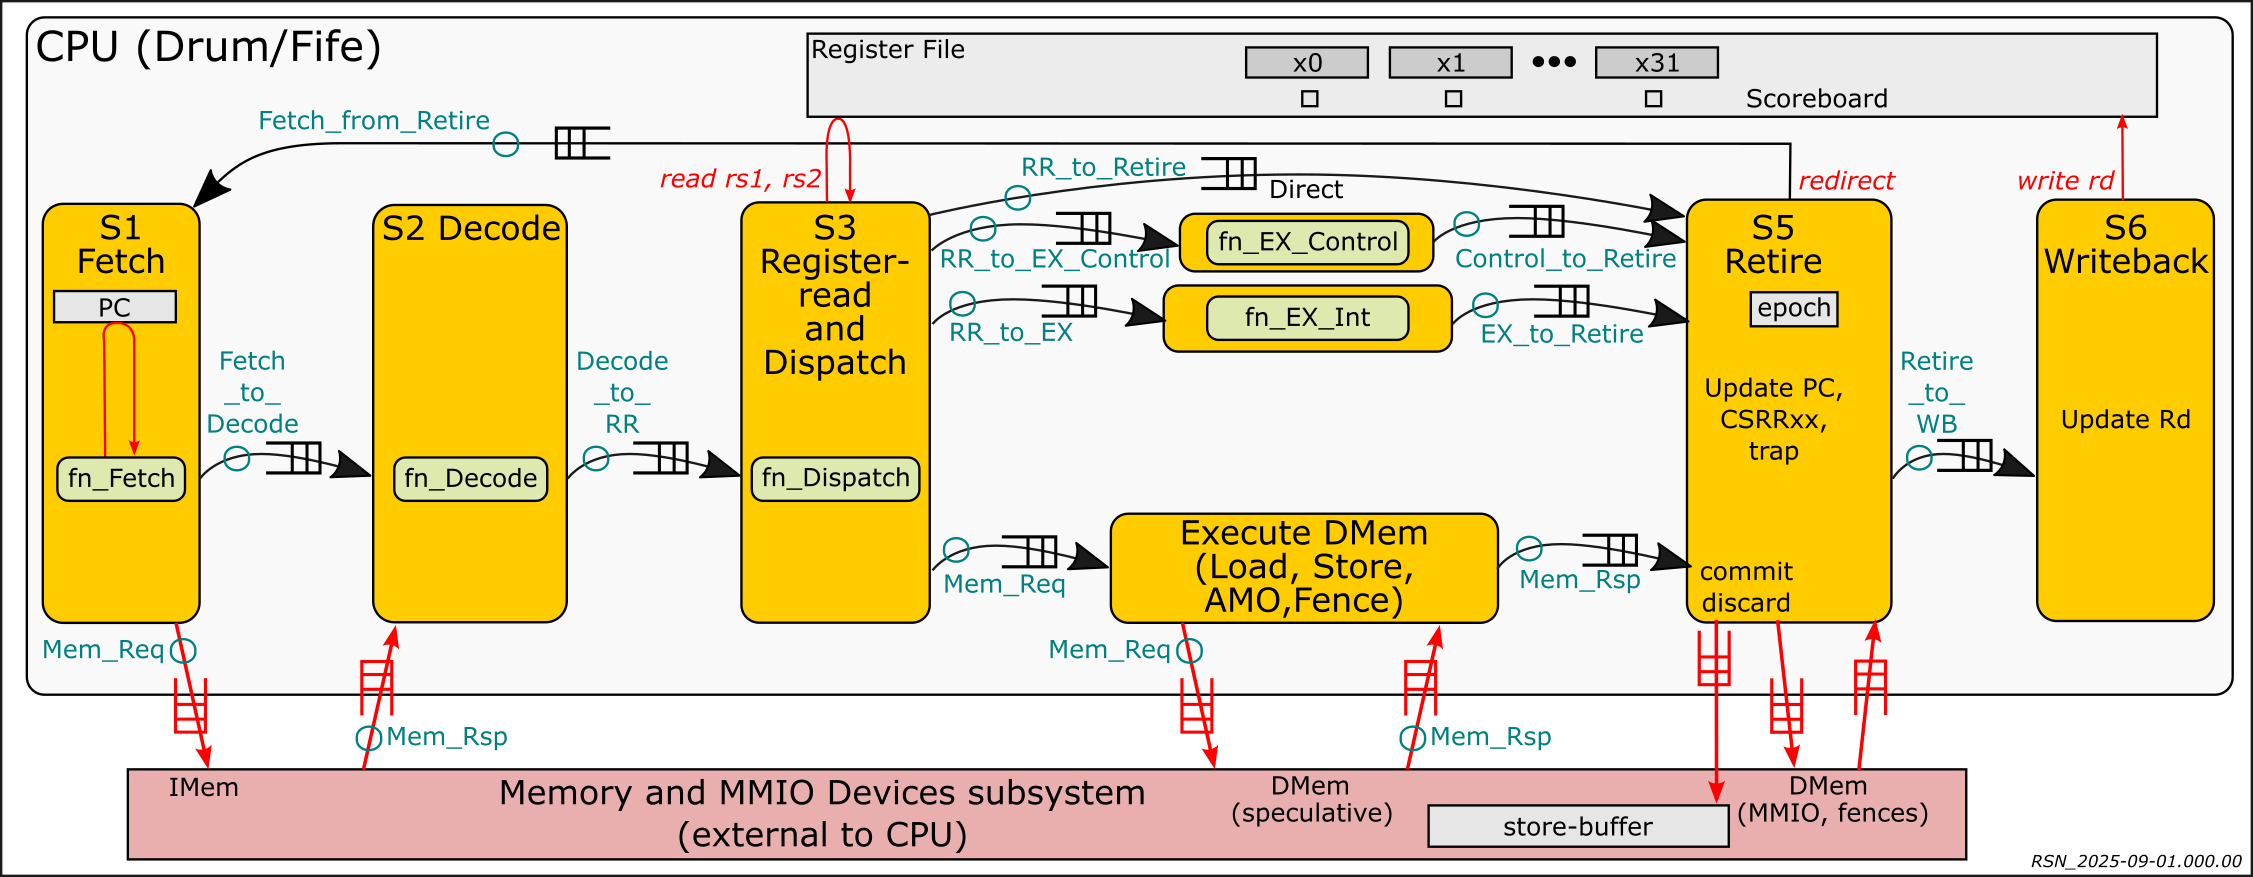
\includegraphics[width=\textwidth]
                  {Figures/RSN_2025-09-01.000.00_FifeDrum_Stages_Multilayer_L1_L2_L3}
 \end{minipage}
 \hfill
 \begin{minipage}{0.49\textwidth}\scriptsize
  In {\FIFE}, this same figure represents a \emph{pipeline}:
  \begin{itemize}
    \item Each module (Fetch, Decode, ...) is an infinite
          \emph{process}, and they all run concurrently.  Each is
          called a ``pipeline stage''.

    \item All connections between modules are now FIFOs.

    \item Instructions ``stream'' through the figure, from left
          to right.

    \item At any given point in time, there could be several
       instructions ``in flight'', in the various stages, in various
       states of completion.

  \end{itemize}
 \end{minipage}

 \vspace*{3ex}

 {\normalsize {\bf NOTE:} {\FIFE} invokes exactly the same core pure functions as {\DRUM}}

\end{center}

\end{frame}

% ================================================================

\begin{frame}[fragile]
\frametitle{The {\FIFE} pipeline: new concerns}

\begin{center}\scriptsize
 \begin{minipage}{0.5\textwidth}\scriptsize
  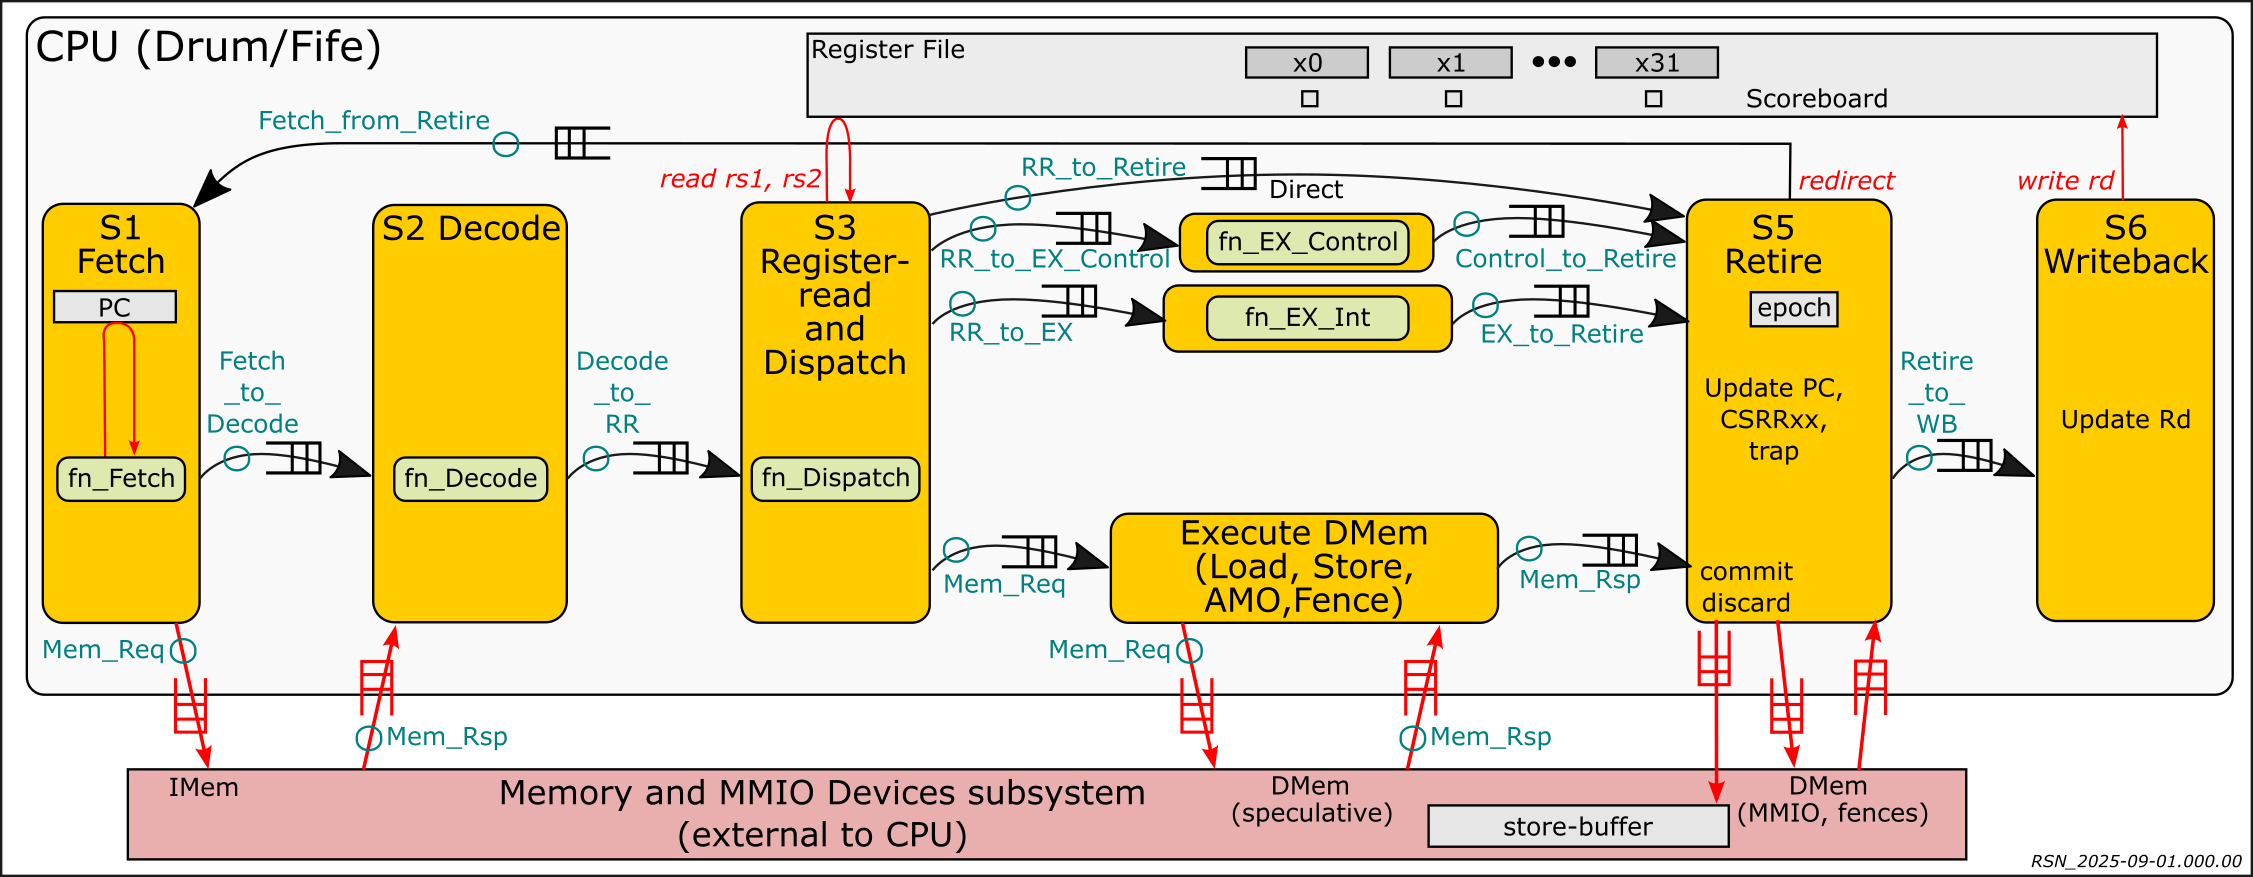
\includegraphics[width=\textwidth]
                  {Figures/RSN_2025-09-01.000.00_FifeDrum_Stages_Multilayer_L1_L2_L3}
 \end{minipage}
 \hfill
 \begin{minipage}{0.49\textwidth}\scriptsize
  The {\FIFE} pipeline raises four new concerns:
  \begin{itemize}

    \item
      ``In-order retirement'': the Execute pipelines (Stage 4, or S4) may
      operate at different speeds (number of clock cycles), so the
      order in which their results arrive at S5 may be different from
      the order in which they entered S4 from S3.  But instructions
      must (logically) be performed in order.

    \vspace*{1ex}

    \item PC prediction to keep the pipeline full, and recovery from misprediction.

    \vspace*{1ex}

    \item Managing register ``hazards'': correct ordering of reads and
       writes of GPRs for different instructions.

    \vspace*{1ex}

    \item Speculative memory STOREs:
       {\tt EX\_DMem} may execute a LOAD/STORE instruction $I_n$ before we
       have completed instruction $I_{n-k}$ that is logically ahead of
       it (in one of the other S4 pipelines).  If $I_{n-k}$ is
       discarded (misprediction, trap, interrupt), we should discard
       $I_n$, {\ie} its STORE side-effect should not be performed.

  \end{itemize}
  We describe the solutions in the next few slides.
 \end{minipage}

\end{center}

\end{frame}

% ================================================================

\begin{frame}[fragile]
\frametitle{The {\FIFE} pipeline: In-order retirement}

\begin{center}\scriptsize
 \begin{minipage}{0.6\textwidth}\scriptsize
  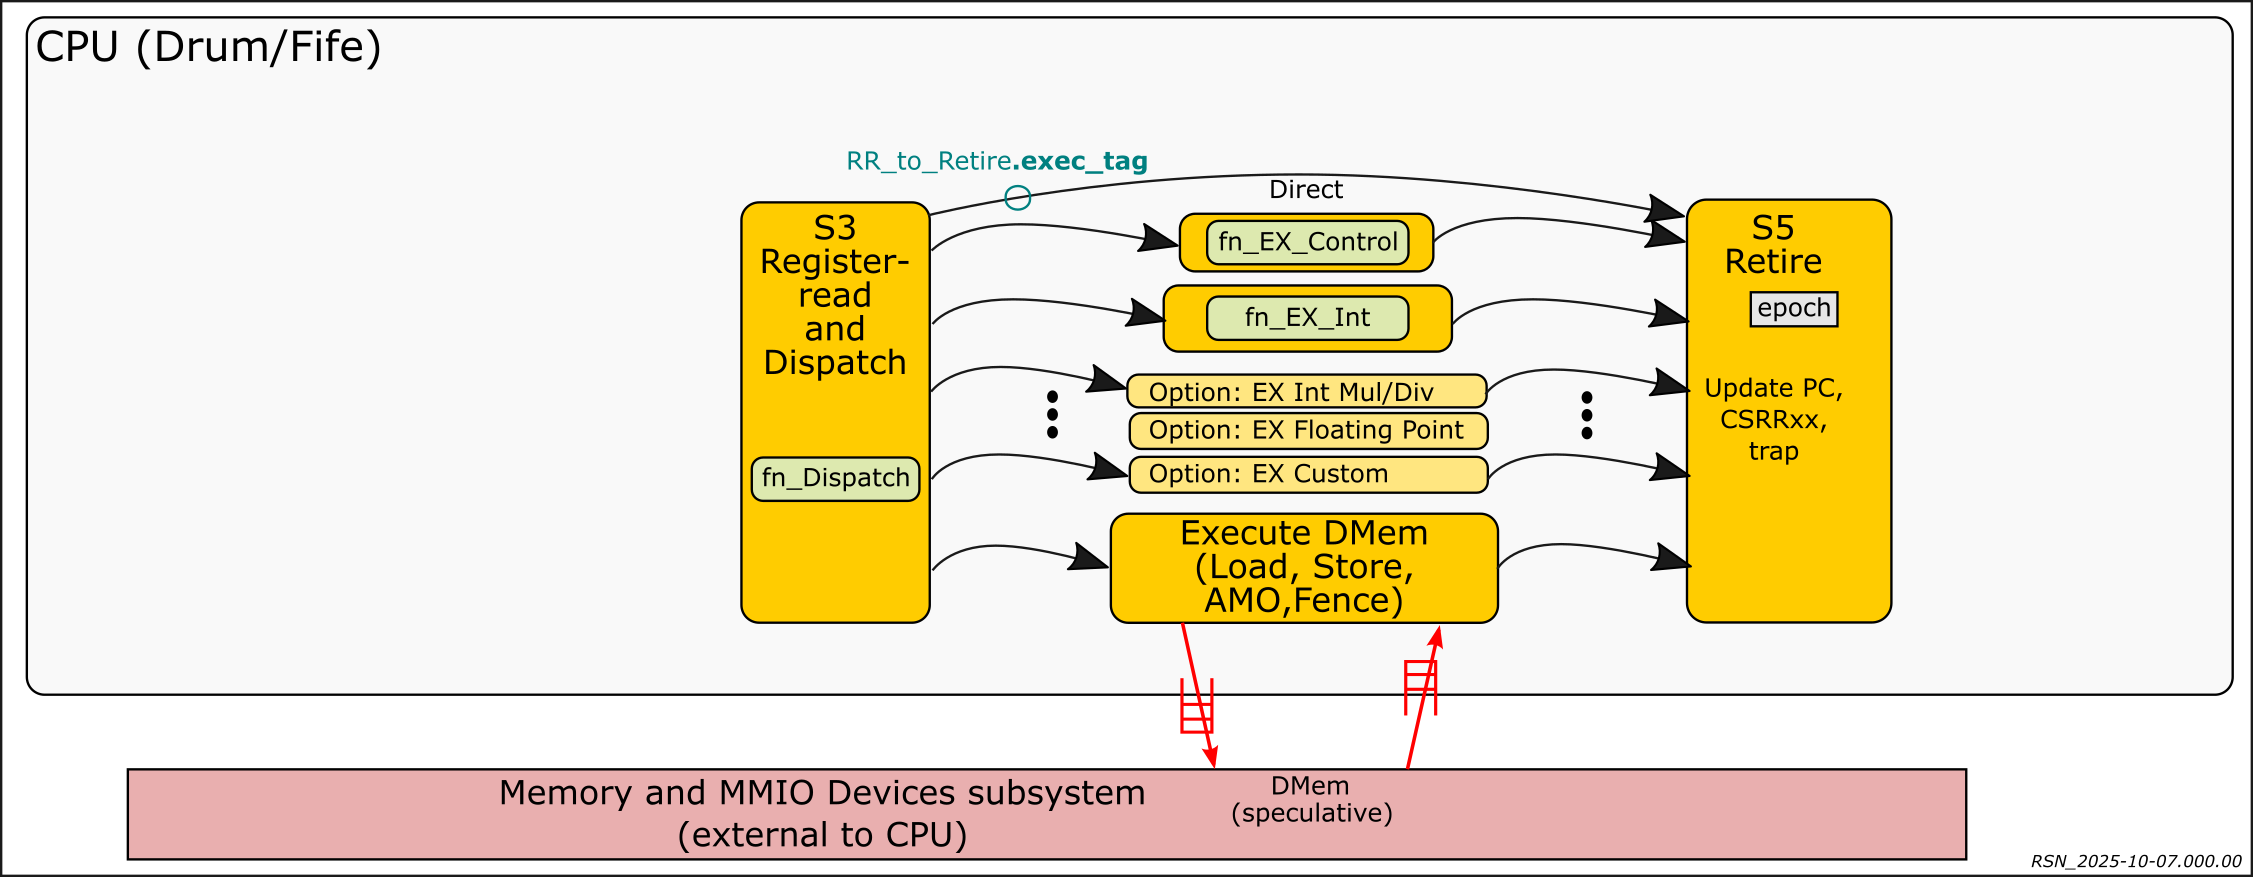
\includegraphics[width=\textwidth]
                  {Figures/RSN_2025-10-07.001.00_Concurrent_Exec_Pipes.png}
 \end{minipage}
 \hm
 \begin{minipage}{0.37\textwidth}\scriptsize

  The Execute pipelines (Stage 4, or S4) may operate at different
  speeds (number of clock cycles), so the order in which their results
  arrive at S5 may be different from the order in which they entered
  S4 from S3.  But instructions must (logically) be performed in
  order.

  \vspace*{1ex}

  Note that each of the S4 paths is FIFO-like (in order) even though
  their transit latencies may vary.

  \vspace*{5ex}

  Solution:
  \begin{itemize}
    \item In Stage 3 (S3), for \emph{every} instruction, we
      communicate a struct on the ``Direct'' path.

      \vspace*{1ex}

      We optionally \emph{also} communicate a struct on one of the
      other paths (INT, Control, DMem) if it is that kind of
      instruction.

    \item In Stage 5 (S5), we use the struct at the head of the Direct
      path to decide whether or not to consume a struct from one of
      the other paths (INT, Control, DMem), and we retire the
      instruction.
  \end{itemize}
 \end{minipage}
\end{center}

\end{frame}

% ================================================================

\begin{frame}[fragile]
\frametitle{The {\FIFE} pipeline: PC prediction and recovery from misprediction}

\begin{center}\scriptsize
 \begin{minipage}[t]{0.48\textwidth}\scriptsize
  In Stage 1 (S1) (``Fetch''), when we issue a memory request for an
  instruction, the \emph{only} information we have about it is the PC.

  \vspace*{1ex}

  What PC should we use to fetch the next instruction, in order to
  keep the pipeline full?  Normally the next PC is PC+4, but not if
  the fetched instruction turns out to be a (taken)
  BRANCH/JAL/JALR/ECALL/EBREAK, or if the instruction traps (memory
  fault on Fetch or LOAD/STORE, illegal instruction, misaligned
  BRANCH/JAL/JALR target), or if we take an interrupt, {\etc} These
  outcomes are only known in later stages.

  \vspace*{1ex}

  When we finally know that an instruction's successor was
  mispredicted, how do we recover?

 \end{minipage}
 \hm
 \begin{minipage}[t]{0.48\textwidth}\scriptsize
  \begin{itemize}

    \item In S1, we \emph{predict} (guess) the next PC so we can do
      the next fetch. In {\FIFE} we blindly predict PC+4.  \emph{Much}
      better prediction is possible by analyzing the history of PCs;
      this is left for your future study.

    \vspace*{0.5ex}

    \item In Stage 5 (S5), we maintain an ``epoch'' register.  When we
      know there was a misprediction, we increment the epoch, and send
      a struct to S1 indicating the correct PC and new epoch.

    \vspace*{0.5ex}

    \item S1 starts fetching from the correct PC. For each
      instruction, its epoch accompanies it through the pipeline.

      In S5, we discard all instructions of the wrong epoch, and start
      retiring again when we see the correct epoch.

  \end{itemize}
 \end{minipage}

 \vspace*{1ex}

 \begin{minipage}{0.6\textwidth}\scriptsize
  
\includegraphics[width=\textwidth]{Figures/RSN_2025-09-15.000.00_Fife_Epochs.png}
 \end{minipage}

\end{center}

\end{frame}

% ================================================================

\begin{frame}[fragile]
\frametitle{The {\FIFE} pipeline: Managing register ``hazards''}

\begin{center}\scriptsize
 \begin{minipage}[t]{0.48\textwidth}\scriptsize

  Suppose an instruction $I_n$ is in S4 or S5, and will write a result
  to GPR[x7].

  \vspace*{1ex}

  Suppose a later instruction (say, $I_{n+1}$) tries to
  read from GPR[x7]. To avoid reading a stale value, it needs to wait
  (``stall'') until $I_n$ has updated GPR[x7].  The danger of
  accessing the wrong GPR[$j$] value is called a ``hazard''.
 \end{minipage}
 \hm
 \begin{minipage}[t]{0.48\textwidth}\scriptsize
  \begin{itemize}

    \item Along with the GPRs, we maintain, for each GPR, a 1-bit
    ``busy'' value.  The collection of 32 bits is called a
    ``scoreboard''.

    \vspace*{0.5ex}

    \item When an instruction arrives at S3 we wait (stall), if
     necessary, until its registers are not busy.  Then, we can read
     its Rs1 and Rs2 registers.  If it has a destination register Rd,
     we mark it busy before allowing the instruction to move on to S4.

    \vspace*{0.5ex}

    \item In S5, when we retire an instruction, if it has an Rd, we
     send a struct back to S3 to free its busy bit (thereby possibly
     releasing an instruction might have been stalled waiting for this.

  \end{itemize}
 \end{minipage}

 \vspace*{2ex}

 \begin{minipage}{0.6\textwidth}\scriptsize
  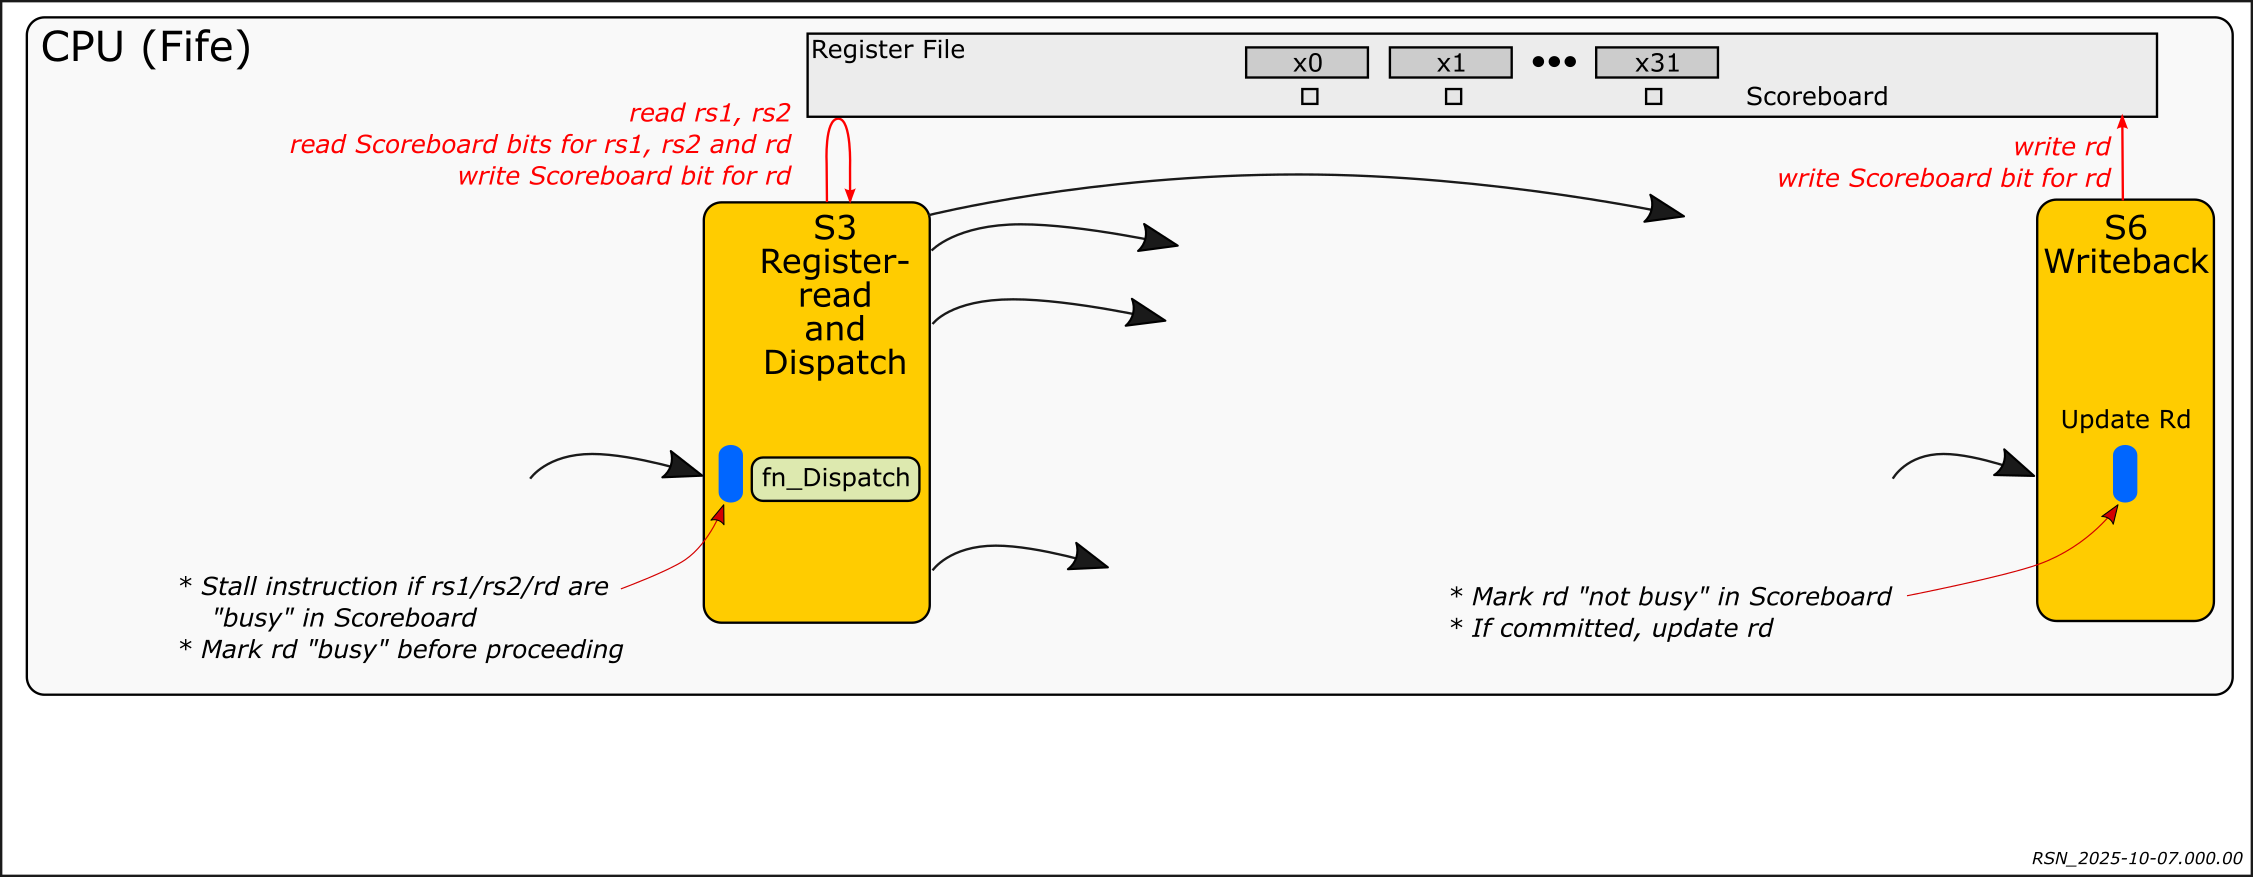
\includegraphics[width=\textwidth]{Figures/RSN_2025-10-07.000.00_Scoreboard.png}
 \end{minipage}

\end{center}

\end{frame}

% ================================================================

\begin{frame}[fragile]
\frametitle{The {\FIFE} pipeline: Speculative memory LOADs and STOREs}

\begin{center}\scriptsize
 \begin{minipage}[t]{0.62\textwidth}\scriptsize

    {\tt EX\_DMem} may execute a LOAD/STORE instruction $I_n$ before
    we have completed instruction $I_{n-k}$ that is logically ahead of
    it (in one of the other S4 pipelines).  If $I_{n-k}$ is discarded
    (misprediction, trap, interrupt), we should discard $I_n$, {\ie}
    its STORE side-effect should not be performed.

    \vspace*{5ex}

    \begin{minipage}{\textwidth}\scriptsize
     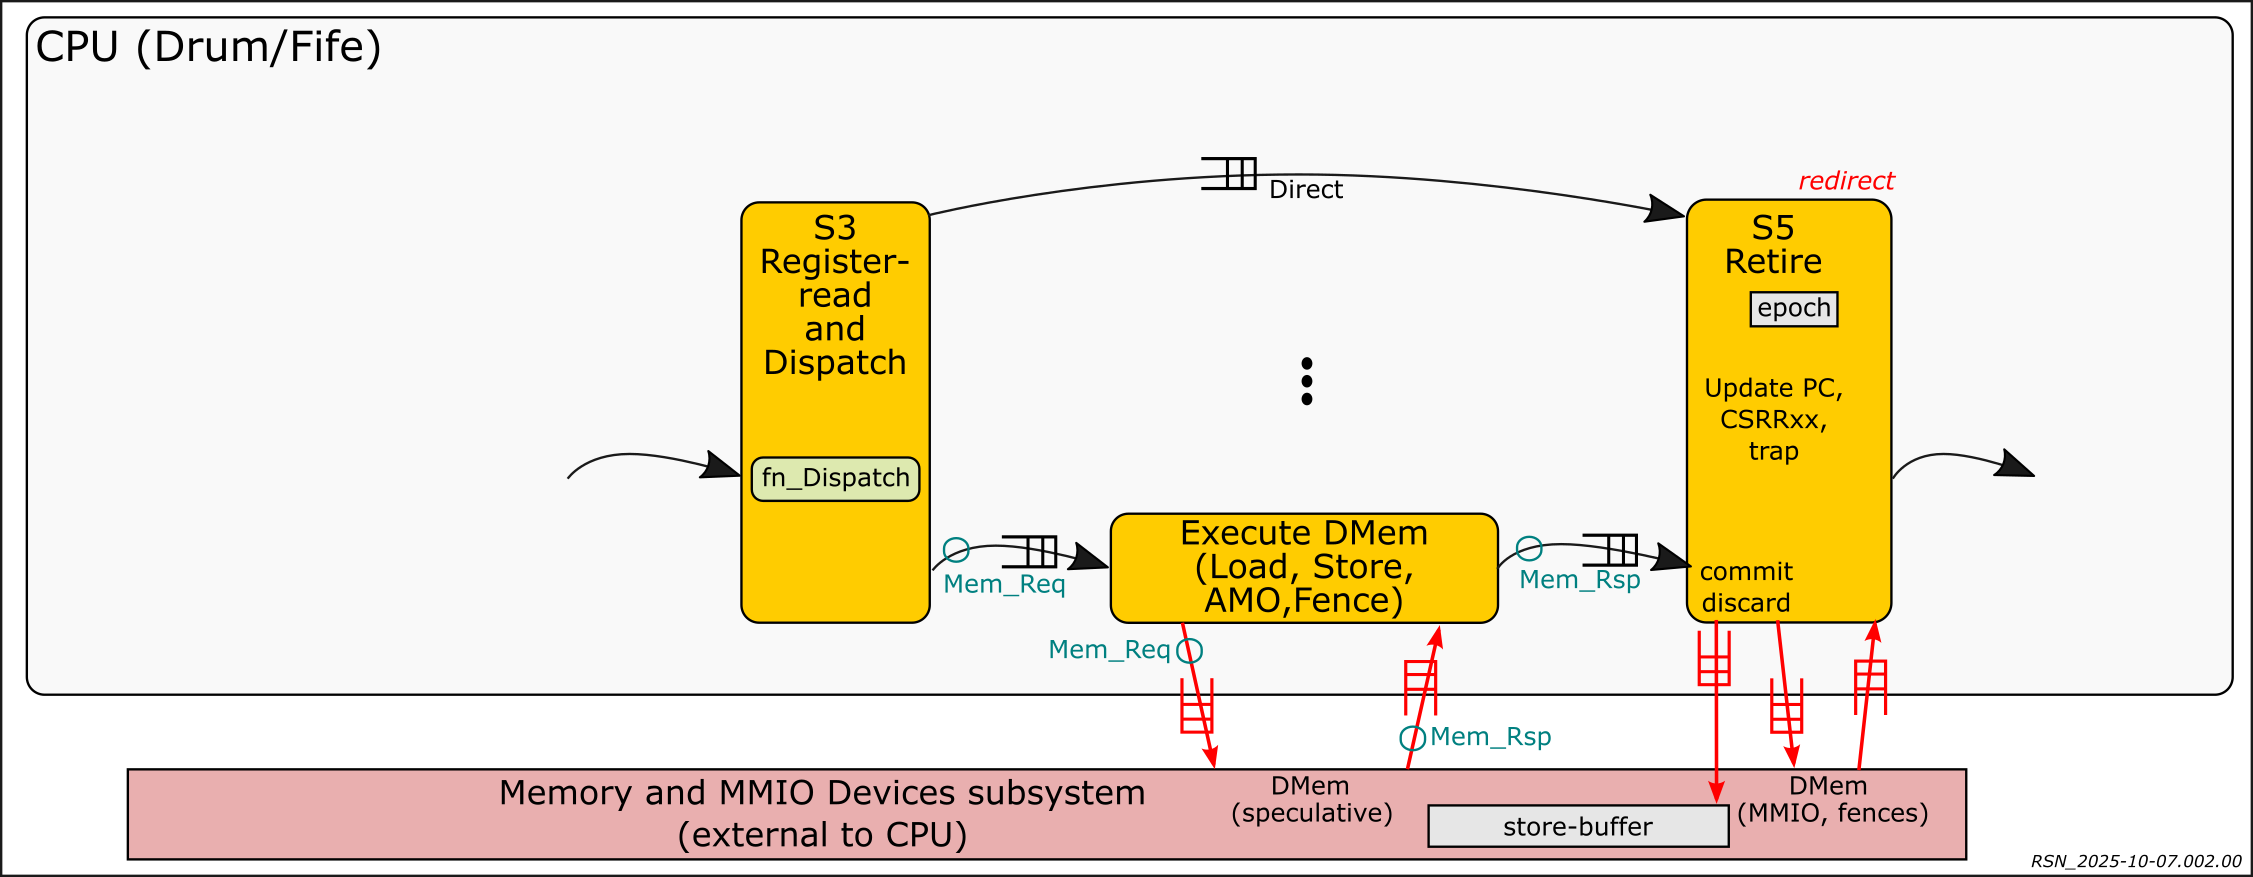
\includegraphics[width=\textwidth]{Figures/RSN_2025-10-07.002.00_Store_Buffer.png}
    \end{minipage}
 \end{minipage}
 \begin{minipage}[t]{0.37\textwidth}\scriptsize
  \begin{itemize}

    \item In the Memory System (outside the CPU) we maintain a ``Store
      Buffer'', where we keep an in-order record of any STORE memory
      updates.

    \vspace*{0.5ex}

    \item For a LOAD, we check the store buffer for the most recent
      update, if any, for the address of interest, and only do a usual
      memory access if there is no such record.

    \vspace*{0.5ex}

    \item In S5, when we retire this instruction, we send a
    ``Commit/Discard'' struct to the Store Buffer indicating how to
    dispose of its oldest entry: store it in memory, or discard.

    \item For MMIO addresses, even LOADs can have side-effects.  We
      punt: the DMem\_Speculative port does nothing but return the
      memory request with a DEFERRED indication, and we perform the
      operation in S5 once we know we're committing this instruction
      (using a small sequential FSM).

  \end{itemize}
 \end{minipage}

\end{center}

\end{frame}

% ================================================================

\begin{frame}[fragile]
\frametitle{(Repeating earlier diagram, for convenience)}

\begin{center}
 \begin{minipage}{0.8\textwidth}\scriptsize
  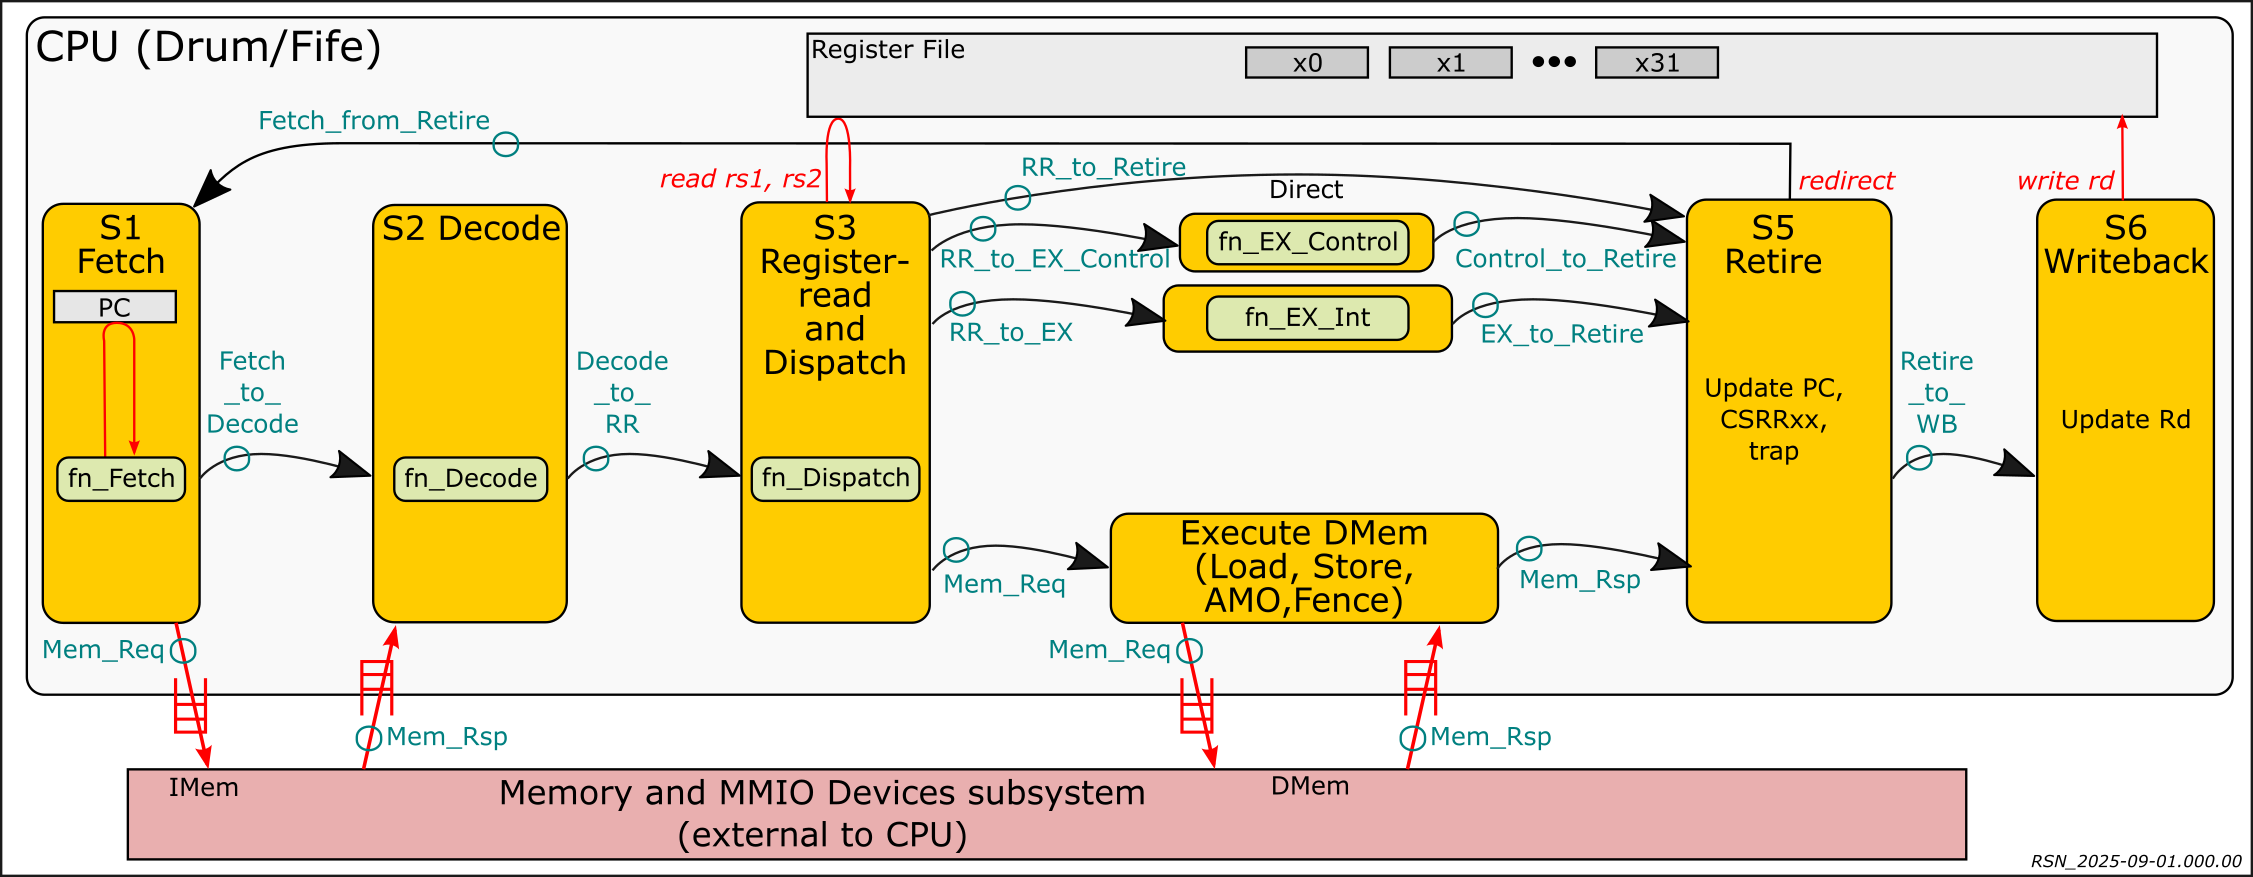
\includegraphics[width=\textwidth]
                  {Figures/RSN_2025-09-01.000.00_FifeDrum_Stages_Multilayer_L1_L3}
 \end{minipage}
\end{center}

\end{frame}

% ================================================================

\begin{frame}[fragile]
\frametitle{Let's read some code together: {\FIFE}'s S1 stage (fetch)}

\begin{center}\scriptsize
 \fbox{
  \begin{minipage}{0.9\textwidth}
   \begin{tabbing}
    Repository: \hmm \= {\BookRepo} \hmmmm \\
    Files:           \> {\tt Code/src\_Fife/S1\_Fetch.bsv} \\
    Focus on:        \> {\tt interface Fetch\_IFC}, {\tt module mkFetch}, {\tt rl\_Fetch\_req}
   \end{tabbing}
  \end{minipage}}

 \vspace*{5ex}
 
 \begin{minipage}{0.9\textwidth}
  \begin{itemize}

   \item In interface {\tt Fetch\_IFC} there are two outgoing FIFOs
     (to Decode and to Memory) and one incoming FIFO (PC redirection
     from S5).

   \item In module {\tt mkFetch} we instantite FIFOs for these interfaces.

   \item The rules {\tt rl\_Fetch\_req} and {\tt
     rl\_Fetch\_from\_Retire} are infinite loops (processes).  Each
     rule blocks (stalls/waits) until its rule-condition is true and
     all the implicit conditions of the methods it invokes are true;
     then it executes the rule body once; and this process repeats.

     For example, the implicit condition of a FIFO {\tt .enq} method
     is true only when there is space available in the FIFO (not
     full).  The implicit condition of IFO {\tt .first} and {\tt .deq}
     methods are true only when there is data available in the FIFO
     (non-empty).

   \item Rule {\tt rl\_Fetch\_req} uses the current PC to invoke
     function {\tt fn\_Fetch()}, and enqueues its two results into the
     two outgoing FIFOs.  It predictst the next PC as PC+4 (this line
     can be replaced to use a more sophisticated predictor that knows
     about the history of past PCs).

   \item Rule {\tt rl\_Fetch\_from\_Retire} handles redirections
     (struct that was sent from S5). It updates the PC and the epoch
     registers, affecting future fetches by rule {\tt rl\_Fetch\_req}.

  \end{itemize}
 \end{minipage}
\end{center}

\end{frame}

% ================================================================

\begin{frame}[fragile]
\frametitle{(Repeating earlier diagram, for convenience)}

\begin{center}
 \begin{minipage}{0.8\textwidth}\scriptsize
  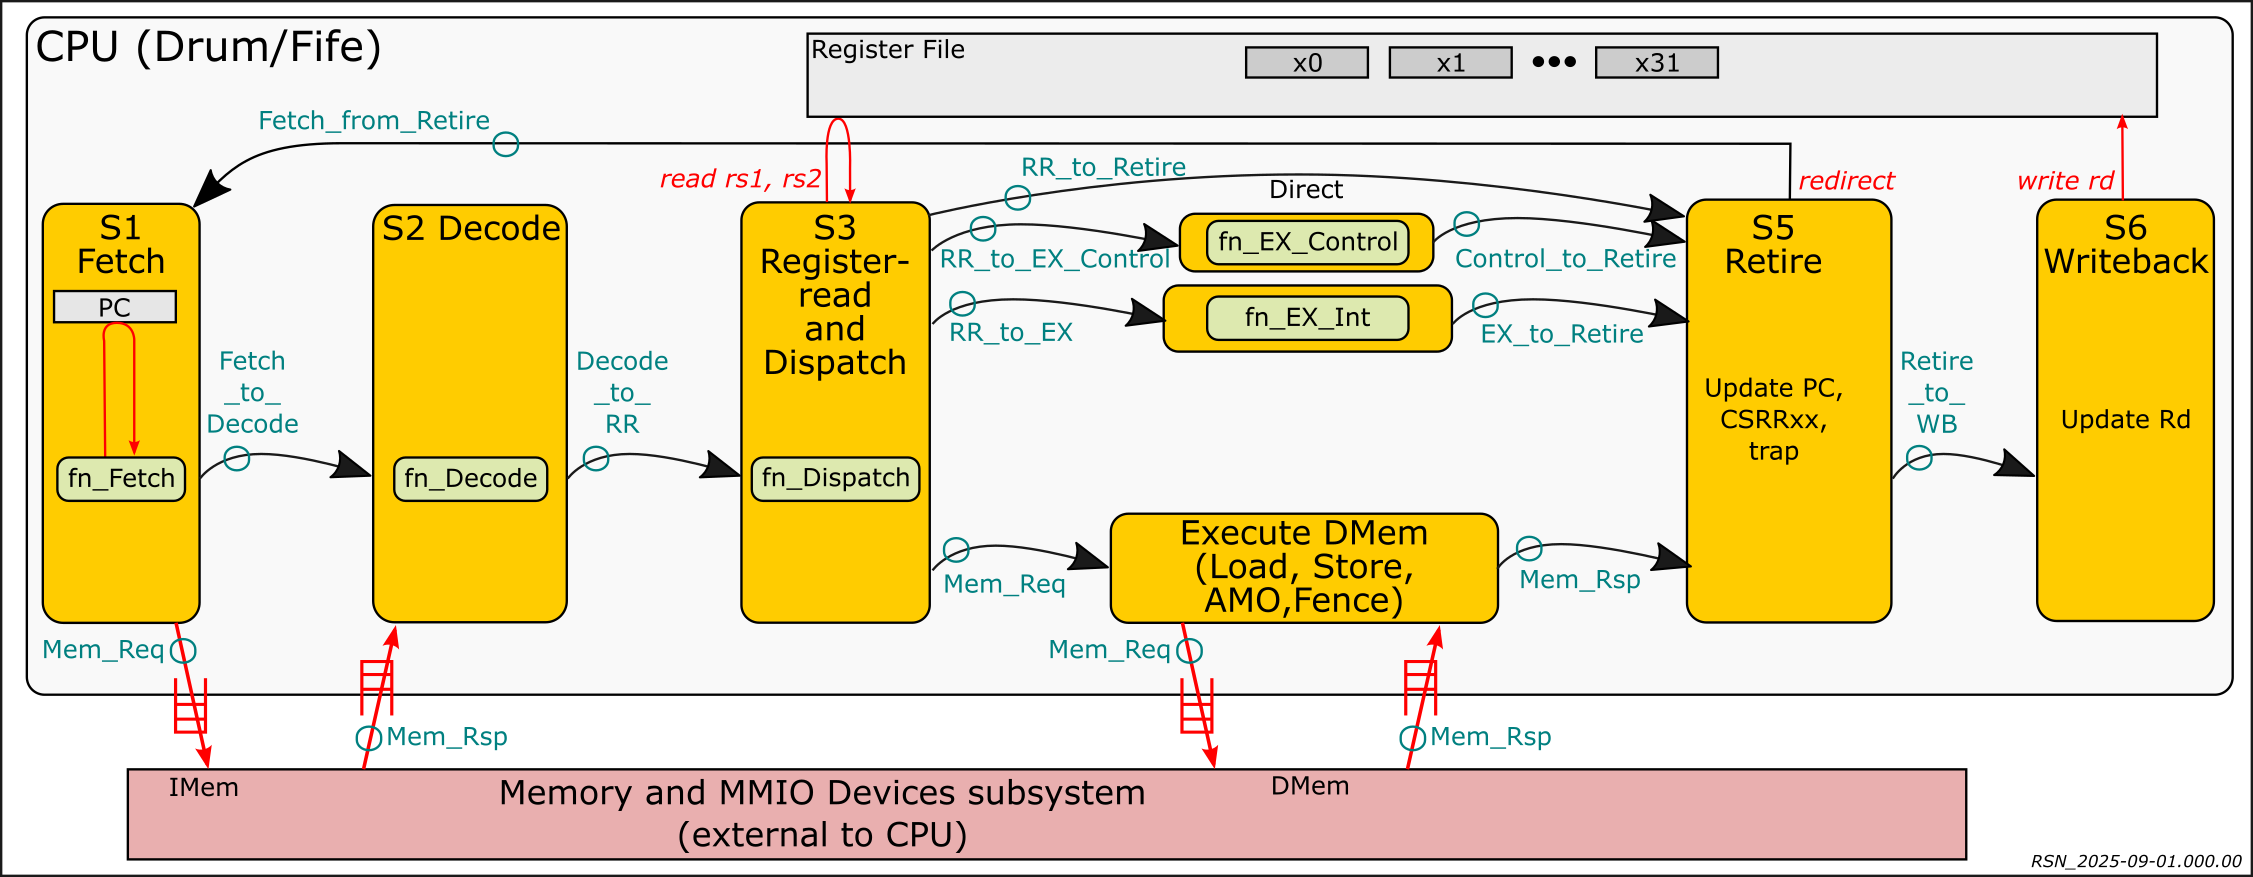
\includegraphics[width=\textwidth]
                  {Figures/RSN_2025-09-01.000.00_FifeDrum_Stages_Multilayer_L1_L3}
 \end{minipage}
\end{center}

\end{frame}

% ================================================================

\begin{frame}[fragile]
\frametitle{Let's read some code together: {\FIFE}'s S3 and S6 stages (register read and dispatch, and register writeback)}

\begin{center}\scriptsize
 \fbox{
  \begin{minipage}{0.9\textwidth}
   \begin{tabbing}
    Repository: \hmm \= {\BookRepo} \hmmmm \\
    Files:           \> {\tt Code/src\_Fife/S3\_RR\_S6\_WB.bsv} \\
    Focus on:        \> {\tt interface RR\_WB\_IFC}, {\tt module mkRR\_WB}
   \end{tabbing}
  \end{minipage}}

 \vspace*{5ex}
 
 \begin{minipage}{0.9\textwidth}
  \begin{itemize}

   \item In interface {\tt RR\_WB\_IFC} there is one input FIFO (from
     Decode), one output FIFO for each of the paths through S4, and
     one input FIFO for register and scoreboard updates from S5.

   \item In module {\tt mkFetch} we instantite FIFOs for these interfaces.

   \item The rule {\tt rl\_RR\_Dispatch} (stage S3) checks the
     scoreboard if the instruction's Rs1, Rs2 or Rd (if it has such
     register fields) are busy.

     In the if-then-else that follows, if the scoreboard indicates we
     must stall, then we do nothing.  This rule will try again, on the
     next clock

     If the scoreboard permits us to proceed, we read the rs1 and rs2
     registers and invoke {\tt fn\_Dispatch()} to produce the structs
     to be sent to the next stage.

     Note that we blindly read GPRs rs1 and rs2, whether or not the
     instruction has such fields.  There is no harm done if the
     instruction does not have such fields, since we only use them if
     relevant.  Avoiding an unnecessary conditional will save us a MUX
     (multiplexor), which can be an expensive in hardware.

   \item Rule {\tt rl\_WB\_from\_Retire} (stage S6) accepts a struct
     sent by S5 and updates the scoreboard to ``unbusy'' a register
     (whether the S5-retired instruction was speculative or not), and
     updates the register if it was not speculative.

  \end{itemize}
 \end{minipage}
\end{center}

\end{frame}

% ================================================================

\begin{frame}[fragile]
\frametitle{{\FIFE}'s speculative LOADs and STOREs}

\begin{center}\scriptsize
 \begin{minipage}{0.9\textwidth}
  \begin{itemize}

   \item These are handled by the ``Store\_Buffer'' in the memory
     system, which is outside the CPU.

   \vspace*{2ex}

   \item Being outside the CPU, and therefore not our focus today, we
     do not discuss this further here.  In fact, we handle it in
     imported C code. If interested, please see the files: \\
     \hm {\tt Code/src\_Top/Mems\_Devices.bsv} \\
     \hm {\tt Code/src\_Top/C\_Mems\_Devices.c}
  \end{itemize}
 \end{minipage}
\end{center}

\end{frame}

% ================================================================

\begin{frame}[fragile]
\frametitle{(Repeating earlier diagram, for convenience)}

\begin{center}
 \begin{minipage}{0.8\textwidth}\scriptsize
  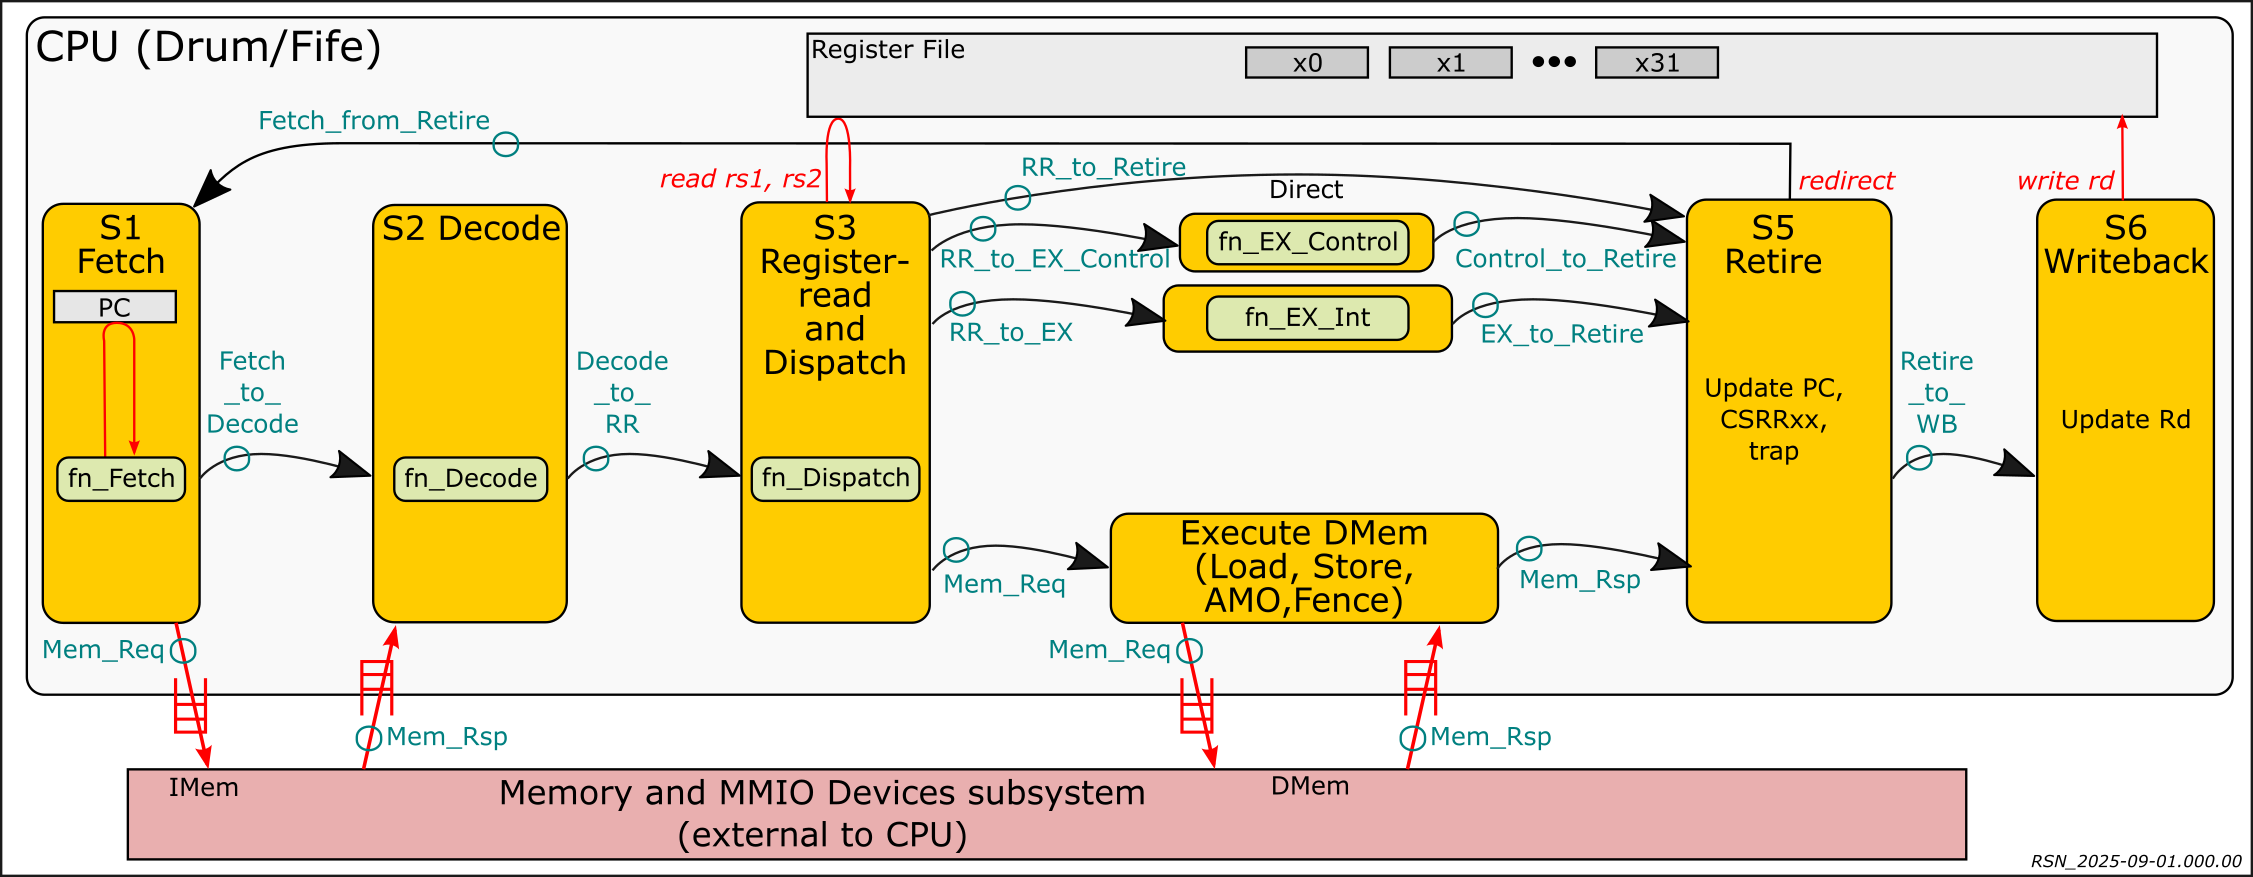
\includegraphics[width=\textwidth]
                  {Figures/RSN_2025-09-01.000.00_FifeDrum_Stages_Multilayer_L1_L3}
 \end{minipage}
\end{center}

\end{frame}

% ================================================================

\begin{frame}[fragile]
\frametitle{Let's read some code together: Interface for {\FIFE}'s S5 stage (retire/commit)}

\begin{center}\scriptsize
 \fbox{
  \begin{minipage}{0.9\textwidth}
   \begin{tabbing}
    Repository: \hmm \= {\BookRepo} \hmmmm \\
    Files:           \> {\tt Code/src\_Fife/S5\_Retire.bsv} \\
    Focus on:        \> interface {\tt Retire\_IFC}
   \end{tabbing}
  \end{minipage}}

 \vspace*{5ex}
 
 \begin{minipage}{0.9\textwidth}
  \begin{itemize}

   \item The interface {\tt Retire\_IFC} contains:
     \begin{itemize}\scriptsize
       \item An input FIFO from S3: {\tt fi\_RR\_to\_Retire}
       \item Input FIFOs from S4: {\tt fi\_EX\_Control\_to\_Retire},
             {\tt fi\_EX\_Int\_to\_Retire} and
	     {\tt fi\_DMem\_S\_rsp} (speculative DMem response)
       \item An output FIFO {\tt fo\_DMem\_S\_commit} (speculative DMEM commit/discard)
       \item An output FIFO {\tt fo\_DMem\_req} and input FIFO {\tt fi\_DMem\_rsp}
           for MMIO (non-speculative) memory accesses
       \item An output FIFO {\tt fo\_Fetch\_from\_Retire} to S1 for PC redirections

       \item An output FIFO {\tt fo\_WB\_from\_Retire} to S3 for
             updating the GPRs and scoreboard.
     \end{itemize}

   \vspace*{5ex}

   \item The remaining sub-interfaces are for a timer and timer interrupt,
     and debugger control; we do not have time to discuss these today.

  \end{itemize}
 \end{minipage}
\end{center}

\end{frame}

% ================================================================

\begin{frame}[fragile]
\frametitle{Actions in module implementing {\FIFE}'s S5 stage}

 \begin{center}\scriptsize
  \begin{minipage}{0.6\textwidth}\scriptsize
   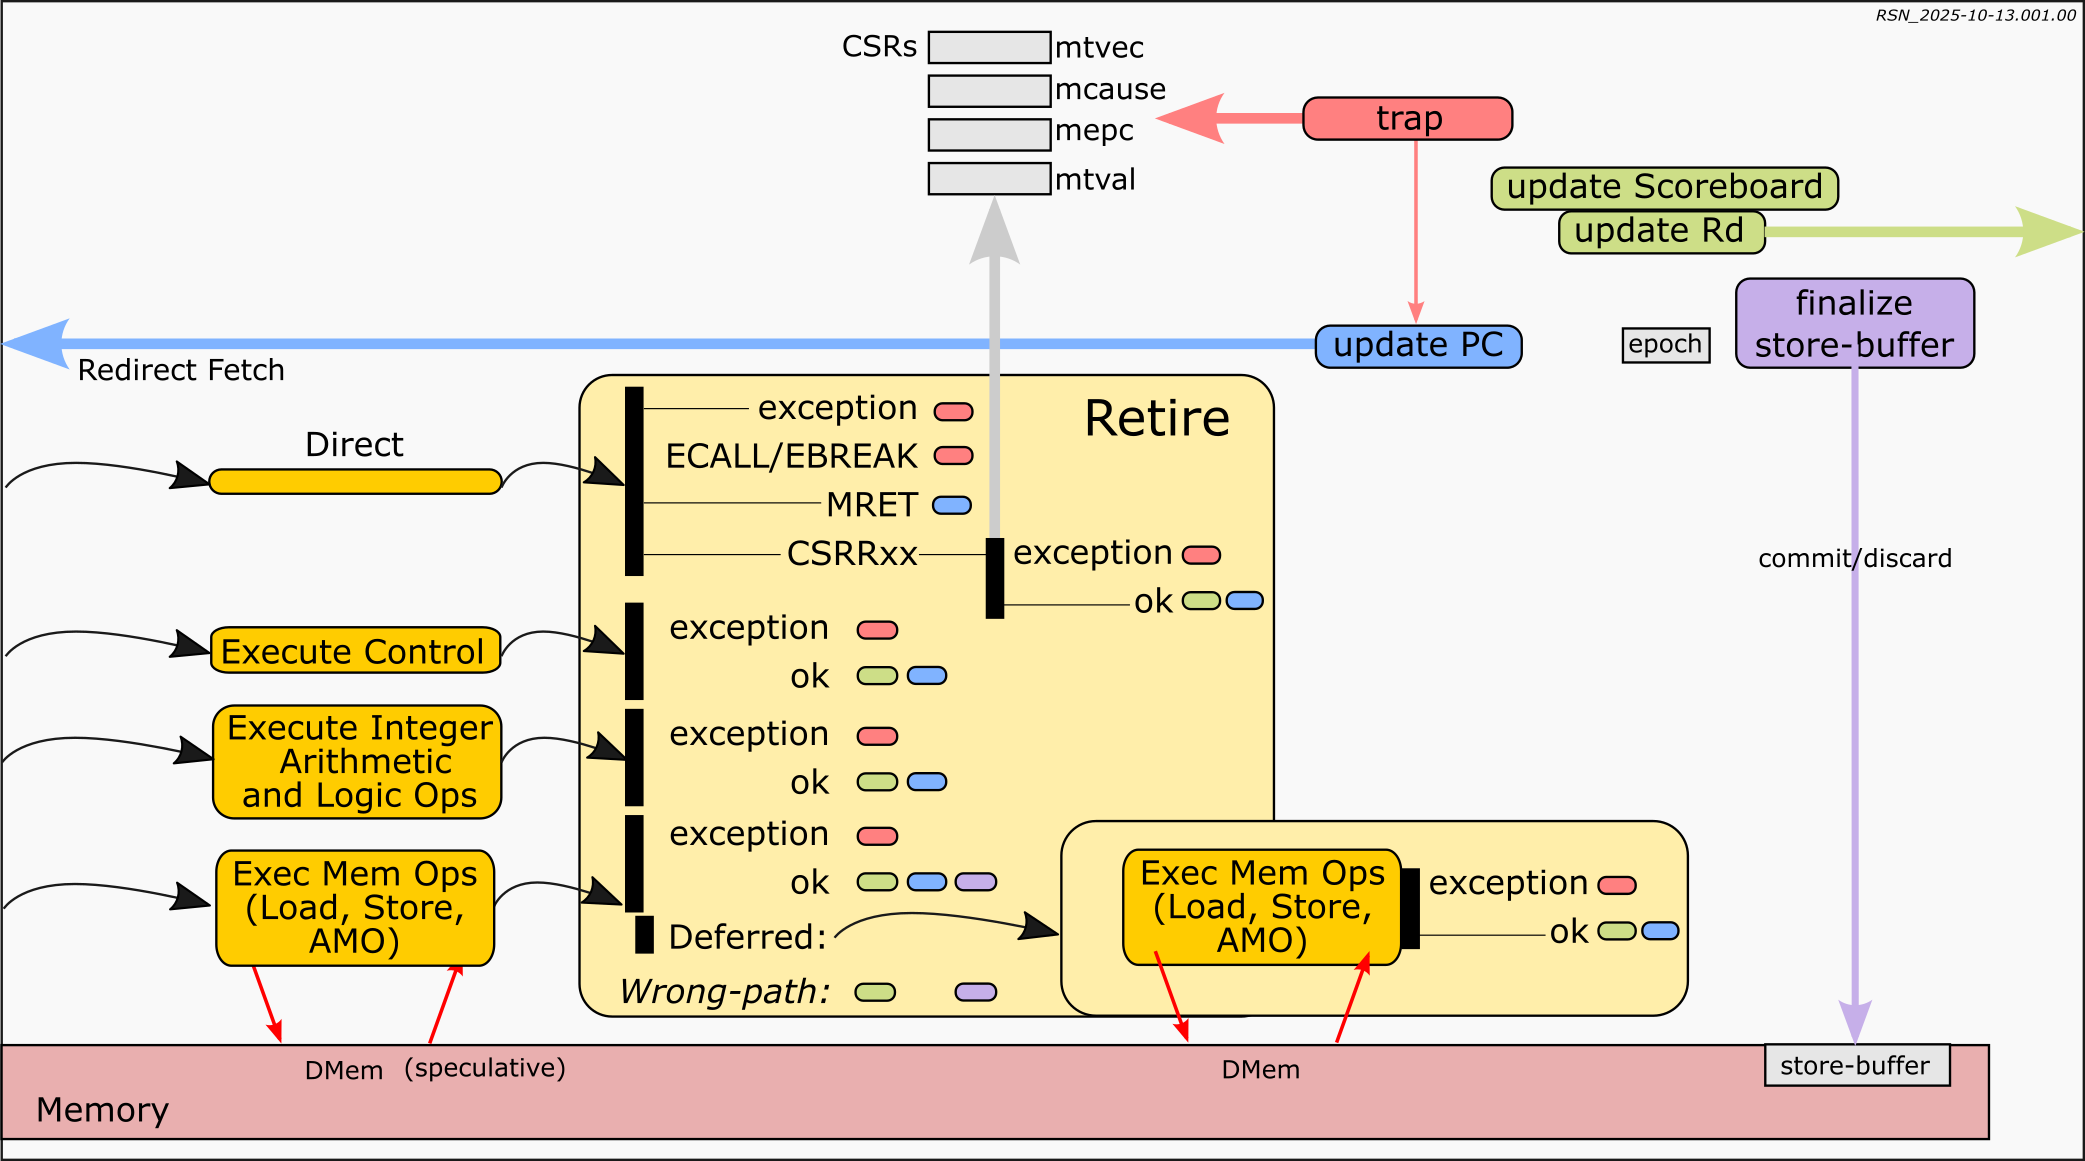
\includegraphics[width=\textwidth]{Figures/RSN_2025-10-13.001.00_Fife_Retire_L1_L2.png}
  \end{minipage}
  \begin{minipage}{0.38\textwidth}
   \begin{itemize}

    \item There are \emph{many} rules in the S5 {\tt mkRetire} module,
          each taking care of some particular situation on the four
          input FIFOs.

    \item The rule actions share many common actions, indicated by the
          colored lozenges in the diagram.

    \item The ``update PC'' action (blue) is only performed on a misprediction.

   \end{itemize}
   \begin{itemize}\tiny

    \item {\Eg} If the Direct path carries a CSRRxx instruction, we
          execute the CSR function. If that raises an exception, we do
          the trap action, else we update Rd/Scoreboard.

    \item {\Eg} If the Direct path carries a LOAD/STORE instruction,
          and the DMem response is DEFERRED (due to MMIO address), we
          now execute the memory ops. If this raises an exception, we
          do the trap action, else we update Rd/Scoreboard.

    \item {\Eg} if the Direct path indicates a wrong-path instruction
          (wrong epoch), if necessary we pop one of the other three incoming FIFOs;
          if necessary we update the Scoreboard; if necessary we finalize the
          store-buffer by sending it a ``Discard'' message.

   \end{itemize}
  \end{minipage}

 \end{center}
\end{frame}

% ================================================================

\begin{frame}[fragile]
\frametitle{Let's read some code together: Module implementing {\FIFE}'s S5 stage}

\begin{center}\scriptsize
 \fbox{
  \begin{minipage}{0.9\textwidth}
   \begin{tabbing}
    Repository: \hmm \= {\BookRepo} \hmmmm \\
    Files:           \> {\tt Code/src\_Fife/S5\_Retire.bsv} \\
    Focus on:        \> ... rules (see below) ...
   \end{tabbing}
  \end{minipage}}

 \vspace*{5ex}
 
 \begin{minipage}{0.9\textwidth}
  \begin{itemize}

    \item Function {\tt fa\_redirect\_Fetch} is a help-function
      invoked from numerous rules to create a redirection struct and
      send it to S1 (enqueue on the outgoing FIFO to S1).

    \item Similarly, function {\tt fa\_update\_rd} is a help-function
      invoked from numerous rules to create a GPR/scoreboard-update
      struct and send it to S3 (enqueue on the outgoing FIFO to S3).

    \item {\tt Bool wrong\_path} is the condition of whether the next
      incoming instrucion from S4 is to be discarded (wrong epoch) or
      committed.

      Rule {\tt rl\_Retire\_wrong\_path} performs the action of
      discarding wrong-path instructions including, if necessary,
      releasing any busy register in the scoreboard (message to S3)
      and discarding any pending STORE in the Store Buffer.

    \item Rule {\tt rl\_Retire\_Direct\_exception} retires any
      exception that was discovered in stages S2-S3 (including fetch
      memory-access errors and illegal instructions).

    \item Rules {\tt rl\_Retire\_EX\_Control} and {\tt
      rl\_Retire\_EX\_Int} retire BRANCH, JAL, JALR and integer ALU
      instructions that came through the {\tt EX\_Control} and {\tt
      EX\_Int} S4 paths.

    \item Rule {\tt rl\_Retire\_EX\_DMem} commits LOAD/STORE
      instructions that were performed speculatively ({\ie} not
      DEFERRED).

    \item Rule {\tt rl\_Retire\_DMem\_deferred} handles DEFERRED
      memory instructions, now issuing the memory request.  Rule {\tt
      rl\_Retire\_DMem\_rsp} handles the response.

    \item In any of the preceding rules, if there was an exception
      (trap or interrupt), they set up rule {\tt rl\_exception} to
      handle it.

  \end{itemize}
 \end{minipage}
\end{center}

\end{frame}

% ================================================================

\begin{frame}[fragile]

\begin{center}
  {\LARGE Pause ...}

 \vspace*{8ex}

 \begin{minipage}{0.8\textwidth}

   ... and we're done reading {\FIFE} code!    \hmmmm {\LARGE \bf Congratulations!}

   \vspace*{2ex}

   {\scriptsize The key difference from a traditional programming
   language is the execution semantics based on \emph{concurrent
   rules}, a.k.a, \emph{Guarded Atomic Actions}, as opposed to
   traditional sequential statements.}

   \vspace*{10ex}

   This code can be compiled to Verilog which, in turn, can be built
   into a Verilog simulation executable, or taken through FPGA or ASIC
   flows into real hardware.

 \end{minipage}

 \vspace*{5ex}

 And that's next on the agenda ...

\end{center}

\end{frame}

% ****************************************************************
% ****************************************************************
% ****************************************************************

\section{{\FIFE}: Generating Verilog, Simulation}

\begin{frame}[fragile]

\frametitle{Contents}

\begin{center}
 \hmm
 \begin{minipage}{0.5\textwidth}
  \tableofcontents
 \end{minipage}
 \hmm
 \begin{minipage}{0.3\textwidth}\scriptsize\it
  \vstrut{0em}{20ex} \\
  \fbox{
   \begin{minipage}{\textwidth}\scriptsize\it
    {\bf {\FIFE}: Generating Verilog, Simulation}
    \begin{tabbing} % Verse
      It's important to take pause \\
      \hmm for instant gratification (some fun), \\
      So let's simulate often, \\
      \hmm it's just a compile-and-run; \\
      \\
      In BSV, like in Haskell \\
      \hmm and OCaml before, \\
      If it type-checks and compiles, \\
      \hmm it'll run, for almost sure. \\
      \\
      \\
      While Drum works correctly, \\
      \hmm Its execution is at best galumphing \\
      When we pipeline it (in Fife), \\
      \hmm We get its juices pumping.
    \end{tabbing}
   \end{minipage}}
 \end{minipage}
\end{center}

\end{frame}

% ================================================================

\begin{frame}[fragile]

\begin{center}

  \vstrut{0em}{10ex}

  {\LARGE {\FIFE}: Generating Verilog. Simulation.}

  \vspace*{10ex}\scriptsize

  \begin{minipage}{0.8\textwidth}

    Please refer back to Section~\ref{sec_Drum_simulation}
    (page~\pageref{sec_Drum_simulation})
    for the
    steps to build and run a {\DRUM} simulation.

    \vspace*{2ex}

    The steps for {\FIFE} simulation are exactly the same, just
    substitute ``Fife'' wherever you see ``Drum'' in the previous instructions.

  \end{minipage}

\end{center}

\end{frame}

% ****************************************************************
% ****************************************************************
% ****************************************************************

\section{CPU Verification}

\label{sec_verif_w_test_programs}

\begin{frame}[fragile]

\frametitle{Contents}

\begin{center}
 \hmm
 \begin{minipage}{0.5\textwidth}
  \tableofcontents
 \end{minipage}
 \hmm
 \begin{minipage}{0.3\textwidth}\scriptsize\it
  \vstrut{0em}{20ex} \\
  \fbox{
   \begin{minipage}{\textwidth}\scriptsize\it
    {\bf CPU Verification}
    \begin{tabbing} % Verse
      And now comes the part that does \\
      \hmm HW designers and managers terrify \\
      We can't be sure it's right \\
      \hmm Until our designs we verify.
    \end{tabbing}
   \end{minipage}}
 \end{minipage}
\end{center}

\end{frame}

% ================================================================

\begin{frame}[fragile]
\frametitle{Complexity of CPU verification}

\begin{center}\scriptsize
 Verifying a CPU is often much harder than verifying single-purpose hardware IP:

 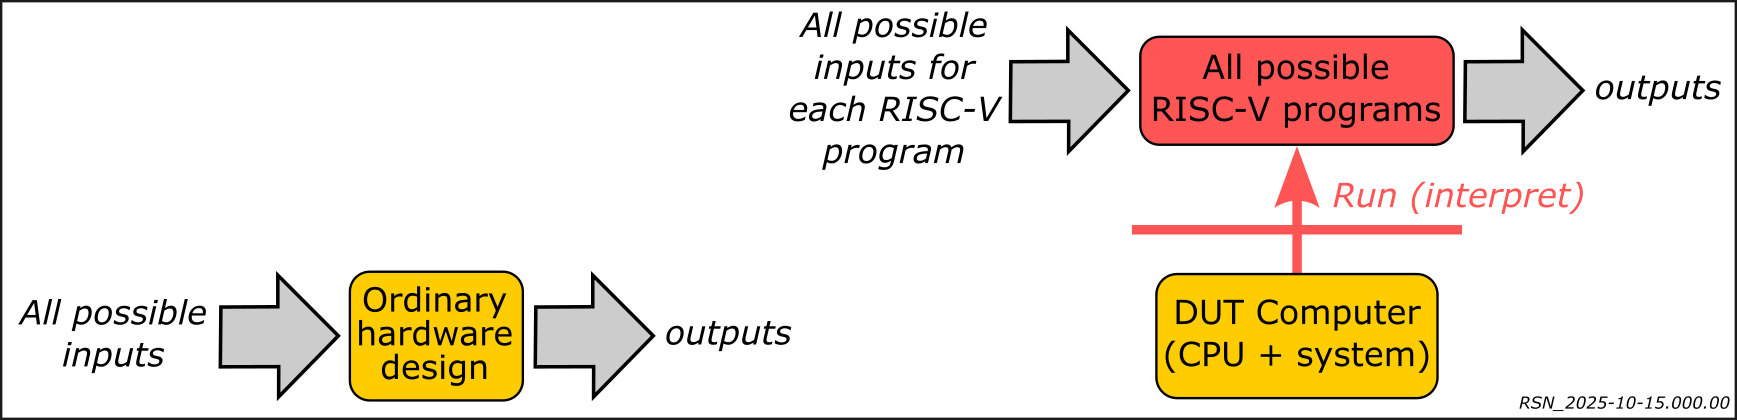
\includegraphics[width=0.8\textwidth]{Figures/RSN_2025-10-15.000.00_CPU_Verif_Complexity}

 \vspace*{5ex}

 \begin{minipage}{0.5\textwidth}\scriptsize
    ... because of the extra layer of interpretation ...

    \vspace*{2ex}

    Verifying an individual hardware IP may be hard because the space of
    \begin{itemize}
      \item all possible inputs
    \end{itemize}
    may be very large (infeasible to test all inputs).

    \vspace*{2ex}

    A CPU almost always has a \emph{very} large space of inputs:
    \begin{itemize}
      \item all possible RISC-V programs;
      \item for each such program, all possible inputs for that program
    \end{itemize}

 \end{minipage}
\end{center}

\end{frame}

% ================================================================

\begin{frame}[fragile]
\frametitle{Traditional Verification Methodologies for CPUs}

\begin{center}\scriptsize
 
 \vspace*{5ex}

 \begin{minipage}{0.9\textwidth}\scriptsize

    Please see the book for Chapters 11 and 12 for a discussion on
    traditional hardware verification methodologies for CPUs.

    \vspace*{2ex}

    Some of the methodologies are just like verifying software:
    \begin{itemize}

      \item Insert ``printfs'' (``{\tt \$display}'', ``{\tt \$write}
            in {\BSV}) at strategic points in the source code.

            \vspace*{1ex}

            See also Sections 11.3.1 and 11.3.2 for {\BSV}'s {\tt
            FShow} and {\tt Fmt} facilities for automatic
            ``pretty-printing'' of enums, structs, unions, and vectors.

      \item Run (simulate) the design on many possible test inputs and
            capture the {\$display} outputs in a log file.

      \item Study/analyze the log to identify erroneous behavior.

      \item Diagnose, fix, rebuild, and repeat.
    \end{itemize}

    There are sophisticated packages available from many sources to
    automate test generation and analysis;, a famous one is called
    {\bf UVM}.

    \vspace*{4ex}

    {\bf Debugging with Waveforms}: {\BSV} simulations (in Bluesim or
    Verilog simulation) can also produce so-called {\VCD} files which
    record all bit transitions during the simulation.  These {\VCD}
    files can be viewed in any \emph{Waveform Viewer} which displays
    the waveforms for each signal in the hardware.

    \vspace*{8ex}

    {\tiny {\bf CAUTION:} In the software world, the term ``verification''
    often refers exclusively to so-called \emph{formal verification},
    where a formal tool such as a theorem prover is used to
    \emph{prove} correctness based on the semantics of the hardware
    design language, and not using simulation.}

    {\tiny In the hardware world, the term ``verfication'' has
    traditionally been used for what the software world calls
    ``testing'', {\ie} running simulations on a suite of test inputs.}
 \end{minipage}
\end{center}

\end{frame}

% ================================================================

\begin{frame}[fragile]
\frametitle{Symmetric Tandem Verification}

\begin{center}\scriptsize
 
 \begin{minipage}{0.47\textwidth}\scriptsize
    This is a common technique for verifying CPUs.
    \begin{itemize}
     \item Relies on availability of a ``trusted`` simulator for the ISA.

           Example trusted simulators for the RISC-V ISA:
	   \begin{itemize}\scriptsize

            \item The official RISC-V ISA Formal Specification,
                  written in the language {\SAIL}, which can be
                  compiled and executed as a simulation.

            \item Spike, QEMU (widely used simulators for RISC-V, written in C++)
	   \end{itemize}

     \item A single RISC-V binary is executed on both the trusted
           simulator and on the CPU design.  Both the simulator and
           CPU design report the ``outcomes'' of each instruction
           (they both have to be instrumented to provide these
           outputs):

	   \begin{itemize}\scriptsize
            \item Register updates, if any (GPRs, FPRs, CSRs)
	    \item Memory updates, if any
	    \item Next PC
	    \item ...
	   \end{itemize}

     \item On an instruction-by-instruction basis, we compare the
            outcomes from the trusted simulator and the CPU design.
            Any discrepancy is likely a bug in the CPU design.

            (Comparison is automated, of course, to be able to cover
            millions of instructions.)

    \end{itemize}
 \end{minipage}
 \hm
 \begin{minipage}{0.5\textwidth}
  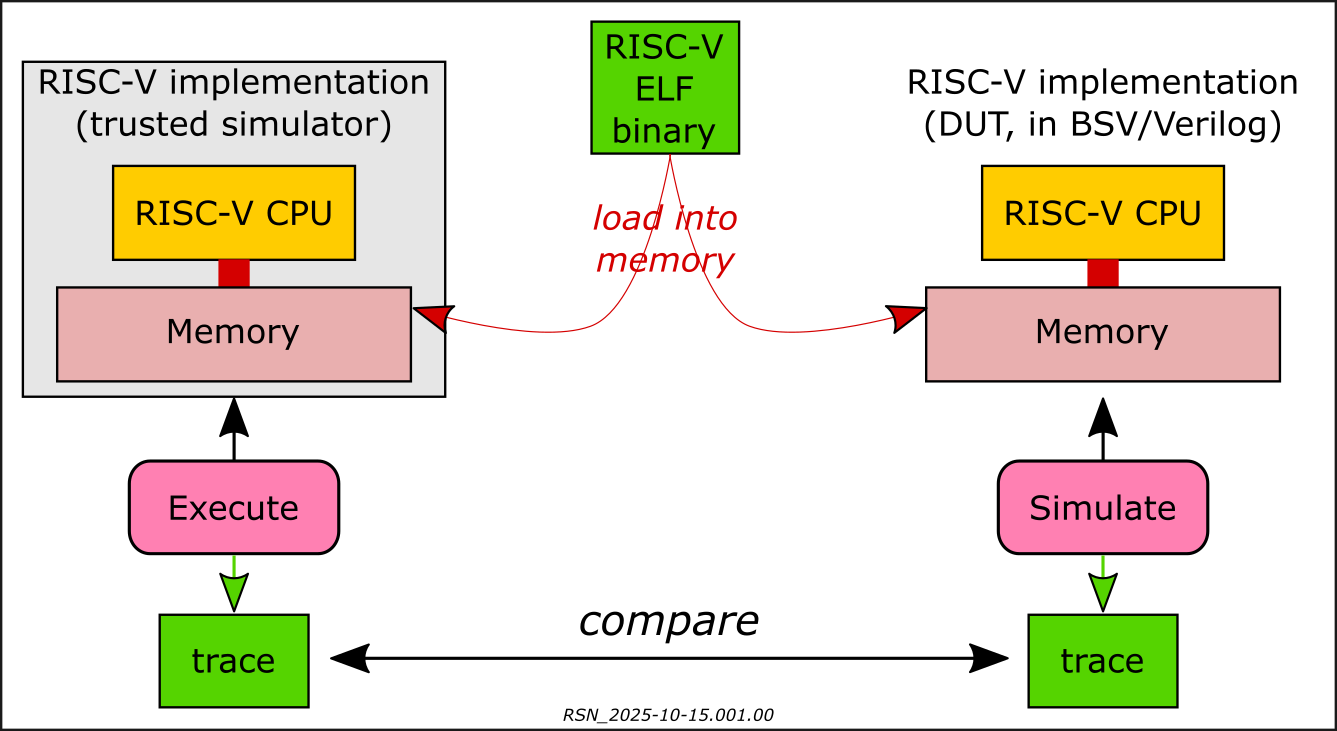
\includegraphics[width=\textwidth]
                  {Figures/RSN_2025-10-15.001.00_Symmetric_Tandem_Verification.png}

  \vspace*{5ex}
  {\scriptsize
  (See book Section 12.6.4 for ``Asymmetric'' Tandem Verification,
   which can also accommodate non-deterministic execution due to
   interrupts and MMIO reads.)}

 \end{minipage}
\end{center}

\end{frame}

% ****************************************************************
% ****************************************************************
% ****************************************************************

\section{Verification using {\TESTRIG}}

\label{sec_verif_w_TestRIG}

\begin{frame}[fragile]

\frametitle{Contents}

\begin{center}
 \hmm
 \begin{minipage}{0.5\textwidth}
  \tableofcontents
 \end{minipage}
 \hmm
 \begin{minipage}{0.3\textwidth}\scriptsize\it
  \vstrut{0em}{20ex} \\
  \fbox{
   \begin{minipage}{\textwidth}\scriptsize\it
    {\bf Verification using {\TESTRIG}}
    \begin{tabbing} % Verse
      Fear not, fellow designers \\
      \hmm Don't writhe in verification brig, \\
      From our friends at U.Cambridge, \\
      \hmm There's a lovely tool called TestRIG. \\
      \\
      Much simpler than hand-writing \\
      \hmm a few clever tests or formal assertions, \\
      It will generate a zillion tests, \\
      \hmm without requiring our exertions. \\
      \\
      By shrinking counterexamples automatically \\
      \hmm Debugging becomes much easier, \\
      We reach high assurance much sooner, \\
      \hmm Our stomachs much less queasier.
    \end{tabbing}
   \end{minipage}}
 \end{minipage}
\end{center}

\end{frame}

% ================================================================

\begin{frame}[fragile]
\frametitle{About {\TESTRIG}}

\begin{center}\scriptsize
 \begin{minipage}{0.4\textwidth}\scriptsize
  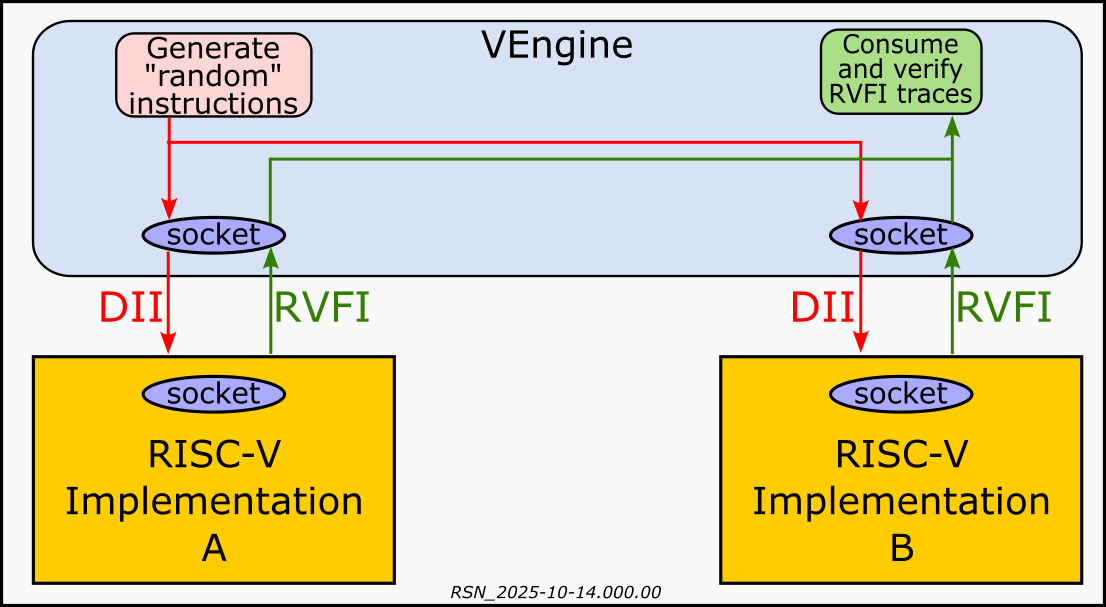
\includegraphics[width=\textwidth]{Figures/RSN_2025-10-14.000.00_TestRIG_Setup.png}
 \end{minipage}
 \hm
 \begin{minipage}{0.57\textwidth}\scriptsize
    {\TESTRIG} is a system for automated randomized testing of RISC-V implementations:

    \vspace*{1ex}

    \hm
    \begin{minipage}{0.9\textwidth}\tiny

     Joannou, A., Rugg, P., Woodruff, J., Fuchs, F.A., van der Maas, M.,
     Naylor, M., Roe, M., Watson,R.N.M, Neumann, P.G. and Moore, S.W.,
     \emph{Randomized testing of RISC-V CPUs using direct instruction injection},
     IEEE Design \& Test 41:1, February 2024, pp.40-49, DOI 10.1109/MDAT.2023.3262741
    \end{minipage}

    \vspace*{1ex}

    {\TESTRIG} is free and open-source software, available at: \\
    \hmm \url{https://github.com/CTSRD-CHERI/TestRIG}

    \vspace*{2ex}

    The VEngine generates randomized sequence of instructions.

    \vspace*{1ex}

    These instruction sequences are fed into two RISC-V
    implementations (A and B) using \emph{Direct Instruction
    Injection} (DII).  Typically,
    \begin{itemize}

     \item Implementation ``A'' is a RISC-V ``reference model''.  Here
           we use a simulator built from the official \emph{
           RISC-V Formal Specification} written in {\SAIL}
           (\url{https://github.com/riscv/sail-riscv}).

     \item Implementation ``B'' is the ``Design Under Test'' (or
           DUT). Here, it is a {\FIFE} or {\DRUM} simulation.
    \end{itemize}

    \vspace*{1ex}

    Both A and B report the outcomes of \emph{each} instruction to
    VEngine in the {\RVFI} format (``RISC-V Verification Interface'').
    The VEngine compares them and reports any discrepancy.

    \vspace*{1ex}

    Bonus: A failing instruction sequence could be hundreds/thousands
    of instructions long. The VEngine will automatically try to
    \emph{shrink} these sequences, often down to just a handful of
    instructions, making diagnosis of the error \emph{much} easier.

 \end{minipage}
\end{center}

\end{frame}

% ================================================================

\begin{frame}[fragile]
\frametitle{Fitting {\FIFE} (or any RISC-V CPU design) into {\TESTRIG}}

\begin{center}\scriptsize
 \begin{minipage}{0.5\textwidth}\scriptsize
  
\includegraphics[width=\textwidth]{Figures/RSN_2025-06-28.000.00_TestRIG_Fife.png}
 \end{minipage}
 \begin{minipage}{0.49\textwidth}\scriptsize
  \begin{itemize}

   \item {\tt mkCPU} is instrumented to collect the information for
         the {\tt RVFI\_DII\_Execution} struct.  These structs are
         streamed out on a new FIFO output interface {\tt
         fo\_rvfi\_reports} added to the {\tt CPU\_IFC} interface.

   \item We create a new module {\tt mkCPU\_and\_Mem} {\tiny (file {\tt
         TestRIG/src\_Top\_TestRIG/CPU\_and\_Mem.bsv})}.

         \vspace*{1ex}

         Unlike the normal {\tt Top.bsv} for standalone simulation,
         here {\bf we do not connect the IMem memory interfaces (for
         Fetch) to the memory model}.

         \vspace*{1ex}

         Instead, we have logic that, for every IMem request, consumes
         an instruction from {\TESTRIG} and feeds that in the IMem
         response (we ignore the instruction address (PC) in the
         request).

   \item {\tt mkRVFI\_Bridge\_Scalar} is from U.Cambridge GitHub: \\
         \hm \url{https://github.com/CTSRD-CHERI/BSV-RVFI-DII.git} \\
         We obtain a local copy (see {\tt TestRIG/vendor/}).

   \item We create a new top-level BSV module {\tt
         mkTop\_for\_TestRIG} {\tiny (file {\tt
         TestRIG/src\_Top\_TestRIG/Top\_TestRIG.bsv})} that
         instantiates {\tt mkRVFI\_Bridge\_Scalar} and {\tt
         mkCPU\_and\_Mem}, and connects up the reset, {\tt report} and
         {\tt getInst} interfaces.

  \end{itemize}
  \begin{center}
    And that's it! We're ready to roll!
  \end{center}
 \end{minipage}
\end{center}

\end{frame}

% ================================================================

\begin{frame}[fragile]
\frametitle{Let's read some code together: instrumenting the CPU for RVFI reports}

\begin{center}\scriptsize
 \fbox{
  \begin{minipage}{0.9\textwidth}
   \begin{tabbing}
    Repository: \hmm \= {\BookRepo} \hmmmm \\
    Files:           \> {\tt Code/vendor/RVFI\_DII\_Types/RVFI\_DII\_Types.bsv} \\
                     \> {\tt Code/src\_Common/RVFI\_Reports.bsv} \\
                     \> {\tt Code/src\_Fife/S5\_Retire.bsv} \\
    Focus on:        \> ... (see below) ...
   \end{tabbing}
  \end{minipage}}

 \vspace*{5ex}
 
 \begin{minipage}{0.9\textwidth}
  \begin{itemize}

    \item File {\tt RVFI\_DII\_Types.bsv} defines the struct type {\tt
          RVFI\_DII\_Execution} for the RVFI ``Reports'' sent by the
          CPU to VEngine for each instruction.  For each kind (opcode)
          of instruction, only some fields will be relevant.

    \vspace*{1ex}

    \item Module {\tt mkRVFI\_Report} ({\tiny file \tt
          Code/src\_Common/RVFI\_Reports.bsv}) contains ``help''
          methods for producing the RVFI report for each kind of
          instruction.  They're all very similar; take a look at {\tt
          rvfi\_Int} for example.

    \vspace*{1ex}

    \item Module {\tt mkRetire} ({\tiny file
        Code/src\_Fife/S5\_Retire.bsv}) instantiates module {\tt
        mkRVFI\_Report}.

    \vspace*{1ex}

    \item In module {\tt mkRetire} ({\tiny file
        Code/src\_Fife/S5\_Retire.bsv}), look at rule {\tt
        rl\_Retire\_EX\_Int} and observe the invocation of {\tt
        rvfi\_report.rvfi\_Int()} to create the RVFI report for
        integer (ALU) instructions.

  \end{itemize}
 \end{minipage}
\end{center}

\end{frame}

% ================================================================

\begin{frame}[fragile]
\frametitle{Let's read some code together: {\tt mkCPU\_and\_Mem}}

\begin{center}\scriptsize
 \fbox{
  \begin{minipage}{0.9\textwidth}
   \begin{tabbing}
    Repository: \hmm \= {\BookRepo} \hmmmm \\
    Files:           \> {\tt TestRIG/src\_Top\_TestRIG/CPU\_and\_Mem.bsv} \\
    Focus on:        \> ... (see below) ...
   \end{tabbing}
  \end{minipage}}

 \vspace*{5ex}
 
 \begin{minipage}{0.9\textwidth}
  \begin{itemize}

    \item Interface {\tt CPU\_and\_Mem\_IFC} has the three
          sub-interfaces shown in the diagram on an earlier slide.

    \vspace*{1ex}

    \item Module {\tt mkCPU\_and\_Mem} instantiates:
      \begin{itemize}\scriptsize

        \item {\tt mkCPU} (modified only with instrumentation to
              produce {\tt RVFI\_DII\_Execution} reports for each
              instruction).

        \item {\tt mkMems\_Devices} (unmodified). Note that we pass
              ``dummy'' FIFO interfaces for {\tt IMem\_reqs} and {\tt
              IMem\_rsps}, where previously we would have passed in
              the corresponding sub-interfaces from {\tt mkCPU}.

      \end{itemize}

    \vspace*{1ex}

    \item Module {\tt mkCPU\_and\_Mem}'s rule {\tt rl\_step1}, which
      is executed during startup, invokes {\tt
      mems\_devices.init(init\_params)}, where we have supplied the
      memory base address and memory size expected by {\TESTRIG}.

    \vspace*{1ex}

    \item Module {\tt mkCPU\_and\_Mem}'s rule {\tt rl\_relay\_instrs}
      gets a memory Fetch request from the CPU, consumes an
      instruction from VEngine (the {\tt f\_instrs} FIFO), and sends a
      memory Fetch response to the CPU.

    \vspace*{1ex}

    \item Module {\tt mkCPU\_and\_Mem}'s rule {\tt rl\_relay\_rvfi}
    relays the {\tt RVFI\_DII\_Execution} reports from the CPU out to
    {\tt mkRVFI\_Bridge\_Scalar}

    \vspace*{5ex}

    \item {\bf TODO: explain how we deal with ``wrong-path'' Fetch requests.}

  \end{itemize}
 \end{minipage}
\end{center}

\end{frame}

% ================================================================

\begin{frame}[fragile]
\frametitle{Let's read some code together: {\tt mkTop\_for\_TestRIG}}

\begin{center}\scriptsize
 \fbox{
  \begin{minipage}{0.9\textwidth}
   \begin{tabbing}
    Repository: \hmm \= {\BookRepo} \hmmmm \\
    Files:           \> {\tt TestRIG/src\_Top\_TestRIG/Top\_TestRIG.bsv} \\
    Focus on:        \> ... (see below) ...
   \end{tabbing}
  \end{minipage}}

 \vspace*{5ex}
 
 \begin{minipage}{0.9\textwidth}

   The module {\tt mkTop\_TestRIG} is the top-level ({\tt Empty}
     interface) of the simulation executable for running with
     {\TESTRIG}.

   \begin{itemize}

      \item It instantiates modules {\tt mkRVFI\_DII\_Bridge\_Scalar}
            and {\tt mkCPU\_and\_Mem}.  In the latter, ``{\tt
            reset\_by~bridge.new\_rst}'' phrase allows it to be reset
            by the former (this is invoked after each test run by
            {\TESTRIG} so that each test begins with the CPU in a
            known, predictable state).

      \item The two rules merely forward the DII instruction traffic
            from VEngine to CPU, and the {\tt RVFI\_DII\_Execution}
            reports from the CPU to the VEngine.

   \end{itemize}
 \end{minipage}
\end{center}

\end{frame}

% ================================================================

\begin{frame}[fragile]

\begin{center}

  \vstrut{0em}{10ex}

  {\LARGE Demo: {\TESTRIG} comparing {\SAIL} RISC-V Formal Spec and {\FIFE}}

  \vspace*{5ex}\scriptsize

  \begin{minipage}{0.9\textwidth}

    Start the DUT simulation ({\FIFE} with its {\TESTRIG} wrapper) in one window.

    \vspace*{2ex}

    Start {\TESTRIG} in another window.
    \begin{itemize}
      \item Study and discuss command-line arguments for {\TESTRIG}

      \vspace*{1ex}

      \item Note that the ``A'' comparand is automatically started by
        {\TESTRIG}, and is an executable created from the {\SAIL} RISC-V
        Formal Specification.

        The ``B'' comparand ({\FIFE}) could also be automatically
        started by {\TESTRIG}, but we have started it manually here
        just for demo purposes.

      \vspace*{1ex}

      \item Study and discuss {\TESTRIG}'s output.

      \vspace*{1ex}

      \item Deliberately introduce a bug in {\FIFE}, and repeat a run;
            study and discuss {\TESTRIG}'s ``shrinking'' and
            discrepancy-reporting.

    \end{itemize}

  \end{minipage}

\end{center}

\end{frame}

% ================================================================

\begin{frame}[fragile]
\frametitle{Comparing {\TESTRIG} with other verification methodologies}

\begin{center}\scriptsize
 \begin{minipage}{0.9\textwidth}

  Compare: Random program generation (\url{https://github.com/chipsalliance/riscv-dv})
  \begin{itemize}

    \item Easier random generation by bypassing the instruction-fetch
          mechanism (no need to generate ``control-flow-correct''
          random programs).

    \item Shrinkage of tests to ``minimal'' counter-examples.

    \item Very powerful generator mechanisms (Haskell QuickCheck library).
  \end{itemize}

  \vspace*{2ex}

  Compare: ad-hoc test programs:
  \begin{itemize}

    \item \emph{Much} larger repertoire of tests.

    \item \emph{Many} more corner cases explored.

    \item Easier random generation by bypassing the instruction-fetch
          mechanism (no need to generate ``control-flow-correct''
          random programs).

    \item Shrinkage of tests to ``minimal'' counter-examples.
  \end{itemize}

  \vspace*{2ex}

  Compare: Formal Verification tools ({\eg} Jasper):
  \begin{itemize}

    \item {\TESTRIG} is automatically checkeing a gazillion
      correctness properties: each test is checking the property that
      Fife has the same behavior as {\SAIL}.  With Formal Verification
      tools, users have to write all properties by hand.

    \item \emph{Many} more corner cases are likely explored.

  \end{itemize}
 \end{minipage}
\end{center}

\end{frame}

% ****************************************************************
% ****************************************************************
% ****************************************************************

\section{Build flows for FPGA and ASIC}

\label{sec_build_flows_for_FPGA_and_ASIC}

\begin{frame}[fragile]

\frametitle{Contents}

\begin{center}
 \hmm
 \begin{minipage}{0.5\textwidth}
  \tableofcontents
 \end{minipage}
 \hmm
 \begin{minipage}{0.3\textwidth}\scriptsize\it
  \vstrut{0em}{20ex} \\
  \fbox{
   \begin{minipage}{\textwidth}\scriptsize\it
    {\bf Build flows for FPGA and ASIC}
    \begin{tabbing} % Verse
      Our Verilog we can take to Silicon \\
      \hmm In ASIC or FPGA \\
      But that's a whole subject in itself \\
      \hmm Here we won't have much to say.
    \end{tabbing}
   \end{minipage}}
 \end{minipage}
\end{center}

\end{frame}

% ================================================================

\begin{frame}[fragile]
\frametitle{Build Flows for FPGA and ASIC}

\begin{center}\scriptsize

 \begin{minipage}{0.6\textwidth}\scriptsize
  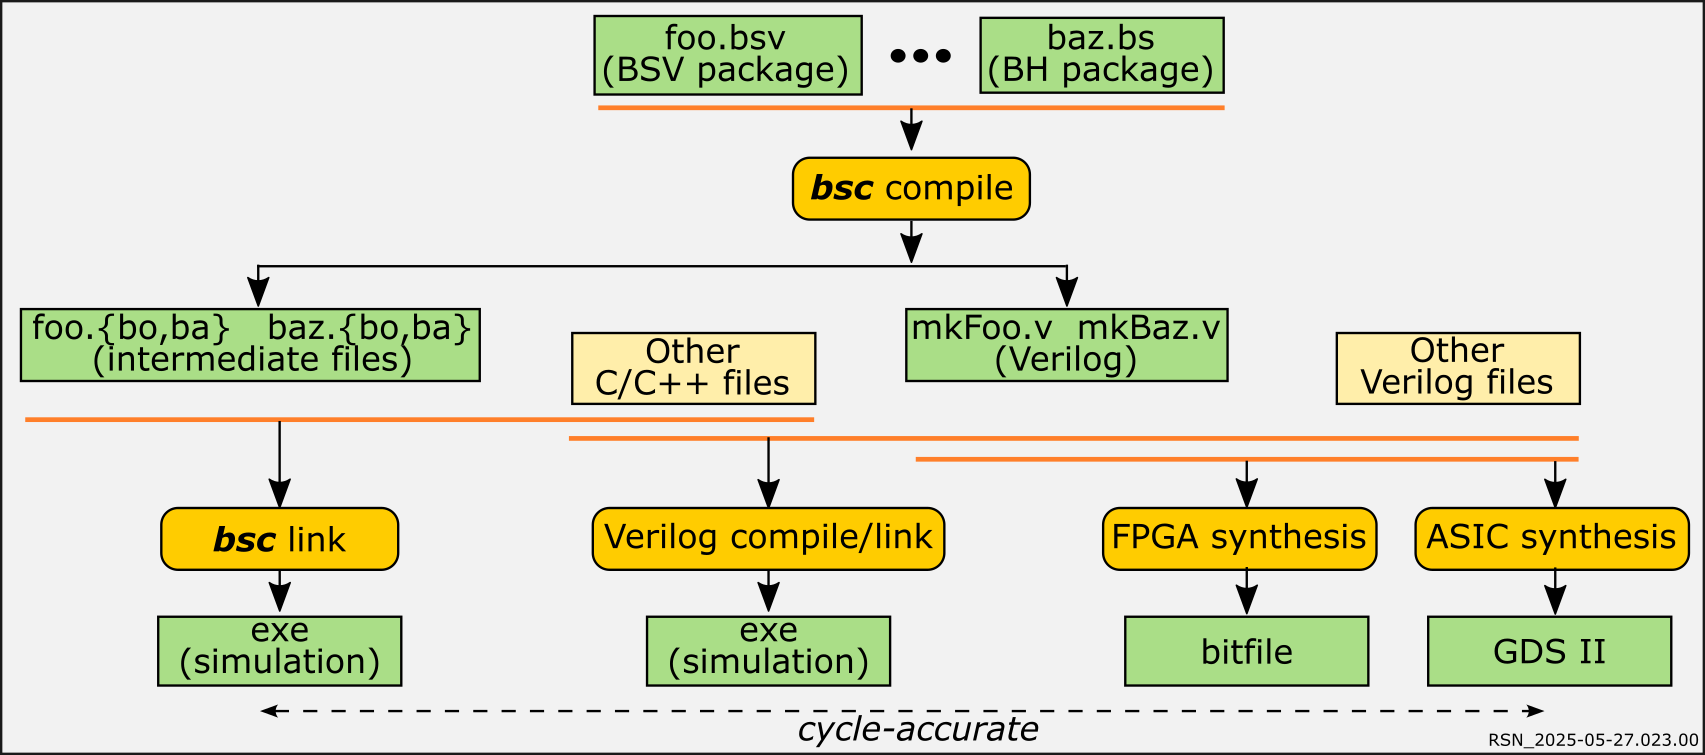
\includegraphics[width=\textwidth]
                  {Figures/RSN_2025-05-27.023.00_BLang_Build_Flows.png}
 \end{minipage}
 \hm
 \begin{minipage}{0.37\textwidth}\scriptsize

  \begin{itemize}

   \item For both FPGAs and ASICs, we proceed with the same Verilog
         that we have already generated for simulation, taking it
         through ``synthesis'' tools.

   \item Certain constructs in the Verilog are ignored by synthesis
         tools, notably {\tt \$display}, {\tt \$finish}, and imported
         C (and the synthesis tools will optimize away any logic that
         was only producing data for such statements).

   \item In both cases, we need to add additional circuitry (and
         possibly intervening IPs) that connect our design to the
         ``pins'' of the FPGA/ASIC, for data I/O.

   \item For FPGAs the output is a ``bitfile'' that is then loaded
         into the FPGA to configure the FPGA to emulate our design.

   \item For ASICs the output is a ``GDS II'' file that is sent to a
         fabrication facility/foundry for rendering into silicon.

  \end{itemize}

 \end{minipage}
\end{center}

\end{frame}

% ****************************************************************
% ****************************************************************
% ****************************************************************

\begin{frame}[fragile]

\frametitle{Thank you!}

\begin{center}
 \hm
 \begin{minipage}{0.5\textwidth}
  \tableofcontents

  \vspace*{10ex}

  \hmmmm {\bf Q \& A?}
 \end{minipage}
 \hmm
 \begin{minipage}{0.4\textwidth}\scriptsize\it
  \vstrut{0em}{20ex} \\
  \fbox{
   \begin{minipage}{\textwidth}\scriptsize\it
    {\bf Thank you!}
    \begin{tabbing} % Verse
      Dear friends, about CPU design \\
      \hmm We've just had a lightning preview, \\
      We've left you with all the materials \\
      \hmm As programmers you can see, its not anything new! \\
      We hope you're inspired to go try it later \\
      \hmm And take flight on your own! Whoo hoo! \\
      \\
      It's been a pleasure for me to share this, \\
      \hmm So from me, a sincere Thank You!
    \end{tabbing}
   \end{minipage}}
 \end{minipage}
\end{center}

\end{frame}

% ================================================================

\begin{frame}[fragile]
\frametitle{Links to additional resources (all free and open-source):}

\emph{bsc} compiler for BSV and BH, libraries, discussion forums:
{\scriptsize
\begin{tabbing}
\hmmm \= \href{https://github.com/B-Lang-org/bsc}{https://github.com/B-Lang-org/bsc} \\
      \> \href{https://groups.io/g/b-lang-discuss}{https://groups.io/g/b-lang-discuss} \\
      \> \href{https://groups.io/g/b-lang-announce/topics}{https://groups.io/g/b-lang-announce/topics} \\
      \> \href{https://github.com/B-Lang-org/bsc-contrib}
              {https://github.com/B-Lang-org/bsc-contrib} \hmm (incl. AMBA/AXI fabrics) \\
      \> \href{https://github.com/BSVLang/Main}
              {https://github.com/BSVLang/Main}
\end{tabbing}}

Textbook, lecture slides, exercises, full code for {\DRUM} and {\FIFE}
RISC-V CPUs (buildable, runnable):

{\scriptsize
\begin{tabbing}
\hmmm \href{https://github.com/rsnikhil/Learn_Bluespec_and_RISCV_Design}
           {https://github.com/rsnikhil/Learn\_Bluespec\_and\_RISCV\_Design}
\end{tabbing}}

RISC-V CPUs (all RV64GC, Linux-capable, coded in BSV):
{\scriptsize
\begin{tabbing}
\hmmm \= CHERI (RISC-V + security capabilities): \hm \= \kill
      \> Piccolo (3-stage)                   \> \href{https://github.com/bluespec/Piccolo}
                                                     {https://github.com/bluespec/Piccolo} \\
      \> Flute (5-stage)                     \> \href{https://github.com/bluespec/Flute}
                                                     {https://github.com/bluespec/Flute} \\
      \> Toooba (Superscalar, out-of-order)  \> \href{https://github.com/bluespec/Toooba}
                                                     {https://github.com/bluespec/Toooba} \\
      \> CHERI (RISC-V + security capabilities): \> \href{https://github.com/CTSRD-CHERI}
                                                     {https://github.com/CTSRD-CHERI}
                                                \hmm (U.Cambridge)
\end{tabbing}}

RISC-V IP (coded in BSV):
{\scriptsize
\begin{tabbing}
\hmmm \= CHERI (RISC-V + capabilities):  \hm \= \kill
      \> CLINT (timer and sw intertupts)     \> \href{https://github.com/bluespec/CLINT}
                                                     {https://github.com/bluespec/CLINT} \\
      \> PLIC (interrupt controller)         \> \href{https://github.com/bluespec/PLIC}
                                                     {https://github.com/bluespec/PLIC} \\
      \> Debug Module                        \> \href{https://github.com/bluespec/RISCV_Debug_Module}
                                                     {https://github.com/bluespec/RISCV\_Debug\_Module} \\
      \> gdbstub                             \> \href{https://github.com/bluespec/RISCV_gdbstub}
                                                     {https://github.com/bluespec/RISCV\_gdbstub}
\end{tabbing}}

\end{frame}

% ================================================================

% -*- mode: fundamental -*-

% Postamble that is shareable across slide decks

% Copyright (c) 2025 Rishiyur S. Nikhil, All Rights Reserved

% ================================================================

\begin{frame}

\begin{center}

\vspace*{15ex}

\begin{minipage}{0.5\textwidth}\scriptsize
  Slides preparation tools:
  \begin{itemize}
   \item Text and layout: LaTeX with Beamer package, Madrid theme
   \item Diagrams: Inkscape for SVG; Inkscapet to export to PNG
  \end{itemize}
\end{minipage}

\end{center}

\end{frame}

% ================================================================


% ================================================================

\end{document}
